% !TeX root = main.tex
\def\kurt{\mathop{\mathsf{kurt}}}
\def\MI{\mathop{\mathsf{MI}}}
\def\KL{\mathop{\mathsf{D}_{\mathsf{KL}}}}

\section{Independent Component Analysis}\autocite{hyvarinen2000,cover2006}

\textbf{Notation in this Chapter}\\
{\small
\begin{itemize}
  \item $\vect x$ is a random vector of $n$ sensor measurements (here $x_i$ is the $i$-th \emph{component}, not the $i$-th training sample).
  \item $\vect s=(s_1,\dots,s_m)^T$ are the (latent) source signals ($m$ sources; later we assume $m=n$).
  \item $\mat A$ mixing matrix, $\mat W$ unmixing matrix.
  \item Observed realizations: $\vect x(1),\dots,\vect x(T)$.
  \item $E\{\cdot\}$ denotes expectation (often approximated by the sample mean over $t=1,\dots,T$).
  \item $\vect{\tilde x}$: whitened (decorrelated) version of $\vect x$.
  \item $\hat{\vect s}$: estimated sources.
  \item $y=\vect w^T\vect x$: a projection (scalar), \emph{not} a class label.
\end{itemize}
}

\subsection{Motivation - Cocktail-Party Problem}
  The classical motivation for ICA is the cocktail-party problem. Imagine the following situation: two microphones are placed in a room at different locations, and they record the time signals $x_1(t), x_2(t)$. Two speakers $s_1(t), s_2(t)$ are talking at the same time, and each recorded signal is a weighted sum of the two speakers:
 \begin{eqnarray*}
      x_1(t) &=& a_{11} s_1(t) + a_{12} s_2(t) \\
      x_2(t) &=& a_{21} s_1(t) + a_{22} s_2(t)
    \end{eqnarray*}

    The parameters $a_{ij}$ depend on the distance of the microphones to the speakers. For simplicity, we assume just a very simple mixing model without any time delays, reflections, or other factors.  

   \textbf {Observations:} if we knew the $a_{ij}$, reconstructing the $s_i$ would only require solving a system of linear equations by classical methods. \textbf{But:} we do not know the $a_{ij}$! Thus, the problem is considerably more difficult. The goal is to estimate an unmixing from the recorded mixtures alone, without knowing the sources or the mixing process (blind source separation). In the lecture example, one source is a person speaking and the other a piano playing; both microphones record a superposition of the two with different relative loudness, and the separated outputs recover the speech and the piano.
  
  The principle for solving the cocktail-party problem has a lot of \textbf {other interesting applications}: speech signal recovery in telecommunications, recovery of images from mixed signals in MRI and fMRI, electrical recordings of brain activity such as EEG (electroencephalography) and MEG (magnetoencephalography), where ICA isolates and localizes independent sources of brain activity, feature extraction, and multispectral image analysis. ICA can, for example, also separate a mixture of natural images into its individual source images, although the recovered sources may appear in a different order (permuted) than the original ones.

 \textbf{Common framework.}
 The \textbf {idea} is to use some information about the statistical properties of the signals $s_i(t)$ to estimate the $a_{ij}$. Surprisingly, it turns out that the only statistical assumption that we have to make is that the $s_i(t)$ are \textit{statistically independent} at each time point $t$.
 The formulation of this idea in a unified mathematical framework (H\'{e}rault and Jutten, 1984-1991) is
  \begin{center}
   \textbf {ICA -- Independent Component Analysis}
  \end{center}

\subsection{Latent Variables and Factor Analysis}

Latent means hidden. 
 \textbf {Statistical latent variables model:}
  \begin{itemize}
    \item Rewrite the time series into $n$ linear mixture observations $x_1, \ldots, x_n$            
    \item Each mixture $x_i$ as well as each component $s_j$ are random variables
  \end{itemize}
  \begin{displaymath}
    x_i = \sum_{j=1}^m a_{ij} s_j ~, \qquad i = 1,\ldots,n
  \end{displaymath}

  In matrix notation:
  \begin{displaymath}
    \vect x = \mat A \vect s
  \end{displaymath}

  where
  \begin{itemize}
    \item $\mat A$ is a constant \textit{mixing} matrix
    \item $s_j$ are latent random variables (independent components)
    \item both $\mat A$ and $s_j$ have to be estimated based on observations $x_i$
  \end{itemize}
         
 \subsubsection {First Approach: Decorrelation}

  Assuming $E\{\vect x\} = \vect{0}$, we already know a latent variable representation \\
  (see the feature transform in Chapter \emph{Discriminant Analysis}).

  From:
  \begin{displaymath}
      E\{ \vect x \vect x^T \} = \mat \Sigma = \mat U \mat D \mat U^T
  \end{displaymath}
  and
  \begin{displaymath}
    \mat{\Sigma}^{-1} 
    = \mat{U}\mat{D}^{-1}\mat{U}^T
    = (\mat{U}\mat{D}^{-\frac{1}{2}})\cdot \mat{I} \cdot(\mat{U}\mat{D}^{-\frac{1}{2}})^T
  \end{displaymath}

  we compute, for zero-mean vectors, the mapping:
  \begin{displaymath}
    \vect{\tilde{x}} = \mat D^{-\frac{1}{2}} \mat U^T \vect x
  \end{displaymath}
  is called \textbf   {\textit{Whitening Transform}}. It has some interesting properties:
  \begin{itemize}
    \item The mapped random variables $\tilde{x}_i$ are uncorrelated.            
    \item $\vect{\tilde{x}}$ has unit variance:
  \end{itemize}

  \begin{eqnarray*}
     E\{ \vect{\tilde{x}} \vect{\tilde{x}}^T \} 
     &=& E\left\{ \Big( \mat D^{-\frac{1}{2}} \mat U^T \vect x \Big) \Big( \mat D^{-\frac{1}{2}} \mat U^T \vect x \Big)^T \right\}             
     = E\left\{ \mat D^{-\frac{1}{2}} \mat U^T \vect x \vect x^T \mat U \mat D^{-\frac{1}{2}} \right\} \\             
     &=& \mat D^{-\frac{1}{2}} \mat U^T \mat \Sigma \mat U \mat D^{-\frac{1}{2}} = \mat D^{-\frac{1}{2}} \mat U^T \cdot \mat U \mat D \mat U^T \cdot \mat U \mat D^{-\frac{1}{2}} \\             
     &=& \mat D^{-\frac{1}{2}} \mat D \mat D^{-\frac{1}{2}}             
     = \mat I
  \end{eqnarray*}
 
  We could interpret the mapped random variable $\vect{\tilde{x}}$ as an estimate of the latent variable model:
  \begin{displaymath}
    \hat{\vect s} = \vect{\tilde x}
  \end{displaymath}
  But this would give poor results.                      

 \textbf {Problem:} The whitening transform is not unique!              
  Consider for example an arbitrary orthogonal matrix $\mat R \in \real^{n \times n}$:
%
  \small
  \begin{eqnarray*}
    \vect x' 
    &=& \mat R \, \vect{\tilde x} = \mat R \, \mat D^{-\frac{1}{2}} \mat U^T \vect x \\[.2cm]
    E\{ \vect x' \, \vect x'^T \}
    &=& E\left\{ \mat R \left(\mat D^{-\frac{1}{2}} \mat U^T \vect x \right) \left( \mat D^{-\frac{1}{2}} \mat U^T \vect x \right)^T \mat R^T \right\} \\             
    &=& \mat R \mat I \mat R^T \\             
    &=& \mat I
  \end{eqnarray*}
         
\subsubsection{Second Approach: Independence}

 \textbf{Observations:}
  
  \begin{itemize}
    \item Lack of correlation determines the second-degree cross-moments (covariances) of a multi-variate distribution.
    \item Statistical independence is stronger, as it determines all of the cross-moments. 
  \end{itemize}

  Given 2 statistically independent random variables $y_1, y_2$ and 2 functions $h_1, h_2$:
  \footnotesize
  \begin{eqnarray*}
    E\{ h_1(y_1) \, h_2(y_2) \}
    &=& \iint h_1(y_1) \, h_2(y_2) \, p(y_1, y_2) \, \mathsf{d}y_1 \, \mathsf{d}y_2 \\             
    &=& \iint h_1(y_1) \, p(y_1) \, h_2(y_2) \, p(y_2) \, \mathsf{d}y_1 \, \mathsf{d}y_2 \\            
    &=& \int h_1(y_1) \, p(y_1) \, \mathsf{d}y_1 \int h_2(y_2) \, p(y_2) \, \mathsf{d}y_2 \\             
    &=& E\{ h_1(y_1) \} \, E\{ h_2(y_2) \}
  \end{eqnarray*}
   
  These extra moment conditions allow us to identify $\mat A$, but only up to a permutation and a non-zero scaling (including the sign) of its columns, and only if at most one source is Gaussian (see the ambiguities below). 

 \textbf {Case of Gaussian distribution:}
  
  \begin{itemize}
    \item Gaussian distribution is determined by its second moments alone.
    \item Any Gaussian independent components can be determined only \\
      up to a rotation
  \end{itemize}
  \vspace{0.5\baselineskip}

  Therefore, we assume that the $s_i$ are \textbf{independent} and \textbf{non-Gaussian}.

\subsubsection{Whitening Transform}

  The whitening transform is usually done before ICA as a pre-processing step:

  \begin{itemize}
    \item Mixing matrix $\mat A$ has $n^2$ degrees of freedom.
    \item Whitening transforms the mixing matrix $\mat A$ into $\mat{\widetilde A}$:
      \begin{displaymath}
        \widetilde{\vect x} = \mat D^{-\frac{1}{2}} \, \mat U^T \, \mat A \, \vect s = \mat{\widetilde A}\, \vect s
      \end{displaymath}
    \item The new mixing matrix is \textbf{orthogonal} (assuming unit-variance sources $E\{\vect s\vect s^T\}=\mat I$):
      \begin{displaymath}
        E\big\{ \widetilde{\vect x}\,\widetilde{\vect x}^T \big\} = \mat{\widetilde A}\, E\big\{\vect s\, \vect s^T\big\} \, \mat{\widetilde A}^T = \mat I
      \end{displaymath}
    \item $\mat{\widetilde A}$ is orthogonal and has \textbf{$n (n-1) / 2$ degrees of freedom}.
  \end{itemize}

  Thus, applying the whitening transform solves roughly half of the problem.

\subsection{Illustration of ICA}

  Consider two independent components with the following uniform distributions:

  \begin{displaymath}
    p(s_i) = \begin{cases}
      \frac{1}{2\sqrt{3}} \quad &, ~\mbox{if}~|s_i| \leq \sqrt{3} \\
      0 \quad &, ~\mbox{otherwise}
    \end{cases}
  \end{displaymath}

  \textbf{Properties of the joint pdf:}
  \begin{itemize}
    \item signal components are independent.
    \item joint pdf is uniform on a square.
    \item zero mean.
    \item variance is equal to one.
  \end{itemize}

  The two independent components are mixed with the matrix:
  \begin{displaymath}
    \mat A = \left(
      \begin{array}{cc}
        2 & 3 \\
        2 & 1
      \end{array}
    \right),
    \quad \mbox{which results in}~ \vect x = \mat A \, \vect s ~.
  \end{displaymath}

  \textbf{Properties of the mixed signal:}
  \begin{itemize}
    \item joint pdf of mixed signals is uniform on a parallelogram.
  \end{itemize}

  More important: $x_1, x_2$ are not independent any more.

  \textbf{Intuitive way of estimating $\mat A$:}
  \begin{itemize}
    \item Edges of the parallelogram are in the directions of the columns of $\mat A$.
    \item In principle, we could first estimate the joint pdf of $x_1, x_2$.
    \item If we locate the edges of the joint pdf, we can estimate $\mat A$.
  \end{itemize}

  \textbf{But:}
  \begin{itemize}
    \item Computationally quite expensive.
    \item This principle works only with \textbf{exactly uniform} distributions.
  \end{itemize}

  Effect of the whitening transform applied to the data (Fig.~\ref{fig:ica_whitening}).

  \begin{figure}[htbp]
    \centering
    \begin{tikzpicture}
      \begin{groupplot}[group style={group size=3 by 1, horizontal sep=1.25cm},
          width=4.35cm, height=4.35cm, axis equal image, tick label style={font=\scriptsize},
          label style={font=\small}, title style={font=\small}]
        \nextgroupplot[title={Sources $\vect s$}, xlabel={$s_1$}, ylabel={$s_2$}, xmin=-2.6, xmax=2.6, ymin=-2.6, ymax=2.6]
          \addplot[only marks, mark=*, mark size=0.5pt, blue!70] coordinates {(0.43,-0.59) (1.38,1.51) (0.96,-1.19) (-0.95,0.05) (-0.69,-1.41) (1.29,1.61) (-1.71,0.26) (1.11,1.05) (1.03,-0.76) (-0.11,1.05) (-0.68,0.70) (-0.77,0.50) (-0.85,1.56) (-0.19,-0.23) (0.02,-0.29) (0.19,0.67) (1.72,1.16) (1.01,-0.57) (0.42,0.59) (1.69,-1.01) (-0.99,0.18) (-1.18,0.93) (0.39,-1.51) (-1.58,0.79) (-1.61,-1.68) (0.05,1.59) (-0.12,-0.11) (1.45,-0.31) (0.45,0.76) (0.05,0.08) (-0.01,0.80) (-0.87,-1.44) (-1.69,0.22) (-1.07,0.20) (0.67,1.50) (-1.04,-1.59) (-0.45,-0.16) (-1.72,0.45) (1.14,0.18) (-1.20,-1.48) (-0.81,0.32) (1.32,-0.96) (0.03,-1.05) (1.20,1.31) (0.48,-1.05) (0.84,-0.16) (-1.42,0.87) (0.14,0.72) (0.03,0.19) (1.29,1.06) (-0.48,-0.12) (0.34,0.42) (-1.53,1.10) (-0.39,0.62) (-0.61,0.49) (-1.21,-0.33) (1.10,0.20) (-0.42,-0.36) (1.66,0.85) (0.31,-0.41) (0.36,-0.12) (0.48,0.88) (0.61,0.01) (-1.21,-0.56) (-0.21,1.13) (-0.90,-0.41) (-0.34,1.19) (-1.40,0.99) (1.62,-0.18) (-0.99,0.74) (0.60,-1.61) (-0.69,-0.38) (1.30,1.25) (0.56,0.28) (-1.28,0.20) (1.20,0.57) (1.54,0.62) (1.40,0.29) (0.24,-0.27) (-1.23,-1.10) (-1.07,-0.72) (1.48,-0.72) (0.18,-0.24) (-1.11,1.73) (1.33,-0.51) (0.49,-0.18) (0.24,-0.44) (-0.43,0.28) (-0.31,1.55) (-0.90,1.35) (-1.60,-0.43) (1.30,-0.81) (-0.11,1.33) (0.17,-0.02) (-0.62,0.64) (0.87,-1.48) (-1.64,1.27) (-0.44,-0.65) (-1.63,-0.02) (-1.31,-1.05) (1.62,-0.28) (0.55,1.14) (-0.25,1.13) (0.08,-0.09) (1.29,0.93) (-0.54,-0.15) (0.31,-0.44) (0.64,0.16) (-0.50,-1.03) (0.07,-0.64) (0.92,0.72) (1.42,0.94) (-1.21,-1.54) (1.50,0.81) (-1.71,1.10) (0.88,-0.19) (1.08,-1.52) (-1.26,0.63) (-0.28,-0.88) (1.09,0.50) (-1.68,-0.43) (0.45,0.48) (1.02,-0.84) (0.05,-0.08) (0.78,0.09) (-0.95,0.45) (-1.04,-1.03) (-0.47,1.60) (-1.11,-0.73) (-0.53,-0.67) (1.55,-0.84) (0.25,-1.50) (-0.55,-0.27) (-0.79,0.94) (1.57,0.73) (-0.19,-1.05) (1.66,-1.26) (0.05,-0.62) (0.07,0.93) (1.37,-0.04) (0.84,1.47) (0.28,0.54) (-0.25,0.42) (1.31,0.93) (-0.31,0.87) (1.46,-0.54) (-1.49,-0.84) (-0.24,-0.22) (0.07,-0.04) (1.56,-1.24) (-0.86,-0.20) (1.06,0.48) (0.61,-1.26) (0.75,-1.25) (0.45,-1.13) (1.63,-0.75) (-0.58,1.60) (-0.35,-1.64) (-1.03,-1.10) (-1.56,-1.16) (-0.99,-0.09) (1.44,-1.68) (1.18,-0.14) (-1.34,-1.17) (0.36,-0.80) (-0.07,1.01) (0.33,-1.09) (0.55,0.41) (-0.67,-0.32) (1.60,-0.29) (-0.12,1.10) (0.44,-1.17) (0.47,1.47) (-1.10,1.36) (-1.52,0.58) (-0.31,-1.56) (0.91,0.57) (1.09,0.35) (0.80,0.94) (-1.34,-0.99) (1.43,1.57) (1.05,1.34) (1.31,-1.34) (0.08,-0.64) (1.44,-1.62) (-1.57,1.15) (-1.63,1.44) (-1.66,1.70) (-0.86,0.39) (-0.87,0.57) (-1.08,0.62) (0.23,0.24) (-1.60,1.57) (0.31,0.37) (-1.16,-0.57) (0.62,0.04) (-1.66,-1.67) (-0.66,0.78) (1.52,0.67) (0.13,-0.27) (1.08,1.22) (0.55,0.89) (0.38,-0.57) (-1.07,-1.46) (0.26,-1.27) (-1.59,-1.09) (1.04,-0.68) (1.59,-0.18) (1.23,1.48) (-1.56,-0.77) (-0.56,1.38) (-0.63,0.63) (-1.34,1.22) (0.44,-0.34) (1.03,-1.72) (-0.65,0.99) (1.26,-0.88) (1.03,-1.24) (-1.28,1.04) (0.92,0.65) (1.33,-1.00) (-1.05,-0.81) (0.26,1.52) (0.48,-0.80) (0.38,0.70) (-1.40,-1.28) (0.56,1.09) (0.46,-1.32) (1.12,0.06) (1.05,-1.61) (-0.60,0.17) (0.77,1.20) (1.27,-1.44) (1.36,-0.78) (-1.17,0.92) (-1.64,0.37) (0.52,-0.65) (-0.99,0.45) (0.22,-0.16) (1.54,1.26) (-0.42,-0.72) (-0.86,0.89) (-0.15,0.47) (0.54,0.83) (-1.38,-0.42) (-0.41,0.78) (-1.27,0.69) (0.56,-0.39) (1.15,-1.64) (-0.43,1.60) (-0.44,0.74) (0.14,-1.02) (-0.99,0.80) (-0.87,-0.77) (-0.59,-0.11) (-0.15,1.25) (-1.45,-0.18) (0.88,-0.73) (0.27,-0.67) (-0.69,-1.47) (-1.46,-0.97) (0.91,-0.79) (-1.28,-1.13) (-1.27,-1.51) (-1.28,-0.12) (-1.45,-0.99) (1.41,0.83) (-0.80,1.46) (-0.67,-0.79) (1.15,0.25) (0.42,0.02) (-1.08,-1.47) (-0.23,-1.30) (1.33,1.33) (-0.43,-0.09) (0.73,1.06) (-1.40,-1.50) (0.79,0.33) (0.96,1.27) (1.13,1.27) (0.60,-1.71) (-0.45,0.08) (-1.51,-0.45) (0.07,0.90) (0.89,-1.48) (-1.07,-0.81) (-0.81,1.08) (0.13,-0.11) (0.86,-0.16) (1.37,1.62) (-1.30,-0.62) (-1.09,-1.59) (1.04,-0.37) (0.50,-1.20) (0.77,-1.45) (1.72,0.24) (1.52,1.57) (1.19,0.28) (0.96,0.51) (-0.36,-0.61) (0.49,0.25) (-1.09,0.87) (0.90,0.31) (0.89,1.05) (0.77,0.17) (-0.19,-1.05) (-0.42,0.29) (-0.28,-0.03) (-1.62,-1.16) (1.19,0.41) (0.15,1.10) (-0.39,-1.26) (0.17,0.16) (0.77,0.81) (-0.41,-0.34) (1.15,-0.80) (1.45,-0.44) (-0.39,0.14) (-1.25,0.65) (0.90,0.20) (1.71,-1.36) (-1.22,1.10) (0.74,1.47) (1.13,-1.38) (1.46,-0.87) (-1.30,-1.13) (-1.41,1.21) (1.69,1.42) (-1.33,-1.58) (-1.12,-0.58) (0.26,-1.07) (-0.19,-0.11) (0.87,1.46) (-1.07,-1.49) (1.44,-1.14) (-0.98,-0.04) (0.93,0.08) (-1.50,0.85) (-0.09,-0.22) (-1.62,-1.24) (-0.64,-0.51) (-0.65,1.67) (0.76,0.87) (-0.16,-1.33) (-1.54,1.07) (1.72,-0.65) (1.35,0.97) (1.44,-1.69) (-0.88,1.29) (-0.37,-1.17) (-0.95,-0.15) (-1.30,0.56) (-1.62,0.03) (0.01,-1.16) (-1.31,-1.25) (-1.12,-0.75) (1.25,-1.55) (-0.05,-0.98) (-1.10,-1.28) (0.59,-0.12) (-0.81,-0.50) (0.09,0.30) (-0.75,-0.76) (0.06,-1.61) (0.45,-0.59) (0.13,0.88) (-0.36,-0.85) (1.01,-0.33) (1.29,0.88) (-1.11,-0.32) (-1.26,1.34) (-1.34,1.45) (1.66,-0.66) (1.53,0.82) (-0.93,-0.86) (1.63,-1.25) (-1.01,-0.22) (0.02,0.35) (-0.01,1.51) (1.44,-1.23) (-1.59,0.74) (-0.64,-0.08) (0.35,-1.28) (-1.50,1.64) (-0.91,0.68) (-0.12,-1.29) (1.32,1.41) (0.90,-1.37) (1.14,-1.41) (0.90,-0.58) (0.72,1.52) (1.21,-1.62) (0.63,1.45) (0.82,0.39) (-0.69,-1.50) (-1.15,0.24) (0.89,-0.14) (-1.16,0.22) (1.45,0.82) (0.33,0.62)};
          \draw[thick] (axis cs:-1.732,-1.732) rectangle (axis cs:1.732,1.732);
        \nextgroupplot[title={Mixtures $\vect x=\mat A\vect s$}, xlabel={$x_1$}, ylabel={$x_2$}, xmin=-9.5, xmax=9.5, ymin=-9.5, ymax=9.5]
          \addplot[only marks, mark=*, mark size=0.5pt, red!70] coordinates {(-0.91,0.28) (7.29,4.26) (-1.67,0.72) (-1.75,-1.85) (-5.63,-2.80) (7.42,4.20) (-2.64,-3.17) (5.38,3.28) (-0.21,1.30) (2.91,0.82) (0.74,-0.66) (-0.04,-1.04) (2.98,-0.14) (-1.07,-0.61) (-0.85,-0.26) (2.37,1.04) (6.91,4.59) (0.31,1.46) (2.61,1.43) (0.36,2.38) (-1.44,-1.79) (0.44,-1.42) (-3.74,-0.73) (-0.79,-2.37) (-8.25,-4.90) (4.87,1.69) (-0.56,-0.34) (1.95,2.58) (3.19,1.66) (0.34,0.18) (2.38,0.78) (-6.06,-3.19) (-2.73,-3.16) (-1.53,-1.93) (5.82,2.83) (-6.86,-3.67) (-1.39,-1.07) (-2.08,-2.98) (2.81,2.46) (-6.82,-3.87) (-0.64,-1.29) (-0.25,1.67) (-3.10,-0.99) (6.34,3.72) (-2.17,-0.08) (1.20,1.52) (-0.23,-1.96) (2.44,1.00) (0.61,0.24) (5.76,3.64) (-1.32,-1.08) (1.93,1.10) (0.26,-1.95) (1.07,-0.16) (0.25,-0.73) (-3.40,-2.75) (2.80,2.39) (-1.92,-1.20) (5.86,4.16) (-0.62,0.21) (0.38,0.61) (3.61,1.84) (1.26,1.24) (-4.10,-2.98) (2.98,0.72) (-3.04,-2.22) (2.91,0.52) (0.17,-1.81) (2.69,3.06) (0.24,-1.24) (-3.65,-0.42) (-2.53,-1.76) (6.34,3.84) (1.95,1.40) (-1.95,-2.35) (4.10,2.96) (4.93,3.70) (3.67,3.09) (-0.34,0.21) (-5.75,-3.55) (-4.29,-2.85) (0.81,2.25) (-0.36,0.12) (2.97,-0.48) (1.13,2.15) (0.43,0.80) (-0.85,0.04) (-0.01,-0.58) (4.04,0.93) (2.24,-0.46) (-4.48,-3.63) (0.18,1.80) (3.77,1.11) (0.27,0.31) (0.70,-0.59) (-2.69,0.26) (0.52,-2.02) (-2.83,-1.53) (-3.31,-3.27) (-5.75,-3.66) (2.41,2.96) (4.50,2.23) (2.91,0.64) (-0.11,0.07) (5.37,3.51) (-1.52,-1.22) (-0.69,0.19) (1.75,1.43) (-4.11,-2.04) (-1.77,-0.50) (3.98,2.55) (5.65,3.77) (-7.02,-3.95) (5.42,3.81) (-0.13,-2.33) (1.18,1.56) (-2.40,0.64) (-0.62,-1.88) (-3.20,-1.44) (3.67,2.68) (-4.65,-3.79) (2.32,1.37) (-0.48,1.19) (-0.15,0.01) (1.82,1.65) (-0.53,-1.44) (-5.17,-3.12) (3.85,0.65) (-4.41,-2.95) (-3.08,-1.74) (0.57,2.26) (-3.99,-0.99) (-1.91,-1.38) (1.24,-0.64) (5.31,3.86) (-3.55,-1.44) (-0.44,2.07) (-1.75,-0.51) (2.93,1.08) (2.62,2.71) (6.08,3.15) (2.18,1.10) (0.75,-0.09) (5.40,3.55) (1.99,0.25) (1.31,2.39) (-5.51,-3.83) (-1.13,-0.70) (0.02,0.10) (-0.60,1.88) (-2.33,-1.93) (3.57,2.60) (-2.56,-0.04) (-2.26,0.25) (-2.49,-0.23) (1.02,2.52) (3.64,0.44) (-5.63,-2.35) (-5.34,-3.15) (-6.59,-4.27) (-2.26,-2.08) (-2.16,1.20) (1.92,2.21) (-6.19,-3.85) (-1.67,-0.08) (2.90,0.87) (-2.63,-0.44) (2.32,1.51) (-2.31,-1.66) (2.34,2.91) (3.06,0.86) (-2.64,-0.29) (5.34,2.40) (1.90,-0.83) (-1.29,-2.45) (-5.30,-2.17) (3.53,2.39) (3.23,2.53) (4.42,2.54) (-5.65,-3.67) (7.58,4.43) (6.11,3.43) (-1.39,1.28) (-1.76,-0.48) (-1.98,1.26) (0.30,-1.99) (1.06,-1.82) (1.77,-1.63) (-0.55,-1.33) (-0.02,-1.17) (-0.31,-1.55) (1.19,0.71) (1.51,-1.63) (1.75,1.00) (-4.02,-2.88) (1.37,1.28) (-8.32,-4.99) (1.02,-0.54) (5.05,3.71) (-0.55,-0.01) (5.81,3.38) (3.75,1.98) (-0.93,0.20) (-6.53,-3.60) (-3.31,-0.76) (-6.47,-4.28) (0.05,1.41) (2.64,3.01) (6.90,3.94) (-5.42,-3.88) (3.02,0.26) (0.61,-0.64) (0.99,-1.46) (-0.13,0.54) (-3.10,0.34) (1.69,-0.30) (-0.13,1.63) (-1.66,0.82) (0.54,-1.53) (3.79,2.49) (-0.34,1.65) (-4.51,-2.90) (5.07,2.03) (-1.44,0.16) (2.86,1.46) (-6.65,-4.08) (4.39,2.21) (-3.06,-0.41) (2.41,2.30) (-2.73,0.49) (-0.68,-1.02) (5.14,2.74) (-1.77,1.10) (0.38,1.94) (0.41,-1.43) (-2.16,-2.90) (-0.90,0.40) (-0.64,-1.53) (-0.03,0.28) (6.85,4.34) (-2.99,-1.55) (0.97,-0.82) (1.11,0.17) (3.59,1.92) (-4.03,-3.19) (1.51,-0.05) (-0.48,-1.85) (-0.04,0.74) (-2.63,0.65) (3.96,0.75) (1.33,-0.15) (-2.79,-0.75) (0.42,-1.17) (-4.05,-2.52) (-1.50,-1.29) (3.45,0.95) (-3.44,-3.08) (-0.45,1.02) (-1.47,-0.13) (-5.78,-2.85) (-5.84,-3.90) (-0.56,1.03) (-5.95,-3.69) (-7.08,-4.05) (-2.91,-2.68) (-5.87,-3.89) (5.30,3.64) (2.79,-0.14) (-3.70,-2.13) (3.06,2.56) (0.90,0.85) (-6.58,-3.64) (-4.35,-1.75) (6.66,3.99) (-1.13,-0.95) (4.63,2.52) (-7.30,-4.29) (2.56,1.90) (5.71,3.18) (6.07,3.53) (-3.93,-0.51) (-0.67,-0.82) (-4.38,-3.47) (2.83,1.03) (-2.65,0.31) (-4.58,-2.96) (1.63,-0.54) (-0.07,0.14) (1.23,1.56) (7.62,4.37) (-4.46,-3.22) (-6.95,-3.77) (0.95,1.70) (-2.60,-0.20) (-2.81,0.08) (4.15,3.68) (7.76,4.61) (3.20,2.65) (3.45,2.43) (-2.56,-1.34) (1.72,1.22) (0.44,-1.31) (2.73,2.11) (4.93,2.83) (2.06,1.71) (-3.52,-1.43) (0.02,-0.56) (-0.65,-0.59) (-6.70,-4.39) (3.62,2.80) (3.59,1.39) (-4.57,-2.04) (0.80,0.49) (3.96,2.35) (-1.83,-1.16) (-0.10,1.49) (1.58,2.46) (-0.35,-0.64) (-0.57,-1.86) (2.42,2.01) (-0.67,2.05) (0.86,-1.34) (5.88,2.94) (-1.89,0.87) (0.31,2.05) (-6.00,-3.74) (0.80,-1.62) (7.64,4.80) (-7.39,-4.23) (-3.98,-2.82) (-2.68,-0.55) (-0.69,-0.48) (6.12,3.20) (-6.61,-3.63) (-0.54,1.73) (-2.09,-2.00) (2.11,1.95) (-0.44,-2.15) (-0.83,-0.40) (-6.97,-4.48) (-2.81,-1.80) (3.71,0.37) (4.13,2.39) (-4.30,-1.64) (0.13,-2.00) (1.47,2.78) (5.62,3.67) (-2.18,1.20) (2.10,-0.47) (-4.24,-1.90) (-2.35,-2.04) (-0.92,-2.04) (-3.15,-3.21) (-3.45,-1.14) (-6.36,-3.86) (-4.48,-2.99) (-2.15,0.95) (-3.05,-1.09) (-6.04,-3.47) (0.81,1.05) (-3.11,-2.12) (1.09,0.49) (-3.78,-2.26) (-4.73,-1.50) (-0.86,0.31) (2.90,1.13) (-3.26,-1.57) (1.02,1.68) (5.24,3.47) (-3.19,-2.54) (1.50,-1.18) (1.66,-1.23) (1.35,2.67) (5.51,3.88) (-4.43,-2.72) (-0.49,2.01) (-2.67,-2.24) (1.11,0.40) (4.51,1.49) (-0.81,1.65) (-0.98,-2.45) (-1.53,-1.36) (-3.13,-0.58) (1.91,-1.37) (0.21,-1.15) (-4.10,-1.53) (6.86,4.04) (-2.32,0.43) (-1.95,0.87) (0.06,1.23) (5.99,2.96) (-2.43,0.81) (5.60,2.71) (2.79,2.02) (-5.87,-2.87) (-1.59,-2.07) (1.35,1.63) (-1.65,-2.09) (5.37,3.73) (2.53,1.29)};
          \draw[thick] (axis cs:8.660,5.196) -- (axis cs:-1.732,1.732) -- (axis cs:-8.660,-5.196) -- (axis cs:1.732,-1.732) -- cycle;
          \draw[-{Stealth}, very thick] (axis cs:0,0) -- (axis cs:3.464,3.464) node[above left, font=\scriptsize] {$\vect a_1$};
          \draw[-{Stealth}, very thick] (axis cs:0,0) -- (axis cs:5.196,1.732) node[below right, font=\scriptsize] {$\vect a_2$};
        \nextgroupplot[title={Whitened $\widetilde{\vect x}$}, xlabel={$\widetilde x_1$}, ylabel={$\widetilde x_2$}, xmin=-2.6, xmax=2.6, ymin=-2.6, ymax=2.6]
          \addplot[only marks, mark=*, mark size=0.5pt, green!50!black] coordinates {(-0.70,0.14) (0.12,-2.09) (-1.51,0.25) (0.75,0.59) (-0.48,1.53) (0.25,-2.12) (1.45,0.95) (-0.02,-1.57) (-1.25,-0.13) (0.86,-0.73) (1.02,-0.09) (0.94,0.13) (1.75,-0.63) (0.00,0.29) (-0.19,0.20) (0.37,-0.64) (-0.38,-2.06) (-1.11,-0.26) (0.14,-0.75) (-1.91,-0.39) (0.87,0.52) (1.54,0.07) (-1.32,0.87) (1.73,0.46) (-0.01,2.35) (1.12,-1.26) (0.04,0.15) (-1.23,-0.75) (0.25,-0.90) (0.05,-0.11) (0.61,-0.61) (-0.36,1.67) (1.40,0.97) (0.94,0.56) (0.62,-1.60) (-0.36,1.90) (0.24,0.42) (1.59,0.80) (-0.67,-0.92) (-0.16,1.92) (0.84,0.29) (-1.60,-0.17) (-0.74,0.77) (0.10,-1.82) (-1.06,0.46) (-0.68,-0.46) (1.67,0.28) (0.44,-0.66) (0.14,-0.17) (-0.14,-1.69) (0.29,0.40) (0.08,-0.56) (1.92,0.18) (0.75,-0.22) (0.82,0.03) (0.67,1.06) (-0.61,-0.91) (0.08,0.54) (-0.56,-1.78) (-0.49,0.09) (-0.31,-0.17) (0.32,-1.01) (-0.40,-0.44) (0.50,1.23) (0.99,-0.73) (0.39,0.91) (1.12,-0.69) (1.74,0.18) (-1.27,-0.97) (1.27,0.09) (-1.55,0.81) (0.26,0.75) (-0.01,-1.84) (-0.18,-0.60) (1.09,0.70) (-0.42,-1.26) (-0.64,-1.52) (-0.77,-1.18) (-0.34,0.03) (0.13,1.65) (0.29,1.26) (-1.55,-0.47) (-0.27,0.05) (2.06,-0.58) (-1.29,-0.52) (-0.45,-0.21) (-0.46,0.16) (0.54,0.06) (1.36,-0.99) (1.64,-0.43) (0.88,1.39) (-1.48,-0.28) (1.06,-0.95) (-0.10,-0.11) (0.93,-0.08) (-1.65,0.52) (2.12,0.13) (-0.11,0.78) (1.19,1.10) (0.23,1.67) (-1.33,-0.90) (0.45,-1.25) (1.02,-0.71) (-0.09,0.00) (-0.24,-1.59) (0.32,0.46) (-0.51,0.11) (-0.31,-0.56) (-0.34,1.11) (-0.47,0.43) (-0.12,-1.18) (-0.32,-1.68) (-0.19,1.97) (-0.48,-1.64) (2.05,0.31) (-0.74,-0.46) (-1.82,0.41) (1.39,0.36) (-0.39,0.85) (-0.40,-1.13) (0.94,1.45) (0.05,-0.68) (-1.30,-0.06) (-0.06,0.02) (-0.47,-0.61) (1.04,0.28) (0.05,1.48) (1.51,-0.91) (0.31,1.30) (-0.06,0.86) (-1.69,-0.42) (-1.22,0.96) (0.24,0.57) (1.27,-0.19) (-0.58,-1.62) (-0.58,0.92) (-2.06,-0.18) (-0.45,0.42) (0.64,-0.77) (-0.99,-0.91) (0.47,-1.70) (0.22,-0.61) (0.51,-0.16) (-0.25,-1.60) (0.87,-0.47) (-1.41,-0.59) (0.51,1.64) (0.05,0.32) (-0.04,-0.03) (-1.98,-0.12) (0.51,0.73) (-0.39,-1.10) (-1.31,0.54) (-1.40,0.43) (-1.10,0.54) (-1.68,-0.55) (1.59,-0.84) (-0.88,1.48) (-0.01,1.52) (0.33,1.92) (0.68,0.73) (-2.20,0.29) (-0.92,-0.70) (0.17,1.79) (-0.80,0.35) (0.80,-0.73) (-0.98,0.60) (-0.08,-0.69) (0.28,0.69) (-1.32,-0.88) (0.90,-0.77) (-1.12,0.58) (0.74,-1.45) (1.79,-0.31) (1.54,0.57) (-0.86,1.38) (-0.22,-1.06) (-0.51,-1.02) (0.13,-1.27) (0.29,1.65) (0.12,-2.18) (0.23,-1.74) (-1.86,0.12) (-0.48,0.42) (-2.16,0.25) (1.98,0.18) (2.23,-0.01) (2.44,-0.18) (0.92,0.27) (1.07,0.14) (1.25,0.25) (0.04,-0.35) (2.30,-0.13) (0.07,-0.51) (0.46,1.20) (-0.38,-0.46) (0.04,2.38) (1.06,-0.16) (-0.58,-1.55) (-0.26,0.11) (0.12,-1.67) (0.27,-1.06) (-0.65,0.16) (-0.24,1.83) (-1.06,0.78) (0.40,1.90) (-1.20,-0.20) (-1.25,-0.95) (0.20,-1.97) (0.60,1.63) (1.42,-0.69) (0.93,-0.06) (1.87,-0.04) (-0.52,-0.05) (-1.94,0.60) (1.20,-0.33) (-1.50,-0.19) (-1.59,0.23) (1.69,0.07) (-0.17,-1.13) (-1.63,-0.15) (0.21,1.31) (0.93,-1.34) (-0.89,0.27) (0.26,-0.80) (0.12,1.91) (0.41,-1.22) (-1.24,0.69) (-0.74,-0.81) (-1.87,0.50) (0.59,0.26) (0.33,-1.45) (-1.91,0.22) (-1.51,-0.34) (1.53,0.08) (1.48,0.81) (-0.81,0.13) (1.06,0.32) (-0.24,-0.04) (-0.18,-2.01) (-0.18,0.82) (1.28,-0.11) (0.47,-0.27) (0.23,-1.01) (0.73,1.24) (0.88,-0.33) (1.43,0.32) (-0.65,-0.10) (-1.96,0.46) (1.48,-0.94) (0.88,-0.28) (-0.80,0.67) (1.31,0.05) (0.12,1.16) (0.38,0.47) (1.02,-0.86) (0.95,1.11) (-1.12,-0.05) (-0.65,0.32) (-0.51,1.57) (0.39,1.72) (-1.19,-0.03) (0.14,1.71) (-0.13,2.00) (0.87,0.94) (0.37,1.72) (-0.39,-1.59) (1.65,-0.59) (-0.05,1.04) (-0.62,-0.98) (-0.25,-0.31) (-0.24,1.84) (-0.73,1.13) (0.02,-1.93) (0.28,0.35) (0.26,-1.31) (-0.03,2.08) (-0.30,-0.80) (0.24,-1.62) (0.12,-1.74) (-1.62,0.88) (0.41,0.23) (0.79,1.35) (0.63,-0.74) (-1.66,0.51) (0.22,1.33) (1.38,-0.29) (-0.13,-0.02) (-0.70,-0.47) (0.20,-2.18) (0.52,1.34) (-0.31,1.94) (-0.98,-0.43) (-1.18,0.56) (-1.55,0.57) (-1.04,-1.36) (0.05,-2.24) (-0.63,-1.03) (-0.30,-1.05) (-0.14,0.70) (-0.15,-0.53) (1.44,0.06) (-0.40,-0.86) (0.14,-1.41) (-0.40,-0.66) (-0.58,0.91) (0.54,0.06) (0.21,0.20) (0.37,1.96) (-0.53,-1.13) (0.71,-0.95) (-0.59,1.21) (0.02,-0.24) (0.05,-1.15) (0.09,0.52) (-1.36,-0.18) (-1.33,-0.66) (0.41,0.14) (1.39,0.34) (-0.47,-0.78) (-2.17,-0.13) (1.69,-0.03) (0.55,-1.63) (-1.76,0.28) (-1.64,-0.34) (0.17,1.73) (1.91,0.02) (-0.17,-2.24) (-0.14,2.09) (0.42,1.19) (-0.91,0.62) (0.09,0.19) (0.45,-1.71) (-0.26,1.85) (-1.81,-0.12) (0.70,0.68) (-0.58,-0.71) (1.71,0.35) (-0.06,0.21) (0.31,2.03) (0.13,0.81) (1.69,-0.84) (0.10,-1.19) (-0.80,1.11) (1.90,0.21) (-1.67,-0.67) (-0.24,-1.67) (-2.21,0.30) (1.58,-0.40) (-0.54,1.13) (0.60,0.74) (1.37,0.44) (1.21,1.06) (-0.80,0.86) (0.08,1.82) (0.31,1.31) (-1.97,0.32) (-0.63,0.77) (-0.09,1.70) (-0.48,-0.32) (0.26,0.91) (0.18,-0.30) (0.03,1.07) (-1.16,1.18) (-0.71,0.13) (0.57,-0.77) (-0.31,0.88) (-0.93,-0.44) (-0.27,-1.56) (0.60,0.99) (1.89,-0.18) (2.03,-0.21) (-1.63,-0.64) (-0.49,-1.67) (0.09,1.27) (-2.03,-0.16) (0.61,0.84) (0.27,-0.30) (1.11,-1.16) (-1.88,-0.05) (1.70,0.50) (0.43,0.49) (-1.13,0.73) (2.28,-0.24) (1.17,0.09) (-0.80,1.05) (0.08,-1.98) (-1.60,0.42) (-1.79,0.29) (-1.04,-0.18) (0.59,-1.65) (-1.99,0.40) (0.61,-1.54) (-0.28,-0.86) (-0.54,1.59) (1.03,0.59) (-0.71,-0.50) (1.02,0.60) (-0.43,-1.62) (0.23,-0.71)};
          \draw[thick] (-0.014,-2.491) -- (2.480,-0.147) -- (0.014,2.491) -- (-2.480,0.147) -- cycle;
      \end{groupplot}
    \end{tikzpicture}
    \caption{Illustration of ICA with the uniform sources and the mixing matrix $\mat A$ from above (400 samples). Left: the joint pdf of the sources is uniform on an axis-aligned square. Middle: after mixing, the data lie on a parallelogram whose edges point in the directions of the columns $\vect a_1=(2,2)^T$ and $\vect a_2=(3,1)^T$ of $\mat A$ (arrows scaled by $\sqrt3$); $x_1$ and $x_2$ are no longer independent. Right: after centering and whitening, $\widetilde{\vect x}=\mat D^{-\frac12}\mat U^T\vect x$, the data are again uniform on a square, but on a \emph{rotated} one. Only this rotation, i.\,e.\ the orthogonal matrix $\mat{\widetilde A}$, remains to be estimated.}
    \label{fig:ica_whitening}
  \end{figure}

  \textbf{Properties of the whitened observations:}
  \begin{itemize}
    \item Joint pdf of $\widetilde{\vect x}$ is uniform on a square, but on a \emph{rotated} square in general (not aligned with the coordinate axes).
    \item Components are determined except for rotation.
    \item Problem of recovering $\mat{\widetilde A}$ is much simpler.
  \end{itemize}

  \textbf{From the illustration to the estimation algorithm.}
  Figure~\ref{fig:ica_pipeline} summarizes the processing chain: after centering and whitening, only the rotation $\mat{\widetilde A}$ is unknown. Figure~\ref{fig:ica_kurtosis} shows how this rotation is found for the example above: projecting the whitened data onto all unit vectors $\vect w$ and measuring the non-Gaussianity of $\vect w^T\widetilde{\vect x}$ (here by the kurtosis, see Sec.~\ref{sec:ica_kurtosis}) gives maxima exactly in the source directions. Figure~\ref{fig:ica_deflation} shows how the weight vectors are found one after the other under the constraints of the algorithm in Sec.~\ref{sec:ica_algorithm}.

  \begin{figure}[htbp]
    \centering
    \begin{tikzpicture}[node distance=0.45cm and 0.45cm, font=\small,
        blk/.style={draw, rounded corners, minimum height=0.9cm, align=center, fill=gray!8},
        sig/.style={inner sep=1pt}, >={Stealth}]
      \node[sig] (s) {$\vect s$};
      \node[blk, right=of s] (A) {mixing\\$\mat A$ (unknown)};
      \node[sig, right=of A] (x) {$\vect x$};
      \node[blk, right=of x] (c) {centering\\$\vect x-E\{\vect x\}$};
      \node[blk, right=of c] (w) {whitening\\$\mat D^{-\frac12}\mat U^T$};
      \node[sig, right=of w] (xt) {$\widetilde{\vect x}$};
      \node[blk, fill=blue!8, below=0.9cm of xt, xshift=-3.0cm] (W) {unmixing $\mat W=(\vect w_1,\dots,\vect w_n)^T$\\maximize non-Gaussianity of $\vect w_i^T\widetilde{\vect x}$};
      \node[sig, left=0.8cm of W] (sh) {$\hat{\vect s}=\mat W\widetilde{\vect x}$};
      \draw[->] (s) -- (A); \draw[->] (A) -- (x); \draw[->] (x) -- (c); \draw[->] (c) -- (w); \draw[->] (w) -- (xt);
      \draw[->] (xt) |- (W); \draw[->] (W) -- (sh);
      \node[font=\scriptsize, gray!30!black, below=2pt of A.south west, anchor=north] {unobserved};
      \node[font=\scriptsize, above=1pt of w.north west, anchor=south west, xshift=-1.6cm] {pre-processing ($n(n-1)/2$ parameters left)};
    \end{tikzpicture}
    \caption{Processing chain of the basic ICA estimation algorithm (Sec.~\ref{sec:ica_algorithm}). The sources $\vect s$ and the mixing matrix $\mat A$ are unknown; only $\vect x$ is observed. Centering and whitening turn the unknown mixing into an orthogonal matrix $\mat{\widetilde A}$. The rows $\vect w_i^T$ of the unmixing matrix $\mat W$ are then found one after the other by maximizing the non-Gaussianity of the projections $\vect w_i^T\widetilde{\vect x}$. The estimate $\hat{\vect s}$ equals $\vect s$ up to scale, sign and order.}
    \label{fig:ica_pipeline}
  \end{figure}

  \begin{figure}[htbp]
    \centering
    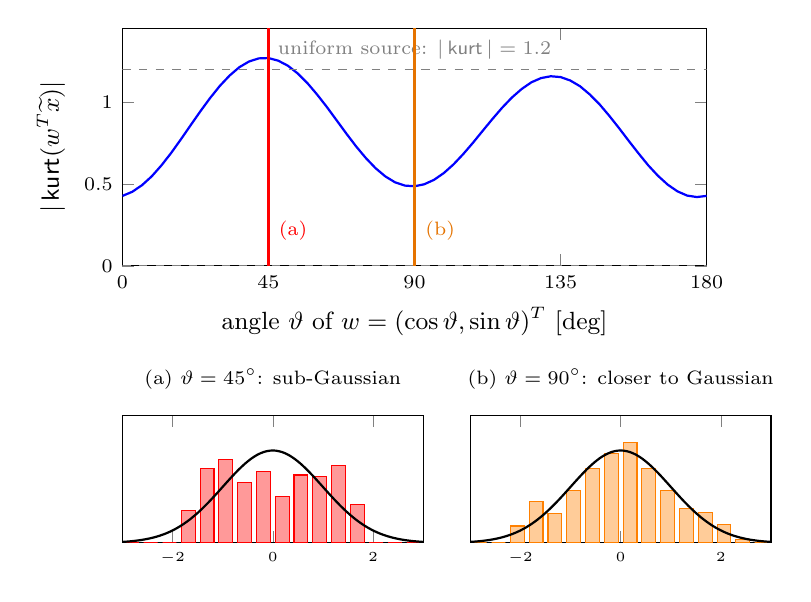
\begin{tikzpicture}
      \begin{axis}[name=kurt, width=9cm, height=4.6cm, xmin=0, xmax=180, ymin=0, ymax=1.45,
          xtick={0,45,90,135,180}, xlabel={angle $\vartheta$ of $\vect w=(\cos\vartheta,\sin\vartheta)^T$ [deg]},
          ylabel={$|\kurt(\vect w^T\widetilde{\vect x})|$}, tick label style={font=\scriptsize}, label style={font=\small}]
        \addplot[thick, blue] coordinates {(0,0.427) (3,0.452) (6,0.492) (9,0.546) (12,0.613) (15,0.689) (18,0.772) (21,0.858) (24,0.943) (27,1.024) (30,1.098) (33,1.161) (36,1.212) (39,1.247) (42,1.266) (45,1.268) (48,1.252) (51,1.221) (54,1.174) (57,1.115) (60,1.045) (63,0.969) (66,0.888) (69,0.807) (72,0.729) (75,0.658) (78,0.596) (81,0.546) (84,0.510) (87,0.490) (90,0.486) (93,0.498) (96,0.525) (99,0.566) (102,0.619) (105,0.682) (108,0.751) (111,0.824) (114,0.896) (117,0.965) (120,1.027) (123,1.079) (126,1.120) (129,1.146) (132,1.157) (135,1.152) (138,1.131) (141,1.096) (144,1.046) (147,0.986) (150,0.916) (153,0.841) (156,0.763) (159,0.687) (162,0.614) (165,0.550) (168,0.496) (171,0.455) (174,0.429) (177,0.420) (180,0.427)};
        \addplot[dashed, gray] coordinates {(0,1.2) (180,1.2)} node[pos=0.5, above, font=\scriptsize] {uniform source: $|\kurt|=1.2$};
        \addplot[dashed, gray] coordinates {(0,0) (180,0)};
        \addplot[red, thick] coordinates {(45,0) (45,1.45)} node[pos=0.15, right, font=\scriptsize] {(a)};
        \addplot[orange!90!black, very thick] coordinates {(90,0) (90,1.45)} node[pos=0.15, right, font=\scriptsize] {(b)};
      \end{axis}
      \begin{axis}[name=ha, at={(kurt.south west)}, anchor=north west, yshift=-1.9cm, width=5.4cm, height=3.2cm,
          xmin=-3, xmax=3, ymin=0, ymax=0.55, title={(a) $\vartheta=45^\circ$: sub-Gaussian}, title style={font=\scriptsize},
          tick label style={font=\tiny}, ytick=\empty]
        \addplot[ybar, bar width=5pt, fill=red!40, draw=red] coordinates {(-2.812,0.000) (-2.438,0.000) (-2.062,0.000) (-1.688,0.140) (-1.312,0.320) (-0.938,0.360) (-0.562,0.260) (-0.188,0.307) (0.188,0.200) (0.562,0.293) (0.938,0.287) (1.312,0.333) (1.688,0.167) (2.062,0.000) (2.438,0.000) (2.812,0.000)};
        \addplot[smooth, thick, black, domain=-3:3, samples=50] {exp(-x^2/2)/sqrt(2*pi)};
      \end{axis}
      \begin{axis}[at={(ha.east)}, anchor=west, xshift=0.6cm, width=5.4cm, height=3.2cm,
          xmin=-3, xmax=3, ymin=0, ymax=0.55, title={(b) $\vartheta=90^\circ$: closer to Gaussian}, title style={font=\scriptsize},
          tick label style={font=\tiny}, ytick=\empty]
        \addplot[ybar, bar width=5pt, fill=orange!40, draw=orange] coordinates {(-2.812,0.000) (-2.438,0.000) (-2.062,0.073) (-1.688,0.180) (-1.312,0.127) (-0.938,0.227) (-0.562,0.320) (-0.188,0.387) (0.188,0.433) (0.562,0.320) (0.938,0.227) (1.312,0.147) (1.688,0.133) (2.062,0.080) (2.438,0.013) (2.812,0.000)};
        \addplot[smooth, thick, black, domain=-3:3, samples=50] {exp(-x^2/2)/sqrt(2*pi)};
      \end{axis}
    \end{tikzpicture}
    \caption{Why maximizing non-Gaussianity finds the independent components (whitened data of Fig.~\ref{fig:ica_whitening}). Top: absolute kurtosis of the projection $\vect w^T\widetilde{\vect x}$ for all unit vectors $\vect w$. It is maximal (close to $1.2$, the value of a single uniform source) when $\vect w$ points along a source direction, and minimal halfway in between, where the projection is a sum of both sources and, by the central limit theorem, more Gaussian. Bottom: histograms of the projection (bars) against the standard normal pdf (black) at (a) a maximum and (b) a minimum of $|\kurt|$.}
    \label{fig:ica_kurtosis}
  \end{figure}

  \begin{figure}[htbp]
    \centering
    \begin{tikzpicture}[scale=1.25, >={Stealth}]
      \foreach \p in {(-0.70,0.14),(0.12,-2.09),(-1.51,0.25),(0.75,0.59),(-0.48,1.53),(0.25,-2.12),(1.45,0.95),(-0.02,-1.57),(-1.25,-0.13),(0.86,-0.73),(1.02,-0.09),(0.94,0.13),(1.75,-0.63),(0.00,0.29),(-0.19,0.20),(0.37,-0.64),(-0.38,-2.06),(-1.11,-0.26),(0.14,-0.75),(-1.91,-0.39),(0.87,0.52),(1.54,0.07),(-1.32,0.87),(1.73,0.46),(-0.01,2.35),(1.12,-1.26),(0.04,0.15),(-1.23,-0.75),(0.25,-0.90),(0.05,-0.11),(0.61,-0.61),(-0.36,1.67),(1.40,0.97),(0.94,0.56),(0.62,-1.60),(-0.36,1.90),(0.24,0.42),(1.59,0.80),(-0.67,-0.92),(-0.16,1.92),(0.84,0.29),(-1.60,-0.17),(-0.74,0.77),(0.10,-1.82),(-1.06,0.46),(-0.68,-0.46),(1.67,0.28),(0.44,-0.66),(0.14,-0.17),(-0.14,-1.69),(0.29,0.40),(0.08,-0.56),(1.92,0.18),(0.75,-0.22),(0.82,0.03),(0.67,1.06),(-0.61,-0.91),(0.08,0.54),(-0.56,-1.78),(-0.49,0.09),(-0.31,-0.17),(0.32,-1.01),(-0.40,-0.44),(0.50,1.23),(0.99,-0.73),(0.39,0.91),(1.12,-0.69),(1.74,0.18),(-1.27,-0.97),(1.27,0.09),(-1.55,0.81),(0.26,0.75),(-0.01,-1.84),(-0.18,-0.60),(1.09,0.70),(-0.42,-1.26),(-0.64,-1.52),(-0.77,-1.18),(-0.34,0.03),(0.13,1.65),(0.29,1.26),(-1.55,-0.47),(-0.27,0.05),(2.06,-0.58),(-1.29,-0.52),(-0.45,-0.21),(-0.46,0.16),(0.54,0.06),(1.36,-0.99),(1.64,-0.43),(0.88,1.39),(-1.48,-0.28),(1.06,-0.95),(-0.10,-0.11),(0.93,-0.08),(-1.65,0.52),(2.12,0.13),(-0.11,0.78),(1.19,1.10),(0.23,1.67),(-1.33,-0.90),(0.45,-1.25),(1.02,-0.71),(-0.09,0.00),(-0.24,-1.59),(0.32,0.46),(-0.51,0.11),(-0.31,-0.56),(-0.34,1.11),(-0.47,0.43),(-0.12,-1.18),(-0.32,-1.68),(-0.19,1.97),(-0.48,-1.64),(2.05,0.31),(-0.74,-0.46),(-1.82,0.41),(1.39,0.36),(-0.39,0.85),(-0.40,-1.13),(0.94,1.45),(0.05,-0.68),(-1.30,-0.06),(-0.06,0.02),(-0.47,-0.61),(1.04,0.28),(0.05,1.48),(1.51,-0.91),(0.31,1.30),(-0.06,0.86),(-1.69,-0.42),(-1.22,0.96),(0.24,0.57),(1.27,-0.19),(-0.58,-1.62),(-0.58,0.92),(-2.06,-0.18),(-0.45,0.42),(0.64,-0.77),(-0.99,-0.91),(0.47,-1.70),(0.22,-0.61),(0.51,-0.16),(-0.25,-1.60),(0.87,-0.47),(-1.41,-0.59),(0.51,1.64),(0.05,0.32),(-0.04,-0.03),(-1.98,-0.12),(0.51,0.73),(-0.39,-1.10),(-1.31,0.54),(-1.40,0.43),(-1.10,0.54),(-1.68,-0.55),(1.59,-0.84),(-0.88,1.48),(-0.01,1.52),(0.33,1.92),(0.68,0.73),(-2.20,0.29),(-0.92,-0.70),(0.17,1.79),(-0.80,0.35),(0.80,-0.73),(-0.98,0.60),(-0.08,-0.69),(0.28,0.69),(-1.32,-0.88),(0.90,-0.77),(-1.12,0.58),(0.74,-1.45),(1.79,-0.31),(1.54,0.57),(-0.86,1.38),(-0.22,-1.06),(-0.51,-1.02),(0.13,-1.27),(0.29,1.65),(0.12,-2.18),(0.23,-1.74),(-1.86,0.12),(-0.48,0.42),(-2.16,0.25),(1.98,0.18),(2.23,-0.01),(2.44,-0.18),(0.92,0.27),(1.07,0.14),(1.25,0.25),(0.04,-0.35),(2.30,-0.13),(0.07,-0.51),(0.46,1.20),(-0.38,-0.46),(0.04,2.38),(1.06,-0.16),(-0.58,-1.55),(-0.26,0.11),(0.12,-1.67),(0.27,-1.06),(-0.65,0.16),(-0.24,1.83),(-1.06,0.78),(0.40,1.90),(-1.20,-0.20),(-1.25,-0.95),(0.20,-1.97),(0.60,1.63),(1.42,-0.69),(0.93,-0.06),(1.87,-0.04),(-0.52,-0.05),(-1.94,0.60),(1.20,-0.33),(-1.50,-0.19),(-1.59,0.23),(1.69,0.07),(-0.17,-1.13),(-1.63,-0.15),(0.21,1.31),(0.93,-1.34),(-0.89,0.27),(0.26,-0.80),(0.12,1.91),(0.41,-1.22),(-1.24,0.69),(-0.74,-0.81),(-1.87,0.50),(0.59,0.26),(0.33,-1.45),(-1.91,0.22),(-1.51,-0.34),(1.53,0.08),(1.48,0.81),(-0.81,0.13),(1.06,0.32),(-0.24,-0.04),(-0.18,-2.01),(-0.18,0.82),(1.28,-0.11),(0.47,-0.27),(0.23,-1.01),(0.73,1.24),(0.88,-0.33),(1.43,0.32),(-0.65,-0.10),(-1.96,0.46),(1.48,-0.94),(0.88,-0.28),(-0.80,0.67),(1.31,0.05),(0.12,1.16),(0.38,0.47),(1.02,-0.86),(0.95,1.11),(-1.12,-0.05),(-0.65,0.32),(-0.51,1.57),(0.39,1.72),(-1.19,-0.03),(0.14,1.71),(-0.13,2.00),(0.87,0.94),(0.37,1.72),(-0.39,-1.59),(1.65,-0.59),(-0.05,1.04),(-0.62,-0.98),(-0.25,-0.31),(-0.24,1.84),(-0.73,1.13),(0.02,-1.93),(0.28,0.35),(0.26,-1.31),(-0.03,2.08),(-0.30,-0.80),(0.24,-1.62),(0.12,-1.74),(-1.62,0.88),(0.41,0.23),(0.79,1.35),(0.63,-0.74),(-1.66,0.51),(0.22,1.33),(1.38,-0.29),(-0.13,-0.02),(-0.70,-0.47),(0.20,-2.18),(0.52,1.34),(-0.31,1.94),(-0.98,-0.43),(-1.18,0.56),(-1.55,0.57),(-1.04,-1.36),(0.05,-2.24),(-0.63,-1.03),(-0.30,-1.05),(-0.14,0.70),(-0.15,-0.53),(1.44,0.06),(-0.40,-0.86),(0.14,-1.41),(-0.40,-0.66),(-0.58,0.91),(0.54,0.06),(0.21,0.20),(0.37,1.96),(-0.53,-1.13),(0.71,-0.95),(-0.59,1.21),(0.02,-0.24),(0.05,-1.15),(0.09,0.52),(-1.36,-0.18),(-1.33,-0.66),(0.41,0.14),(1.39,0.34),(-0.47,-0.78),(-2.17,-0.13),(1.69,-0.03),(0.55,-1.63),(-1.76,0.28),(-1.64,-0.34),(0.17,1.73),(1.91,0.02),(-0.17,-2.24),(-0.14,2.09),(0.42,1.19),(-0.91,0.62),(0.09,0.19),(0.45,-1.71),(-0.26,1.85),(-1.81,-0.12),(0.70,0.68),(-0.58,-0.71),(1.71,0.35),(-0.06,0.21),(0.31,2.03),(0.13,0.81),(1.69,-0.84),(0.10,-1.19),(-0.80,1.11),(1.90,0.21),(-1.67,-0.67),(-0.24,-1.67),(-2.21,0.30),(1.58,-0.40),(-0.54,1.13),(0.60,0.74),(1.37,0.44),(1.21,1.06),(-0.80,0.86),(0.08,1.82),(0.31,1.31),(-1.97,0.32),(-0.63,0.77),(-0.09,1.70),(-0.48,-0.32),(0.26,0.91),(0.18,-0.30),(0.03,1.07),(-1.16,1.18),(-0.71,0.13),(0.57,-0.77),(-0.31,0.88),(-0.93,-0.44),(-0.27,-1.56),(0.60,0.99),(1.89,-0.18),(2.03,-0.21),(-1.63,-0.64),(-0.49,-1.67),(0.09,1.27),(-2.03,-0.16),(0.61,0.84),(0.27,-0.30),(1.11,-1.16),(-1.88,-0.05),(1.70,0.50),(0.43,0.49),(-1.13,0.73),(2.28,-0.24),(1.17,0.09),(-0.80,1.05),(0.08,-1.98),(-1.60,0.42),(-1.79,0.29),(-1.04,-0.18),(0.59,-1.65),(-1.99,0.40),(0.61,-1.54),(-0.28,-0.86),(-0.54,1.59),(1.03,0.59),(-0.71,-0.50),(1.02,0.60),(-0.43,-1.62),(0.23,-0.71)} {\fill[green!50!black, opacity=0.4] \p circle (0.6pt);}
      \draw[thick, green!40!black] (-0.014,-2.491) -- (2.480,-0.147) -- (0.014,2.491) -- (-2.480,0.147) -- cycle;
      \draw[->, gray] (-2.6,0) -- (2.6,0) node[right] {$\widetilde x_1$};
      \draw[->, gray] (0,-2.6) -- (0,2.6) node[above] {$\widetilde x_2$};
      \draw[dashed] (0,0) circle (1);
      \node[font=\scriptsize, fill=white, inner sep=1pt] at (-0.55,-1.12) {unit circle};
      \draw[->, very thick, red] (0,0) -- (0.729,0.685) node[above right, black] {$\vect w_1$};
      \draw[->, very thick, blue] (0,0) -- (-0.683,0.731) node[above left, black] {$\vect w_2$};
      \draw (0.131,0.123) -- (0.008,0.255) -- (-0.123,0.131);
      \node[font=\scriptsize, align=left, anchor=west] at (1.25,-1.9) {$\|\vect w_i\|=1$,\\$\vect w_2^T\vect w_1=0$};
    \end{tikzpicture}
    \caption{The estimation algorithm of Sec.~\ref{sec:ica_algorithm} in the whitened space ($n=2$). In each iteration, $\vect w_i$ is searched on the unit circle (dashed), i.\,e.\ subject to $\|\vect w_i\|=1$. The first vector $\vect w_1$ converges to a direction of maximal non-Gaussianity, which is aligned with an edge of the rotated square and thus with one source. The second vector $\vect w_2$ must be orthogonal to $\vect w_1$; in two dimensions this leaves only one direction (up to sign), which is the remaining source direction. Stacking $\vect w_1^T,\vect w_2^T$ as rows gives $\mat W$.}
    \label{fig:ica_deflation}
  \end{figure}
  
 
\subsection{Properties of ICA}
 \textbf {Assumptions for the ICA model:}
  \begin{itemize}
    \item We assume that the $s_j$ are mutually independent.            
    \item The $s_j$ have to be non-Gaussian in order to determine them from the $x_i$.
    \item For simplicity, we assume that $\mat A$ is square, i.\,e.\ from now on $m=n$.
  \end{itemize}
 \textbf {Ambiguities of the ICA model:}
  \begin{itemize} 
    \item The $s_j$ are defined only up to a multiplicative constant.
    \item The $s_j$ are not ordered.
  \end{itemize}
 Writing the ICA model in terms of the columns of $\mat A$:
  \begin{displaymath}
    \vect x = \sum_{i=1}^n \vect a_i s_i            
  \end{displaymath}
  
  \begin{itemize}
    \item Any \textbf        {scalar multiplier} for $s_i$ can be eliminated by scaling $\vect a_i$ appropriately.            
    \item The matrix $\mat A$ can be adapted to restrict the $s_i$ to have \textbf        {unit variance}.            
    \item This still leaves the ambiguity of the \textbf        {sign}: \\
      multiplying $s_i$ by $\pm 1$ does not affect the model.            
    \item This ambiguity is usually \textbf        {insignificant} in most applications.
  \end{itemize}
 
 \textbf        {Ambiguity of the ordering:}
  \begin{displaymath}
    \vect x = \sum_{i=1}^n \vect a_i s_i
  \end{displaymath}
  \begin{itemize}
    \item As both $\vect s$ and $\mat A$ are unknown we can change the order of the summation.            
    \item Formalization using a \textbf        {permutation matrix $\mat P$}:
      \begin{displaymath}
        \vect x = \underbrace{\mat A \mat P}_{\mat A^{\ast}} \underbrace{\mat P^{-1} \vect s}_{\vect s^{\ast}}            
      \end{displaymath}
    \item $\mat A^{\ast}$ is just a new mixing matrix to be solved.
  \end{itemize}
 
\subsection{Basic Principle of ICA}

  So far, if we know $\mat A$, we could compute its inverse $\mat A^{-1}$ to obtain the independent components. Consider a linear combination of $x_i$ with a weight vector $\vect w$:
  \begin{displaymath}
    y = \vect w^T \vect x
  \end{displaymath}
  \vspace{0.5\baselineskip}

  Clearly, $y$ equals one of the independent components if $\vect w$ is one row of $\mat A^{-1}$.Change in variables:

  \begin{displaymath}
    \vect z = \mat A^T \vect w
  \end{displaymath}
  
  Applied to the linear combination:
 \begin{displaymath}
    y = \vect w^T \vect x = \vect w^T \mat A \vect s = \vect z^T \vect s
  \end{displaymath}
 
 \textbf{Result from the Central Limit Theorem:}

  \begin{itemize}
    \item The sum of a number of independent random variables tends toward a normal distribution.
    \item $\vect z^T \vect s$ is \textit{typically} more Gaussian than any of the $s_i$.
    \item $\vect z^T \vect s$ is \textit{least Gaussian} when it equals one of the $s_i$.
  \end{itemize}
 
 \textbf {Key principle of ICA:}         

  Maximizing the non-Gaussianity of $\vect w^T \vect x$ results in the independent components!\\[0.3cm]

 \textbf {Reasons for the importance of the non-Gaussianity:}             
 \begin{itemize}
    \item In case of Gaussian random variables, the ICA model can only be estimated up to an orthogonal transformation.                 
     \textbf{Note:}\\
      \quad If just one of the components is Gaussian, ICA still works.                             
    \item The Gaussian is the \textit{most random} distribution within the family of pdfs with given mean and variance.             
    \item Therefore, it is the least informative pdf with respect to the underlying data.
  \end{itemize}
  
  Distributions that have the \textit{least resemblance} to the Gaussian reveal more structure associated with the data.
 
\subsubsection{Importance of Non-Gaussianity}
  The \textit{randomness} can be measured using the concept of entropy from Shannon's information theory:
  \begin{itemize}
    \item Entropy is a measure of the uncertainty of an event, or the randomness of a measure.
  \end{itemize}
  \vspace{0.5\baselineskip}

\subsubsection{Differential Entropy}
  
  The \textit{differential entropy} of a continuous random variable $X$ with density $p(x)$ is defined as
    \begin{displaymath}
      H(x) = - \int p(x) \log p(x) \,\mathsf{d}x
    \end{displaymath}
  
\textbf{Theorem:}\\
    The Gaussian maximizes the entropy over all distributions with the same mean and the same covariance.\\
 \textbf {Proof:}   \\         

  \begin{itemize}
    \item Let $x$ be the random variable, $p(x)$ the pdf that has the highest randomness. \item Rewrite moments $M_i$ equations using a set of polynomials $\{ r_i(x) \}$:
      \begin{displaymath}
        \int p(x) r_i(x) \,\mathsf{d}x = M_i ~,~\mbox{where}~M_i~\mbox{are called moments}. \end{displaymath} 
    \item Using $r_0(x) \equiv 1$, $M_0 = 1$ constrains $p(x)$ to be a pdf.
  \end{itemize}
 
 \textbf{Lagrangian functional for the maximum entropy problem:}

  {\small
  \begin{displaymath}
    \argmin_{p(x)} \mathcal L(p) \equiv 
    \argmin_{p(x)} \int p(x) \log p(x) \,\mathsf{d}x - \sum_{i = 0}^N \lambda_i \left( \int p(x) r_i(x) \,\mathsf{d}x - M_i \right)
  \end{displaymath}
  }
  Taking the functional derivative with respect to $p(x)$ (G\^{a}teaux derivative) and setting it to zero:
%
  {\small
  \begin{displaymath}
    \frac{\delta \mathcal L}{\delta p} = \log p(x) + 1 - \sum_{i=0}^N \lambda_i r_i(x) \stackrel{!}{=} 0
  \end{displaymath}
  }
              
%  
  yields the family of exponential distributions:
%
  {\small
  \begin{displaymath}
    p(x) = \exp \left( -1 + \sum_{i=0}^N \lambda_i r_i(x) \right)
  \end{displaymath}
  } 
  Result for using first and second moments for mean $\mu$ and variance $\sigma^2$:
  \begin{displaymath}
    p(x) = e^{-(1 - \lambda_0 - \lambda_1 x - \lambda_2 (x-\mu)^2)}
  \end{displaymath}
  Plug the form into the constraints:
  \begin{eqnarray*}
    \int e^{-(1 - \lambda_0 - \lambda_1 x - \lambda_2 (x-\mu)^2)} \,\mathsf{d}x &=& 1 \\
    \int x e^{-(1 - \lambda_0 - \lambda_1 x - \lambda_2 (x-\mu)^2)} \,\mathsf{d}x &=& \mu \\
    \int (x-\mu)^2 e^{-(1 - \lambda_0 - \lambda_1 x - \lambda_2 (x-\mu)^2)} \,\mathsf{d}x &=& \sigma^2
  \end{eqnarray*}
 
  Integrate analytically (non-trivial) and solve for Lagrangian multipliers:
  \begin{eqnarray*}
    \lambda_0 &=& 1 - \frac{1}{2} \log(2 \pi \sigma^2 ) \\
    \lambda_1 &=& 0 \\
    \lambda_2 &=& - \frac{1}{2 \sigma^2}  
  \end{eqnarray*}
   
  Insert the results into the form of $p(x)$:
  \begin{eqnarray*}
    p(x) &=& e^{-(1 - \lambda_0 - \lambda_1 x - \lambda_2 (x-\mu)^2)} \\
         &=& e^{-\frac{1}{2} \log(2 \pi \sigma^2)} e^{-\frac{(x-\mu)^2}{2 \sigma^2}} \\
         &=& \frac{1}{\sqrt{2 \pi} \sigma} e^{- \frac{(x-\mu)^2}{2 \sigma^2}}
  \end{eqnarray*}
  
\subsection{ICA Estimation Algorithm}\label{sec:ica_algorithm}

 \textbf{Basic ICA Estimation Algorithm:}

  \begin{centernss}
    \begin{struktogramm}(105,50)
      \assign{Apply centering transform}
      \assign{Apply whitening transform}
      \assign{$i \gets 1$}
      \until{$i > n$~ ($n$: number of independent components)}
        \assign{Take a random vector $\vect w_i$}
        \assign{Maximize non-Gaussianity of $\vect w_i^T \vect{\tilde x}$ subject to $\| \vect w_i \| = 1$ and $\vect w_j^T \vect w_i = 0$, $j<i$}
        \assign{$i \gets i+1$}
      \untilend
      \assign{Use weight matrix $\mat W = \left( \vect w_1, \vect w_2, \ldots, \vect w_n \right)^T$ to compute $\hat{\vect s}=\mat W\vect{\tilde x}$}
      \assign{Output: independent components $\hat{\vect s}$ (up to scale, sign and order)}
    \end{struktogramm}
  \end{centernss}
  \vspace{0.3cm}
  
 \textbf {Notes:}\\

  \begin{itemize}
    \item Estimation by maximizing non-Gaussianity of independent components.            
    \item There exist equivalent algorithms for solving the ICA:
      \begin{itemize}
        \item Gradient descent methods
        \item Fast ICA
      \end{itemize}
                 
    \item Relation to Projection Pursuit approach (Friedman and Tukey, 1974):
      \begin{itemize}
        \item Projection Pursuit is a method for visualization and exploratory data analysis.
        \item Attempts to show clustering structure by finding \textit{interesting} projections.
        \item Interestingness is usually measured by non-Gaussianity.
      \end{itemize}
  \end{itemize}
 
\subsection{Measures of Non-Gaussianity}

these measures of gaussianity will be seen in other lectures, so it is good to understand them.  

  \begin{itemize}
    \item So far, we have seen that the key principle in estimating independent components is the non-Gaussianity.            
    \item In order to optimize the independent components, we need a quantitative measure of non-Gaussianity.
  \end{itemize}
 
  Consider the random variable $y$ and assume that it has zero mean and unit variance (enforced by pre-processing).  We will consider three measures of non-Gaussianity:

  \begin{itemize}
    \item\textbf        {Kurtosis}
    \item\textbf        {Negentropy}
    \item\textbf        {Mutual Information}
  \end{itemize}
          
\subsubsection{Kurtosis}\label{sec:ica_kurtosis}

\textbf{Definition}
 
   The \textbf {\textit{Kurtosis}} of $y$ is defined as:
    \begin{displaymath}
      \kurt(y) = E \{ y^4 \} - 3 \left( E\{ y^2 \} \right)^2
    \end{displaymath}
%    
    Since $y$ has unit variance, the equation simplifies to:
    \begin{displaymath}
      \kurt(y) = E \{ y^4 \} - 3
    \end{displaymath}    
    Additivity (for independent random variables $y_1, y_2$) and homogeneity:
    \begin{eqnarray*}
      \kurt(y_1 + y_2) &=& \kurt(y_1) + \kurt(y_2) \\
      \kurt(\alpha y) &=& \alpha^4 \kurt(y) ~, \quad \alpha \in \real
    \end{eqnarray*}
Kurtosis for a Gaussian distribution:
  
  \begin{itemize}
    \item The $n$-th central moment of a Gaussian distribution $p(y) = {\mathcal{N}}(y ; \mu, \sigma^2)$ with mean $\mu$ and variance $\sigma^2$ is:
      \begin{eqnarray*}
        E \{ (y - \mu)^n \} = \begin{cases}
                                (n-1) !! \cdot \sigma^n \quad &, ~n~ \mbox{even} \\
                                0 \quad &, ~n~ \mbox{odd}
                              \end{cases}
      \end{eqnarray*}
     \textbf{Note:}
      $(n-1)!!$ denotes the double factorial; for even $n$ we have $(n-1)!! = 1\cdot 3\cdot \dots \cdot (n-1)$.
    \item Thus, for a zero mean, unit variance random variable $y$ that is normally distributed:
      \begin{displaymath}
        \kurt(y) = 0
      \end{displaymath}
  \end{itemize}
 \textbf {Properties of Kurtosis:}

Figure~\ref{fig:kurtosis_densities} compares a sub-Gaussian, the Gaussian, and a super-Gaussian density.

  \begin{figure}[htbp]
    \centering
    \begin{tikzpicture}
      \begin{groupplot}[group style={group size=2 by 1, horizontal sep=1.3cm}, width=6.3cm, height=5cm,
          xmin=-4, xmax=4, xlabel={$y$}, tick label style={font=\scriptsize}, label style={font=\small}, title style={font=\small},
          legend style={font=\scriptsize, draw=none, fill=white, fill opacity=0.8, text opacity=1}, legend cell align=left]
        \nextgroupplot[title={densities $p(y)$}, ymin=0, ymax=0.75, legend to name=kurtleg, legend columns=3]
          \addplot[red, very thick, const plot] coordinates {(-4,0) (-1.7321,0.2887) (1.7321,0) (4,0)};
          \addlegendentry{uniform: $\kurt=-1.2$}
          \addplot[black, very thick, domain=-4:4, samples=121] {exp(-x^2/2)/sqrt(2*pi)};
          \addlegendentry{Gaussian: $\kurt=0$}
          \addplot[blue, very thick, domain=-4:4, samples=161] {exp(-sqrt(2)*abs(x))/sqrt(2)};
          \addlegendentry{Laplace: $\kurt=3$}
        \nextgroupplot[title={log scale: tails}, ymode=log, ymin=1e-4, ymax=1.5, ylabel={}]
          \addplot[red, very thick, const plot] coordinates {(-1.7321,0.2887) (1.7321,0.2887)};
          \draw[red, very thick] (axis cs:-1.7321,1e-4) -- (axis cs:-1.7321,0.2887) (axis cs:1.7321,1e-4) -- (axis cs:1.7321,0.2887);
          \addplot[black, very thick, domain=-4:4, samples=121] {exp(-x^2/2)/sqrt(2*pi)};
          \addplot[blue, very thick, domain=-4:4, samples=161] {exp(-sqrt(2)*abs(x))/sqrt(2)};
      \end{groupplot}
    \end{tikzpicture}

    \ref*{kurtleg}
    \caption{Three zero-mean, unit-variance densities with different kurtosis. The \emph{sub-Gaussian} uniform density ($\kurt=-1.2$) is flat and has no tails. The \emph{super-Gaussian} Laplace density $p(y)=\frac{1}{\sqrt2}e^{-\sqrt2|y|}$ ($\kurt=3$) has a sharp peak at zero and heavy tails: on the log scale (right) its tails decay only linearly, while the Gaussian ones decay quadratically. Since $\kurt$ measures the fourth moment relative to a Gaussian of the same variance, $|\kurt(y)|$ (or $\kurt(y)^2$) can serve as a measure of non-Gaussianity.}
    \label{fig:kurtosis_densities}
  \end{figure}

  \begin{itemize}
    \item Kurtosis is zero for a Gaussian random variable.            
    \item For most (but not all) non-Gaussian random variables, Kurtosis is nonzero.           \item Kurtosis can be positive or negative.            
    \item Typically, non-Gaussianity is measured as:
      \begin{itemize}
        \item\textbf        {$| \kurt(y) |$} ~ or
        \item\textbf        {$\kurt(y)^2$}
      \end{itemize}
  \end{itemize}
   
\textbf{Example}
        \textbf{\small \hspace{.5cm} Subgaussian pdf} (uniform, zero mean, unit variance), $\kurt(y)<0$:
        \begin{displaymath}
          p(y) = \begin{cases}
                   \frac{1}{2\sqrt{3}} \quad &, ~\mbox{if}~|y| \leq \sqrt{3} \\
                   0 \quad &, ~\mbox{otherwise}
                 \end{cases}
        \end{displaymath}
      
       \textbf  {\small \hspace{.5cm} Supergaussian pdf} (Laplace, zero mean, unit variance), $\kurt(y)>0$:
        {\footnotesize
        \begin{displaymath}
          p(y) = \frac{1}{\sqrt{2}} \exp(-\sqrt{2} |y|)
        \end{displaymath}
        }
   
  \begin{itemize}
    \item Consider 2-D case using the linear combination:
      \begin{eqnarray*}
        y        &=& \vect w^T \vect x = \vect w^T \mat A \vect s = \vect z^T \vect s = z_1 s_1 + z_2 s_2 \\
        \kurt(y) &=& \kurt(z_1 s_1) + \kurt(z_2 s_2) = z_1^4 \kurt(s_1) + z_2^4 \kurt(s_2)            
      \end{eqnarray*}
    \item As $y$ has unit variance, concerning also $s_1, s_2$:
      \begin{displaymath}
        E\{ y^2 \} = z_1^2 + z_2^2 = 1
      \end{displaymath}
      which constrains $\vect z$ to the unit circle in the 2-D plane.                     
    \item Thus, we have to find the maximum of the following function on the unit circle w.\,r.\,t.\ $\vect z$:
      \begin{displaymath}
        | \kurt(y) | = | z_1^4 \kurt(s_1) + z_2^4 \kurt(s_2) |
      \end{displaymath}
  \end{itemize}
 
 \textbf {Optimization landscape for Kurtosis in 2-D plane:}

  \begin{itemize}
    \item Thick curve is the unit circle
    \item Thin curves are isocontours of the objective function            
    \item The maxima are located at sparse values of $\vect z$, i.\,e.\ when:
      \begin{center}
            $y = \pm s_i$
      \end{center}
  \end{itemize}
Maximizing the non-Gaussianity of a vector $\vect w$ in practice:
  \begin{itemize}
    \item Start with some initial vector $\vect w$.            
    \item Use a gradient ascent method to optimize:
      \begin{displaymath}
        \argmax_{\vect w:\,\|\vect w\|_2=1} \big| \kurt(\vect w^T \vect{\tilde x}) \big| 
      \end{displaymath}
    \item Plug this optimization into the ICA estimation algorithm (see above).
  \end{itemize}
 
 \textbf {Kurtosis as a function of the direction of the projection:}
  Despite being a valid measure for non-Gaussianity, Kurtosis has some \textbf{drawbacks in practice} when it is computed on a set of measurement samples:
  \begin{itemize}
    \item Kurtosis can be very sensitive to outliers due to higher order statistical moments.            
    \item Not optimal for supergaussian variables even without outliers.            
    \item It is not a robust measure of non-Gaussianity.
  \end{itemize}
    
\subsubsection{Negentropy}
  
 \textbf {Observations:}

  \begin{itemize}
    \item A Gaussian variable has the \textbf {largest entropy} among all random variables of equal variance.            
    \item Entropy is \textbf {small} for distributions that are ``spiky''.            
    \item Negentropy can be used as a measure for non-Gaussianity: it is zero for Gaussian random variables and always non-negative.
  \end{itemize}
 
 The \textit{Negentropy} $J(\vect{y})$ of a random variable $\vect{y}$ is defined as follows:
    \begin{displaymath}
      J(\vect{y}) = H(\vect{y}_{\mathsf{Gauss}}) - H(\vect{y})
    \end{displaymath}
where $\vect{y}_{\mathsf{Gauss}}$ is a Gaussian random variable with the same covariance as $\vect{y}$.\\[0.3cm]
 \textbf{Properties of Negentropy:}
  \begin{itemize}
    \item Measure is well justified by statistical theory.
    \item In theory, negentropy is an optimal statistical estimator of non-Gaussianity.     
    \item Computing the negentropy from a measured sample set requires the estimation of the pdf.            
    \item The (non-parametric) estimation of a pdf from samples is non-trivial and often computationally expensive.
  \end{itemize}
 \textbf{Approximations} for negentropy exist that are both robust and computationally more efficient than the direct pdf-based approach.
         
\subsubsection {Mutual Information}

 \textbf {Information-theoretic approach:}

  \begin{itemize}
    \item Negentropy measures the difference in terms of information value to Gaussian random variables.            
    \item Instead, we could measure the \textbf{statistical dependency} between the random variables directly.            
    \item \textit{Mutual Information} is a concept to measure the \textbf {entire dependency structure} of random variables (and not only the covariance)
  \end{itemize}
          
  The \textit{Mutual Information} between $n$ scalar random variables $\vect y = y_1, \ldots, y_n$ is defined as:
    \begin{eqnarray*}
      \MI(\vect y) &=& \sum_{i = 1}^n H(y_i) - H(\vect y) \\
                  &=& \KL \left( p(\vect y) \| \prod_{i=1}^n p(y_i) \right)
    \end{eqnarray*}
    where $H$ denotes the (differential) entropy and $\KL$ the Kullback-Leibler divergence.
  
 \textbf{Interpretation:}

  \begin{itemize}
    \item Entropy can be regarded as a measure for code length.            
    \item $H(y_i)$ is a measure for the code length necessary to encode $y_i$.            
    \item $H(\vect y)$ can be regarded as the code length necessary to encode the entire vector $\vect y$.                     
    \item In this context, $\MI$ shows the \textbf        {reduction in code length} obtained when encoding $\vect y$ instead of the components $y_i$ separately.
  \end{itemize}
  
 \textbf  {Properties of $\MI$:}

  \begin{itemize}
    \item For an \textbf {invertible linear transform} $\vect y = \mat W \vect x$:
      \begin{displaymath}
        \MI(\vect y) = \sum_{i=1}^n H(y_i) - H(\vect x) - \log | \det \mat W |            
      \end{displaymath}
    \item For uncorrelated $y_i$ of unit variance, $\MI$ and negentropy differ only by a constant and a sign:
      \begin{displaymath}
        \MI(\vect y) = C - \sum_{i=1}^n J(y_i)
      \end{displaymath}
  \end{itemize}
 
  Therefore, instead of maximizing the negentropy we can \textbf {minimize the Mutual Information} to compute the direction of highest non-Gaussianity.
 
\subsection{Lessons Learned}
 \begin{itemize}
    \item ICA is a simple model based on a linear non-Gaussian latent variables         
    \item Non-Gaussianity as key principle         
    \item Estimation by maximizing non-Gaussianity of independent components         
    \item Equivalence between Kurtosis, Negentropy and Mutual Information
  \end{itemize}

\subsection{Comprehensive Questions}

  \begin{itemize}
    \item What is the latent variables model behind independent component analysis?         
    \item Why are whitening transformed observations not the independent components?      \item Why is non-Gaussianity so important for the independent components?         
    \item How can non-Gaussianity be measured?
  \end{itemize}
          

\def\PS{{\mathop{\mathsf{PS}}}}
\newpage 
\section{Model Assessment}\autocite{duda2001,hastie2009,sawyer2005}

\textbf{Notation in this Chapter}\\
{\small
\begin{itemize}
  \item $\mathcal D$: training set of size $n$ (note: elsewhere we used $S,m$).
  \item $y=f^*(\vect x)$: true label (regression: true value) given by the (unknown) target function $f^*$; for classification, $f^*(\vect x)=p(y=+1\mid\vect x)$.
  \item $h$: hypothesis (trained classifier), with predicted label $\hat y=h(\vect x)$.
  \item $g(\vect x;\mathcal D)$: learned posterior estimate (random through $\mathcal D$).
  \item $E_{\mathcal D}\{\cdot\}$: expectation over random training sets $\mathcal D$.
  \item $\hat\theta=\phi_n(X)$: generic estimator computed from $n$ samples.
  \item $m$: number of No-Free-Lunch iterations / number of CV folds (depending on context).
\end{itemize}
}

Overall general theory is important to understand; derivations are not required for the exam.

\subsection{No Free Lunch}

  In the past lectures, we have come across many learning algorithms and classification techniques. Each of them has its own set of properties, such as low computational complexity, the incorporation of prior knowledge, linearity or non-linearity, or optimality with respect to certain cost functions. Some compute smooth decision boundaries, others compute rather non-smooth decision boundaries.

  We really have to ask:
  \begin{center}
   \textbf {Are there any reasons to favor one algorithm over another?}
  \end{center}

    Let $f \in {\mathcal{F}}$ be a cost (objective) function, $A$ a search algorithm and $c_m$ the sequence of cost values of the first $m$ points visited by $A$.             
    The performance of $A$ is described by the conditional probability $P(c_m | f, m, A)$.                    
    The \textbf  {No Free Lunch Theorem} states that for any two algorithms $A_1$ and $A_2$, the performance summed over all possible cost functions is identical:
    \begin{displaymath}
      \sum_f P(c_m | f, m, A_1) = \sum_f P(c_m | f, m, A_2)
    \end{displaymath}

          

 \textbf {Consequences for classification methods:}

  \begin{itemize}
    \item If no prior assumptions about the problem are made, there is \textbf{NO} overall superior or inferior classification method!            
    \item We should be skeptical regarding studies that demonstrate the overall superiority of a particular method.                        
    \item We have to focus on the aspects that matter most for the classification problem:
      \begin{itemize}
        \item prior information
        \item data distribution
        \item amount of training data
        \item cost functions
      \end{itemize}
  \end{itemize}
 
\subsection{Off-Training Set Error}
  \begin{itemize}
    \item Specifies the error on samples that are not contained within the training set.
    \item For large training data sets (and a finite input space), the off-training set is necessarily small.
    \item Used to compare general classification performance of algorithms.
  \end{itemize}
   
  \begin{itemize}
    \item Consider a two-class problem with training data set ${\mathcal{D}}$ consisting of patterns $\vect x_i$ and labels $y_i\in\{-1,+1\}$. 
    \item $y_i$ is generated by an unknown target function: $f^*(\vect x_i) = y_i$.
    \item The expected off-training set classification error for the $k$-th learning algorithm is:
      \begin{displaymath}
        E_k \{e \mid f^*, n\} = \sum_{\vect x \notin {\mathcal{D}}} p(\vect x) \left[ 1 - \delta(f^*(\vect x), h(\vect x)) \right] \, p_k(h(\vect x) \mid {\mathcal{D}})
      \end{displaymath}
      where $e$ is the error, $h$ the hypothesis, and $\hat y=h(\vect x)$ the predicted label. Here $\delta$ is the Kronecker delta.
  \end{itemize}

\subsection{Bias and Variance}
An important concept for machine learning and pattern recognition. 

 \begin{itemize}
    \item The \emph{No Free Lunch Theorem} states that there is no general best classifier.            
    \item But we have to assess the quality of a learning algorithm in terms of the \textbf        {alignment} to the classification problem.            
    \item This can be achieved using the \textbf        {bias-variance} relation.
  \end{itemize}
 
 \textbf {Bias:}
  \begin{itemize}
    \item The bias measures the accuracy or quality of the match:
     \textbf{high bias means poor match}.
  \end{itemize}
         

 \textbf{Variance:}
  \begin{itemize}
    \item The variance measures the precision or specificity for the match: 
     \textbf {high variance implies a weak match}.
  \end{itemize}
        
\subsubsection{Bias and Variance for Regression}

  The bias-variance relation is very demonstrative in the context of regression:
  
  \begin{itemize}
    \item Let $g(\vect x ; {\mathcal{D}})$ be the regression function.            
    \item The mean-square deviation from the true function $f^*(\vect x)$ is:
      \begin{eqnarray*}
         \lefteqn{E_{\mathcal{D}} \left\{ \big(g(\vect x; {\mathcal{D}}) - f^*(\vect x)\big)^2 \right\}} \\
         & & = \underbrace{\Big(E_{\mathcal{D}} \{g(\vect x ; {\mathcal{D}})\} - f^*(\vect x) \Big)^2}_{\mbox{\small (\textbf{bias})}^2} + 
               \underbrace{E_{\mathcal{D}} \left\{ \Big(g(\vect x; {\mathcal{D}}) - E_{\mathcal{D}} \left\{ g(\vect x; {\mathcal{D}} ) \right\} \Big)^2 \right\}}_{\mbox{\small \textbf{variance}}}
      \end{eqnarray*}
  \end{itemize}

  \textbf{Derivation (add-and-subtract trick):} For fixed $\vect x$, abbreviate
  $g=g(\vect x;\mathcal D)$, $\bar g = E_{\mathcal D}\{g\}$ and $f^*=f^*(\vect x)$. Then
  {\small
  \begin{align*}
    E_{\mathcal D}\{(g-f^*)^2\}
      &= E_{\mathcal D}\{\big((g-\bar g)+(\bar g-f^*)\big)^2\}\\
      &= E_{\mathcal D}\{(g-\bar g)^2\} + 2(\bar g-f^*)\,E_{\mathcal D}\{g-\bar g\} + (\bar g-f^*)^2\\
      &= E_{\mathcal D}\{(g-\bar g)^2\} + (\bar g-f^*)^2
  \end{align*}
  }
  because $E_{\mathcal D}\{g-\bar g\}=\bar g-\bar g=0$ (and $\bar g-f^*$ does not depend on $\mathcal D$).

  Figure~\ref{fig:bias_variance} illustrates both terms for polynomial regression.

  \begin{figure}[htbp]
    \centering
    \begin{tikzpicture}
      \begin{groupplot}[group style={group size=3 by 1, horizontal sep=0.6cm}, width=4.9cm, height=4.4cm,
          xmin=0, xmax=1, ymin=-2.2, ymax=2.2, xtick={0,0.5,1}, ytick={-2,0,2}, tick label style={font=\scriptsize}, title style={font=\scriptsize},
          yticklabel style={font=\scriptsize}]
        \nextgroupplot[title={degree 1: high bias}]
\addplot[red!60, opacity=0.35, forget plot] coordinates {(0.000,0.727) (0.020,0.696) (0.040,0.664) (0.060,0.632) (0.080,0.601) (0.100,0.569) (0.120,0.537) (0.140,0.506) (0.160,0.474) (0.180,0.443) (0.200,0.411) (0.220,0.379) (0.240,0.348) (0.260,0.316) (0.280,0.284) (0.300,0.253) (0.320,0.221) (0.340,0.190) (0.360,0.158) (0.380,0.126) (0.400,0.095) (0.420,0.063) (0.440,0.031) (0.460,-0.000) (0.480,-0.032) (0.500,-0.063) (0.520,-0.095) (0.540,-0.127) (0.560,-0.158) (0.580,-0.190) (0.600,-0.222) (0.620,-0.253) (0.640,-0.285) (0.660,-0.316) (0.680,-0.348) (0.700,-0.380) (0.720,-0.411) (0.740,-0.443) (0.760,-0.475) (0.780,-0.506) (0.800,-0.538) (0.820,-0.569) (0.840,-0.601) (0.860,-0.633) (0.880,-0.664) (0.900,-0.696) (0.920,-0.728) (0.940,-0.759) (0.960,-0.791) (0.980,-0.822) (1.000,-0.854)};
\addplot[red!60, opacity=0.35, forget plot] coordinates {(0.000,1.021) (0.020,0.985) (0.040,0.949) (0.060,0.912) (0.080,0.876) (0.100,0.840) (0.120,0.803) (0.140,0.767) (0.160,0.731) (0.180,0.695) (0.200,0.658) (0.220,0.622) (0.240,0.586) (0.260,0.549) (0.280,0.513) (0.300,0.477) (0.320,0.440) (0.340,0.404) (0.360,0.368) (0.380,0.331) (0.400,0.295) (0.420,0.259) (0.440,0.222) (0.460,0.186) (0.480,0.150) (0.500,0.113) (0.520,0.077) (0.540,0.041) (0.560,0.005) (0.580,-0.032) (0.600,-0.068) (0.620,-0.104) (0.640,-0.141) (0.660,-0.177) (0.680,-0.213) (0.700,-0.250) (0.720,-0.286) (0.740,-0.322) (0.760,-0.359) (0.780,-0.395) (0.800,-0.431) (0.820,-0.468) (0.840,-0.504) (0.860,-0.540) (0.880,-0.577) (0.900,-0.613) (0.920,-0.649) (0.940,-0.686) (0.960,-0.722) (0.980,-0.758) (1.000,-0.794)};
\addplot[red!60, opacity=0.35, forget plot] coordinates {(0.000,0.622) (0.020,0.596) (0.040,0.571) (0.060,0.545) (0.080,0.519) (0.100,0.494) (0.120,0.468) (0.140,0.443) (0.160,0.417) (0.180,0.391) (0.200,0.366) (0.220,0.340) (0.240,0.315) (0.260,0.289) (0.280,0.263) (0.300,0.238) (0.320,0.212) (0.340,0.187) (0.360,0.161) (0.380,0.135) (0.400,0.110) (0.420,0.084) (0.440,0.059) (0.460,0.033) (0.480,0.007) (0.500,-0.018) (0.520,-0.044) (0.540,-0.069) (0.560,-0.095) (0.580,-0.121) (0.600,-0.146) (0.620,-0.172) (0.640,-0.198) (0.660,-0.223) (0.680,-0.249) (0.700,-0.274) (0.720,-0.300) (0.740,-0.326) (0.760,-0.351) (0.780,-0.377) (0.800,-0.402) (0.820,-0.428) (0.840,-0.454) (0.860,-0.479) (0.880,-0.505) (0.900,-0.530) (0.920,-0.556) (0.940,-0.582) (0.960,-0.607) (0.980,-0.633) (1.000,-0.658)};
\addplot[red!60, opacity=0.35, forget plot] coordinates {(0.000,0.775) (0.020,0.739) (0.040,0.704) (0.060,0.668) (0.080,0.633) (0.100,0.597) (0.120,0.562) (0.140,0.526) (0.160,0.491) (0.180,0.455) (0.200,0.420) (0.220,0.384) (0.240,0.349) (0.260,0.313) (0.280,0.278) (0.300,0.242) (0.320,0.207) (0.340,0.171) (0.360,0.136) (0.380,0.101) (0.400,0.065) (0.420,0.030) (0.440,-0.006) (0.460,-0.041) (0.480,-0.077) (0.500,-0.112) (0.520,-0.148) (0.540,-0.183) (0.560,-0.219) (0.580,-0.254) (0.600,-0.290) (0.620,-0.325) (0.640,-0.361) (0.660,-0.396) (0.680,-0.432) (0.700,-0.467) (0.720,-0.503) (0.740,-0.538) (0.760,-0.574) (0.780,-0.609) (0.800,-0.644) (0.820,-0.680) (0.840,-0.715) (0.860,-0.751) (0.880,-0.786) (0.900,-0.822) (0.920,-0.857) (0.940,-0.893) (0.960,-0.928) (0.980,-0.964) (1.000,-0.999)};
\addplot[red!60, opacity=0.35, forget plot] coordinates {(0.000,0.414) (0.020,0.393) (0.040,0.373) (0.060,0.352) (0.080,0.331) (0.100,0.310) (0.120,0.290) (0.140,0.269) (0.160,0.248) (0.180,0.228) (0.200,0.207) (0.220,0.186) (0.240,0.165) (0.260,0.145) (0.280,0.124) (0.300,0.103) (0.320,0.082) (0.340,0.062) (0.360,0.041) (0.380,0.020) (0.400,-0.000) (0.420,-0.021) (0.440,-0.042) (0.460,-0.063) (0.480,-0.083) (0.500,-0.104) (0.520,-0.125) (0.540,-0.146) (0.560,-0.166) (0.580,-0.187) (0.600,-0.208) (0.620,-0.228) (0.640,-0.249) (0.660,-0.270) (0.680,-0.291) (0.700,-0.311) (0.720,-0.332) (0.740,-0.353) (0.760,-0.374) (0.780,-0.394) (0.800,-0.415) (0.820,-0.436) (0.840,-0.456) (0.860,-0.477) (0.880,-0.498) (0.900,-0.519) (0.920,-0.539) (0.940,-0.560) (0.960,-0.581) (0.980,-0.602) (1.000,-0.622)};
\addplot[red!60, opacity=0.35, forget plot] coordinates {(0.000,0.532) (0.020,0.507) (0.040,0.482) (0.060,0.457) (0.080,0.432) (0.100,0.407) (0.120,0.382) (0.140,0.357) (0.160,0.331) (0.180,0.306) (0.200,0.281) (0.220,0.256) (0.240,0.231) (0.260,0.206) (0.280,0.181) (0.300,0.156) (0.320,0.131) (0.340,0.106) (0.360,0.081) (0.380,0.056) (0.400,0.031) (0.420,0.005) (0.440,-0.020) (0.460,-0.045) (0.480,-0.070) (0.500,-0.095) (0.520,-0.120) (0.540,-0.145) (0.560,-0.170) (0.580,-0.195) (0.600,-0.220) (0.620,-0.245) (0.640,-0.270) (0.660,-0.296) (0.680,-0.321) (0.700,-0.346) (0.720,-0.371) (0.740,-0.396) (0.760,-0.421) (0.780,-0.446) (0.800,-0.471) (0.820,-0.496) (0.840,-0.521) (0.860,-0.546) (0.880,-0.571) (0.900,-0.596) (0.920,-0.622) (0.940,-0.647) (0.960,-0.672) (0.980,-0.697) (1.000,-0.722)};
\addplot[red!60, opacity=0.35, forget plot] coordinates {(0.000,0.765) (0.020,0.735) (0.040,0.706) (0.060,0.676) (0.080,0.647) (0.100,0.617) (0.120,0.588) (0.140,0.558) (0.160,0.529) (0.180,0.499) (0.200,0.469) (0.220,0.440) (0.240,0.410) (0.260,0.381) (0.280,0.351) (0.300,0.322) (0.320,0.292) (0.340,0.263) (0.360,0.233) (0.380,0.204) (0.400,0.174) (0.420,0.144) (0.440,0.115) (0.460,0.085) (0.480,0.056) (0.500,0.026) (0.520,-0.003) (0.540,-0.033) (0.560,-0.062) (0.580,-0.092) (0.600,-0.121) (0.620,-0.151) (0.640,-0.180) (0.660,-0.210) (0.680,-0.240) (0.700,-0.269) (0.720,-0.299) (0.740,-0.328) (0.760,-0.358) (0.780,-0.387) (0.800,-0.417) (0.820,-0.446) (0.840,-0.476) (0.860,-0.505) (0.880,-0.535) (0.900,-0.565) (0.920,-0.594) (0.940,-0.624) (0.960,-0.653) (0.980,-0.683) (1.000,-0.712)};
\addplot[red!60, opacity=0.35, forget plot] coordinates {(0.000,0.832) (0.020,0.804) (0.040,0.776) (0.060,0.749) (0.080,0.721) (0.100,0.693) (0.120,0.665) (0.140,0.637) (0.160,0.609) (0.180,0.581) (0.200,0.553) (0.220,0.525) (0.240,0.497) (0.260,0.469) (0.280,0.441) (0.300,0.413) (0.320,0.385) (0.340,0.357) (0.360,0.329) (0.380,0.301) (0.400,0.273) (0.420,0.245) (0.440,0.218) (0.460,0.190) (0.480,0.162) (0.500,0.134) (0.520,0.106) (0.540,0.078) (0.560,0.050) (0.580,0.022) (0.600,-0.006) (0.620,-0.034) (0.640,-0.062) (0.660,-0.090) (0.680,-0.118) (0.700,-0.146) (0.720,-0.174) (0.740,-0.202) (0.760,-0.230) (0.780,-0.258) (0.800,-0.286) (0.820,-0.313) (0.840,-0.341) (0.860,-0.369) (0.880,-0.397) (0.900,-0.425) (0.920,-0.453) (0.940,-0.481) (0.960,-0.509) (0.980,-0.537) (1.000,-0.565)};
\addplot[red!60, opacity=0.35, forget plot] coordinates {(0.000,0.669) (0.020,0.641) (0.040,0.613) (0.060,0.585) (0.080,0.557) (0.100,0.530) (0.120,0.502) (0.140,0.474) (0.160,0.446) (0.180,0.418) (0.200,0.391) (0.220,0.363) (0.240,0.335) (0.260,0.307) (0.280,0.279) (0.300,0.252) (0.320,0.224) (0.340,0.196) (0.360,0.168) (0.380,0.140) (0.400,0.113) (0.420,0.085) (0.440,0.057) (0.460,0.029) (0.480,0.001) (0.500,-0.026) (0.520,-0.054) (0.540,-0.082) (0.560,-0.110) (0.580,-0.138) (0.600,-0.165) (0.620,-0.193) (0.640,-0.221) (0.660,-0.249) (0.680,-0.277) (0.700,-0.304) (0.720,-0.332) (0.740,-0.360) (0.760,-0.388) (0.780,-0.416) (0.800,-0.443) (0.820,-0.471) (0.840,-0.499) (0.860,-0.527) (0.880,-0.555) (0.900,-0.582) (0.920,-0.610) (0.940,-0.638) (0.960,-0.666) (0.980,-0.694) (1.000,-0.721)};
\addplot[red!60, opacity=0.35, forget plot] coordinates {(0.000,0.768) (0.020,0.736) (0.040,0.705) (0.060,0.674) (0.080,0.643) (0.100,0.611) (0.120,0.580) (0.140,0.549) (0.160,0.518) (0.180,0.487) (0.200,0.455) (0.220,0.424) (0.240,0.393) (0.260,0.362) (0.280,0.331) (0.300,0.299) (0.320,0.268) (0.340,0.237) (0.360,0.206) (0.380,0.174) (0.400,0.143) (0.420,0.112) (0.440,0.081) (0.460,0.050) (0.480,0.018) (0.500,-0.013) (0.520,-0.044) (0.540,-0.075) (0.560,-0.107) (0.580,-0.138) (0.600,-0.169) (0.620,-0.200) (0.640,-0.231) (0.660,-0.263) (0.680,-0.294) (0.700,-0.325) (0.720,-0.356) (0.740,-0.388) (0.760,-0.419) (0.780,-0.450) (0.800,-0.481) (0.820,-0.512) (0.840,-0.544) (0.860,-0.575) (0.880,-0.606) (0.900,-0.637) (0.920,-0.669) (0.940,-0.700) (0.960,-0.731) (0.980,-0.762) (1.000,-0.793)};
\addplot[red!60, opacity=0.35, forget plot] coordinates {(0.000,0.738) (0.020,0.707) (0.040,0.676) (0.060,0.645) (0.080,0.614) (0.100,0.583) (0.120,0.552) (0.140,0.521) (0.160,0.490) (0.180,0.459) (0.200,0.428) (0.220,0.397) (0.240,0.366) (0.260,0.335) (0.280,0.305) (0.300,0.274) (0.320,0.243) (0.340,0.212) (0.360,0.181) (0.380,0.150) (0.400,0.119) (0.420,0.088) (0.440,0.057) (0.460,0.026) (0.480,-0.005) (0.500,-0.036) (0.520,-0.067) (0.540,-0.098) (0.560,-0.129) (0.580,-0.160) (0.600,-0.191) (0.620,-0.222) (0.640,-0.253) (0.660,-0.284) (0.680,-0.315) (0.700,-0.346) (0.720,-0.377) (0.740,-0.408) (0.760,-0.439) (0.780,-0.470) (0.800,-0.501) (0.820,-0.532) (0.840,-0.562) (0.860,-0.593) (0.880,-0.624) (0.900,-0.655) (0.920,-0.686) (0.940,-0.717) (0.960,-0.748) (0.980,-0.779) (1.000,-0.810)};
\addplot[red!60, opacity=0.35, forget plot] coordinates {(0.000,0.696) (0.020,0.671) (0.040,0.645) (0.060,0.619) (0.080,0.593) (0.100,0.567) (0.120,0.542) (0.140,0.516) (0.160,0.490) (0.180,0.464) (0.200,0.438) (0.220,0.413) (0.240,0.387) (0.260,0.361) (0.280,0.335) (0.300,0.309) (0.320,0.284) (0.340,0.258) (0.360,0.232) (0.380,0.206) (0.400,0.180) (0.420,0.154) (0.440,0.129) (0.460,0.103) (0.480,0.077) (0.500,0.051) (0.520,0.025) (0.540,-0.000) (0.560,-0.026) (0.580,-0.052) (0.600,-0.078) (0.620,-0.104) (0.640,-0.129) (0.660,-0.155) (0.680,-0.181) (0.700,-0.207) (0.720,-0.233) (0.740,-0.258) (0.760,-0.284) (0.780,-0.310) (0.800,-0.336) (0.820,-0.362) (0.840,-0.387) (0.860,-0.413) (0.880,-0.439) (0.900,-0.465) (0.920,-0.491) (0.940,-0.516) (0.960,-0.542) (0.980,-0.568) (1.000,-0.594)};
\addplot[red!60, opacity=0.35, forget plot] coordinates {(0.000,0.684) (0.020,0.655) (0.040,0.625) (0.060,0.596) (0.080,0.567) (0.100,0.538) (0.120,0.508) (0.140,0.479) (0.160,0.450) (0.180,0.420) (0.200,0.391) (0.220,0.362) (0.240,0.332) (0.260,0.303) (0.280,0.274) (0.300,0.244) (0.320,0.215) (0.340,0.186) (0.360,0.156) (0.380,0.127) (0.400,0.098) (0.420,0.068) (0.440,0.039) (0.460,0.010) (0.480,-0.020) (0.500,-0.049) (0.520,-0.078) (0.540,-0.107) (0.560,-0.137) (0.580,-0.166) (0.600,-0.195) (0.620,-0.225) (0.640,-0.254) (0.660,-0.283) (0.680,-0.313) (0.700,-0.342) (0.720,-0.371) (0.740,-0.401) (0.760,-0.430) (0.780,-0.459) (0.800,-0.489) (0.820,-0.518) (0.840,-0.547) (0.860,-0.577) (0.880,-0.606) (0.900,-0.635) (0.920,-0.664) (0.940,-0.694) (0.960,-0.723) (0.980,-0.752) (1.000,-0.782)};
\addplot[red!60, opacity=0.35, forget plot] coordinates {(0.000,0.923) (0.020,0.889) (0.040,0.854) (0.060,0.820) (0.080,0.786) (0.100,0.751) (0.120,0.717) (0.140,0.683) (0.160,0.648) (0.180,0.614) (0.200,0.579) (0.220,0.545) (0.240,0.511) (0.260,0.476) (0.280,0.442) (0.300,0.408) (0.320,0.373) (0.340,0.339) (0.360,0.305) (0.380,0.270) (0.400,0.236) (0.420,0.201) (0.440,0.167) (0.460,0.133) (0.480,0.098) (0.500,0.064) (0.520,0.030) (0.540,-0.005) (0.560,-0.039) (0.580,-0.074) (0.600,-0.108) (0.620,-0.142) (0.640,-0.177) (0.660,-0.211) (0.680,-0.245) (0.700,-0.280) (0.720,-0.314) (0.740,-0.348) (0.760,-0.383) (0.780,-0.417) (0.800,-0.452) (0.820,-0.486) (0.840,-0.520) (0.860,-0.555) (0.880,-0.589) (0.900,-0.623) (0.920,-0.658) (0.940,-0.692) (0.960,-0.727) (0.980,-0.761) (1.000,-0.795)};
\addplot[red!60, opacity=0.35, forget plot] coordinates {(0.000,0.697) (0.020,0.672) (0.040,0.647) (0.060,0.621) (0.080,0.596) (0.100,0.571) (0.120,0.545) (0.140,0.520) (0.160,0.494) (0.180,0.469) (0.200,0.444) (0.220,0.418) (0.240,0.393) (0.260,0.368) (0.280,0.342) (0.300,0.317) (0.320,0.292) (0.340,0.266) (0.360,0.241) (0.380,0.215) (0.400,0.190) (0.420,0.165) (0.440,0.139) (0.460,0.114) (0.480,0.089) (0.500,0.063) (0.520,0.038) (0.540,0.013) (0.560,-0.013) (0.580,-0.038) (0.600,-0.064) (0.620,-0.089) (0.640,-0.114) (0.660,-0.140) (0.680,-0.165) (0.700,-0.190) (0.720,-0.216) (0.740,-0.241) (0.760,-0.267) (0.780,-0.292) (0.800,-0.317) (0.820,-0.343) (0.840,-0.368) (0.860,-0.393) (0.880,-0.419) (0.900,-0.444) (0.920,-0.469) (0.940,-0.495) (0.960,-0.520) (0.980,-0.546) (1.000,-0.571)};
\addplot[red!60, opacity=0.35, forget plot] coordinates {(0.000,0.519) (0.020,0.501) (0.040,0.483) (0.060,0.465) (0.080,0.447) (0.100,0.429) (0.120,0.411) (0.140,0.393) (0.160,0.375) (0.180,0.357) (0.200,0.339) (0.220,0.320) (0.240,0.302) (0.260,0.284) (0.280,0.266) (0.300,0.248) (0.320,0.230) (0.340,0.212) (0.360,0.194) (0.380,0.176) (0.400,0.158) (0.420,0.140) (0.440,0.122) (0.460,0.104) (0.480,0.086) (0.500,0.068) (0.520,0.050) (0.540,0.032) (0.560,0.014) (0.580,-0.004) (0.600,-0.022) (0.620,-0.040) (0.640,-0.058) (0.660,-0.076) (0.680,-0.094) (0.700,-0.112) (0.720,-0.130) (0.740,-0.148) (0.760,-0.166) (0.780,-0.184) (0.800,-0.202) (0.820,-0.220) (0.840,-0.238) (0.860,-0.256) (0.880,-0.274) (0.900,-0.292) (0.920,-0.310) (0.940,-0.328) (0.960,-0.346) (0.980,-0.364) (1.000,-0.382)};
\addplot[red!60, opacity=0.35, forget plot] coordinates {(0.000,0.797) (0.020,0.767) (0.040,0.737) (0.060,0.708) (0.080,0.678) (0.100,0.648) (0.120,0.618) (0.140,0.588) (0.160,0.558) (0.180,0.529) (0.200,0.499) (0.220,0.469) (0.240,0.439) (0.260,0.409) (0.280,0.379) (0.300,0.349) (0.320,0.320) (0.340,0.290) (0.360,0.260) (0.380,0.230) (0.400,0.200) (0.420,0.170) (0.440,0.141) (0.460,0.111) (0.480,0.081) (0.500,0.051) (0.520,0.021) (0.540,-0.009) (0.560,-0.039) (0.580,-0.068) (0.600,-0.098) (0.620,-0.128) (0.640,-0.158) (0.660,-0.188) (0.680,-0.218) (0.700,-0.248) (0.720,-0.277) (0.740,-0.307) (0.760,-0.337) (0.780,-0.367) (0.800,-0.397) (0.820,-0.427) (0.840,-0.456) (0.860,-0.486) (0.880,-0.516) (0.900,-0.546) (0.920,-0.576) (0.940,-0.606) (0.960,-0.636) (0.980,-0.665) (1.000,-0.695)};
\addplot[red!60, opacity=0.35, forget plot] coordinates {(0.000,1.114) (0.020,1.075) (0.040,1.037) (0.060,0.998) (0.080,0.960) (0.100,0.921) (0.120,0.883) (0.140,0.844) (0.160,0.806) (0.180,0.767) (0.200,0.729) (0.220,0.690) (0.240,0.652) (0.260,0.613) (0.280,0.575) (0.300,0.536) (0.320,0.497) (0.340,0.459) (0.360,0.420) (0.380,0.382) (0.400,0.343) (0.420,0.305) (0.440,0.266) (0.460,0.228) (0.480,0.189) (0.500,0.151) (0.520,0.112) (0.540,0.074) (0.560,0.035) (0.580,-0.003) (0.600,-0.042) (0.620,-0.081) (0.640,-0.119) (0.660,-0.158) (0.680,-0.196) (0.700,-0.235) (0.720,-0.273) (0.740,-0.312) (0.760,-0.350) (0.780,-0.389) (0.800,-0.427) (0.820,-0.466) (0.840,-0.504) (0.860,-0.543) (0.880,-0.581) (0.900,-0.620) (0.920,-0.659) (0.940,-0.697) (0.960,-0.736) (0.980,-0.774) (1.000,-0.813)};
\addplot[red!60, opacity=0.35, forget plot] coordinates {(0.000,0.633) (0.020,0.610) (0.040,0.586) (0.060,0.562) (0.080,0.538) (0.100,0.515) (0.120,0.491) (0.140,0.467) (0.160,0.443) (0.180,0.420) (0.200,0.396) (0.220,0.372) (0.240,0.348) (0.260,0.325) (0.280,0.301) (0.300,0.277) (0.320,0.253) (0.340,0.230) (0.360,0.206) (0.380,0.182) (0.400,0.158) (0.420,0.135) (0.440,0.111) (0.460,0.087) (0.480,0.063) (0.500,0.040) (0.520,0.016) (0.540,-0.008) (0.560,-0.031) (0.580,-0.055) (0.600,-0.079) (0.620,-0.103) (0.640,-0.126) (0.660,-0.150) (0.680,-0.174) (0.700,-0.198) (0.720,-0.221) (0.740,-0.245) (0.760,-0.269) (0.780,-0.293) (0.800,-0.316) (0.820,-0.340) (0.840,-0.364) (0.860,-0.388) (0.880,-0.411) (0.900,-0.435) (0.920,-0.459) (0.940,-0.483) (0.960,-0.506) (0.980,-0.530) (1.000,-0.554)};
\addplot[red!60, opacity=0.35, forget plot] coordinates {(0.000,0.836) (0.020,0.802) (0.040,0.768) (0.060,0.734) (0.080,0.700) (0.100,0.666) (0.120,0.632) (0.140,0.598) (0.160,0.564) (0.180,0.530) (0.200,0.495) (0.220,0.461) (0.240,0.427) (0.260,0.393) (0.280,0.359) (0.300,0.325) (0.320,0.291) (0.340,0.257) (0.360,0.223) (0.380,0.189) (0.400,0.155) (0.420,0.121) (0.440,0.087) (0.460,0.053) (0.480,0.018) (0.500,-0.016) (0.520,-0.050) (0.540,-0.084) (0.560,-0.118) (0.580,-0.152) (0.600,-0.186) (0.620,-0.220) (0.640,-0.254) (0.660,-0.288) (0.680,-0.322) (0.700,-0.356) (0.720,-0.390) (0.740,-0.424) (0.760,-0.459) (0.780,-0.493) (0.800,-0.527) (0.820,-0.561) (0.840,-0.595) (0.860,-0.629) (0.880,-0.663) (0.900,-0.697) (0.920,-0.731) (0.940,-0.765) (0.960,-0.799) (0.980,-0.833) (1.000,-0.867)};
\addplot[black, very thick, dashed] coordinates {(0.000,0.000) (0.020,0.125) (0.040,0.249) (0.060,0.368) (0.080,0.482) (0.100,0.588) (0.120,0.685) (0.140,0.771) (0.160,0.844) (0.180,0.905) (0.200,0.951) (0.220,0.982) (0.240,0.998) (0.260,0.998) (0.280,0.982) (0.300,0.951) (0.320,0.905) (0.340,0.844) (0.360,0.771) (0.380,0.685) (0.400,0.588) (0.420,0.482) (0.440,0.368) (0.460,0.249) (0.480,0.125) (0.500,0.000) (0.520,-0.125) (0.540,-0.249) (0.560,-0.368) (0.580,-0.482) (0.600,-0.588) (0.620,-0.685) (0.640,-0.771) (0.660,-0.844) (0.680,-0.905) (0.700,-0.951) (0.720,-0.982) (0.740,-0.998) (0.760,-0.998) (0.780,-0.982) (0.800,-0.951) (0.820,-0.905) (0.840,-0.844) (0.860,-0.771) (0.880,-0.685) (0.900,-0.588) (0.920,-0.482) (0.940,-0.368) (0.960,-0.249) (0.980,-0.125) (1.000,-0.000)};
\addplot[red!80!black, very thick] coordinates {(0.000,0.765) (0.020,0.735) (0.040,0.704) (0.060,0.674) (0.080,0.643) (0.100,0.613) (0.120,0.582) (0.140,0.552) (0.160,0.521) (0.180,0.491) (0.200,0.460) (0.220,0.430) (0.240,0.399) (0.260,0.369) (0.280,0.339) (0.300,0.308) (0.320,0.278) (0.340,0.247) (0.360,0.217) (0.380,0.186) (0.400,0.156) (0.420,0.125) (0.440,0.095) (0.460,0.064) (0.480,0.034) (0.500,0.004) (0.520,-0.027) (0.540,-0.057) (0.560,-0.088) (0.580,-0.118) (0.600,-0.149) (0.620,-0.179) (0.640,-0.210) (0.660,-0.240) (0.680,-0.271) (0.700,-0.301) (0.720,-0.331) (0.740,-0.362) (0.760,-0.392) (0.780,-0.423) (0.800,-0.453) (0.820,-0.484) (0.840,-0.514) (0.860,-0.545) (0.880,-0.575) (0.900,-0.606) (0.920,-0.636) (0.940,-0.667) (0.960,-0.697) (0.980,-0.727) (1.000,-0.758)};
        \nextgroupplot[title={degree 4}]
\addplot[red!60, opacity=0.35, forget plot] coordinates {(0.000,-0.163) (0.020,0.120) (0.040,0.359) (0.060,0.556) (0.080,0.714) (0.100,0.837) (0.120,0.927) (0.140,0.988) (0.160,1.022) (0.180,1.032) (0.200,1.020) (0.220,0.989) (0.240,0.941) (0.260,0.878) (0.280,0.803) (0.300,0.718) (0.320,0.624) (0.340,0.524) (0.360,0.419) (0.380,0.312) (0.400,0.202) (0.420,0.093) (0.440,-0.015) (0.460,-0.121) (0.480,-0.222) (0.500,-0.319) (0.520,-0.409) (0.540,-0.493) (0.560,-0.570) (0.580,-0.638) (0.600,-0.697) (0.620,-0.747) (0.640,-0.787) (0.660,-0.817) (0.680,-0.837) (0.700,-0.847) (0.720,-0.846) (0.740,-0.836) (0.760,-0.815) (0.780,-0.784) (0.800,-0.744) (0.820,-0.696) (0.840,-0.639) (0.860,-0.575) (0.880,-0.503) (0.900,-0.427) (0.920,-0.345) (0.940,-0.259) (0.960,-0.171) (0.980,-0.082) (1.000,0.008)};
\addplot[red!60, opacity=0.35, forget plot] coordinates {(0.000,0.058) (0.020,0.288) (0.040,0.490) (0.060,0.665) (0.080,0.814) (0.100,0.940) (0.120,1.041) (0.140,1.121) (0.160,1.180) (0.180,1.219) (0.200,1.239) (0.220,1.242) (0.240,1.228) (0.260,1.200) (0.280,1.157) (0.300,1.101) (0.320,1.034) (0.340,0.956) (0.360,0.868) (0.380,0.773) (0.400,0.670) (0.420,0.561) (0.440,0.448) (0.460,0.331) (0.480,0.212) (0.500,0.092) (0.520,-0.029) (0.540,-0.148) (0.560,-0.265) (0.580,-0.379) (0.600,-0.488) (0.620,-0.592) (0.640,-0.688) (0.660,-0.776) (0.680,-0.855) (0.700,-0.923) (0.720,-0.980) (0.740,-1.024) (0.760,-1.054) (0.780,-1.069) (0.800,-1.067) (0.820,-1.048) (0.840,-1.010) (0.860,-0.952) (0.880,-0.873) (0.900,-0.772) (0.920,-0.647) (0.940,-0.498) (0.960,-0.323) (0.980,-0.121) (1.000,0.110)};
\addplot[red!60, opacity=0.35, forget plot] coordinates {(0.000,-0.664) (0.020,-0.318) (0.040,-0.017) (0.060,0.240) (0.080,0.458) (0.100,0.638) (0.120,0.783) (0.140,0.897) (0.160,0.980) (0.180,1.037) (0.200,1.069) (0.220,1.078) (0.240,1.066) (0.260,1.037) (0.280,0.991) (0.300,0.931) (0.320,0.858) (0.340,0.775) (0.360,0.683) (0.380,0.584) (0.400,0.480) (0.420,0.371) (0.440,0.259) (0.460,0.147) (0.480,0.034) (0.500,-0.077) (0.520,-0.187) (0.540,-0.292) (0.560,-0.394) (0.580,-0.489) (0.600,-0.579) (0.620,-0.662) (0.640,-0.738) (0.660,-0.805) (0.680,-0.863) (0.700,-0.913) (0.720,-0.952) (0.740,-0.982) (0.760,-1.002) (0.780,-1.012) (0.800,-1.011) (0.820,-1.000) (0.840,-0.979) (0.860,-0.947) (0.880,-0.906) (0.900,-0.855) (0.920,-0.795) (0.940,-0.726) (0.960,-0.650) (0.980,-0.565) (1.000,-0.473)};
\addplot[red!60, opacity=0.35, forget plot] coordinates {(0.000,0.488) (0.020,0.513) (0.040,0.541) (0.060,0.570) (0.080,0.599) (0.100,0.627) (0.120,0.654) (0.140,0.677) (0.160,0.696) (0.180,0.712) (0.200,0.722) (0.220,0.726) (0.240,0.724) (0.260,0.716) (0.280,0.701) (0.300,0.679) (0.320,0.650) (0.340,0.614) (0.360,0.570) (0.380,0.520) (0.400,0.463) (0.420,0.399) (0.440,0.329) (0.460,0.254) (0.480,0.174) (0.500,0.089) (0.520,0.000) (0.540,-0.091) (0.560,-0.185) (0.580,-0.279) (0.600,-0.374) (0.620,-0.467) (0.640,-0.558) (0.660,-0.645) (0.680,-0.726) (0.700,-0.801) (0.720,-0.868) (0.740,-0.925) (0.760,-0.970) (0.780,-1.001) (0.800,-1.017) (0.820,-1.015) (0.840,-0.994) (0.860,-0.951) (0.880,-0.884) (0.900,-0.790) (0.920,-0.667) (0.940,-0.513) (0.960,-0.326) (0.980,-0.101) (1.000,0.163)};
\addplot[red!60, opacity=0.35, forget plot] coordinates {(0.000,-0.403) (0.020,-0.140) (0.040,0.085) (0.060,0.277) (0.080,0.437) (0.100,0.567) (0.120,0.671) (0.140,0.749) (0.160,0.806) (0.180,0.841) (0.200,0.859) (0.220,0.859) (0.240,0.845) (0.260,0.819) (0.280,0.780) (0.300,0.733) (0.320,0.677) (0.340,0.615) (0.360,0.547) (0.380,0.476) (0.400,0.401) (0.420,0.325) (0.440,0.248) (0.460,0.172) (0.480,0.097) (0.500,0.023) (0.520,-0.047) (0.540,-0.115) (0.560,-0.178) (0.580,-0.238) (0.600,-0.292) (0.620,-0.342) (0.640,-0.387) (0.660,-0.426) (0.680,-0.460) (0.700,-0.489) (0.720,-0.513) (0.740,-0.531) (0.760,-0.545) (0.780,-0.555) (0.800,-0.561) (0.820,-0.563) (0.840,-0.563) (0.860,-0.561) (0.880,-0.558) (0.900,-0.554) (0.920,-0.551) (0.940,-0.549) (0.960,-0.550) (0.980,-0.555) (1.000,-0.565)};
\addplot[red!60, opacity=0.35, forget plot] coordinates {(0.000,-0.123) (0.020,0.053) (0.040,0.212) (0.060,0.353) (0.080,0.478) (0.100,0.585) (0.120,0.676) (0.140,0.751) (0.160,0.811) (0.180,0.856) (0.200,0.887) (0.220,0.904) (0.240,0.908) (0.260,0.900) (0.280,0.880) (0.300,0.848) (0.320,0.807) (0.340,0.756) (0.360,0.695) (0.380,0.627) (0.400,0.552) (0.420,0.470) (0.440,0.383) (0.460,0.291) (0.480,0.196) (0.500,0.097) (0.520,-0.002) (0.540,-0.103) (0.560,-0.203) (0.580,-0.301) (0.600,-0.397) (0.620,-0.489) (0.640,-0.576) (0.660,-0.657) (0.680,-0.730) (0.700,-0.795) (0.720,-0.850) (0.740,-0.894) (0.760,-0.925) (0.780,-0.943) (0.800,-0.945) (0.820,-0.930) (0.840,-0.897) (0.860,-0.845) (0.880,-0.772) (0.900,-0.675) (0.920,-0.555) (0.940,-0.408) (0.960,-0.235) (0.980,-0.032) (1.000,0.202)};
\addplot[red!60, opacity=0.35, forget plot] coordinates {(0.000,0.091) (0.020,0.254) (0.040,0.396) (0.060,0.516) (0.080,0.616) (0.100,0.697) (0.120,0.761) (0.140,0.807) (0.160,0.838) (0.180,0.854) (0.200,0.856) (0.220,0.845) (0.240,0.823) (0.260,0.789) (0.280,0.746) (0.300,0.694) (0.320,0.633) (0.340,0.566) (0.360,0.493) (0.380,0.414) (0.400,0.332) (0.420,0.246) (0.440,0.157) (0.460,0.067) (0.480,-0.023) (0.500,-0.114) (0.520,-0.203) (0.540,-0.290) (0.560,-0.375) (0.580,-0.455) (0.600,-0.531) (0.620,-0.602) (0.640,-0.667) (0.660,-0.725) (0.680,-0.775) (0.700,-0.816) (0.720,-0.848) (0.740,-0.870) (0.760,-0.881) (0.780,-0.880) (0.800,-0.867) (0.820,-0.841) (0.840,-0.801) (0.860,-0.746) (0.880,-0.676) (0.900,-0.589) (0.920,-0.486) (0.940,-0.366) (0.960,-0.227) (0.980,-0.069) (1.000,0.108)};
\addplot[red!60, opacity=0.35, forget plot] coordinates {(0.000,-0.349) (0.020,-0.102) (0.040,0.120) (0.060,0.317) (0.080,0.490) (0.100,0.640) (0.120,0.767) (0.140,0.874) (0.160,0.959) (0.180,1.025) (0.200,1.073) (0.220,1.102) (0.240,1.114) (0.260,1.110) (0.280,1.091) (0.300,1.058) (0.320,1.012) (0.340,0.954) (0.360,0.885) (0.380,0.806) (0.400,0.718) (0.420,0.623) (0.440,0.521) (0.460,0.414) (0.480,0.302) (0.500,0.188) (0.520,0.072) (0.540,-0.045) (0.560,-0.161) (0.580,-0.275) (0.600,-0.385) (0.620,-0.491) (0.640,-0.591) (0.660,-0.683) (0.680,-0.767) (0.700,-0.840) (0.720,-0.902) (0.740,-0.950) (0.760,-0.984) (0.780,-1.002) (0.800,-1.002) (0.820,-0.983) (0.840,-0.943) (0.860,-0.881) (0.880,-0.795) (0.900,-0.683) (0.920,-0.544) (0.940,-0.377) (0.960,-0.178) (0.980,0.052) (1.000,0.317)};
\addplot[red!60, opacity=0.35, forget plot] coordinates {(0.000,-0.186) (0.020,0.095) (0.040,0.334) (0.060,0.534) (0.080,0.699) (0.100,0.831) (0.120,0.933) (0.140,1.006) (0.160,1.053) (0.180,1.077) (0.200,1.080) (0.220,1.064) (0.240,1.031) (0.260,0.982) (0.280,0.921) (0.300,0.849) (0.320,0.767) (0.340,0.677) (0.360,0.582) (0.380,0.481) (0.400,0.378) (0.420,0.274) (0.440,0.169) (0.460,0.064) (0.480,-0.037) (0.500,-0.136) (0.520,-0.230) (0.540,-0.319) (0.560,-0.402) (0.580,-0.478) (0.600,-0.546) (0.620,-0.606) (0.640,-0.656) (0.660,-0.698) (0.680,-0.729) (0.700,-0.750) (0.720,-0.760) (0.740,-0.759) (0.760,-0.748) (0.780,-0.725) (0.800,-0.691) (0.820,-0.647) (0.840,-0.591) (0.860,-0.525) (0.880,-0.449) (0.900,-0.362) (0.920,-0.267) (0.940,-0.162) (0.960,-0.049) (0.980,0.072) (1.000,0.200)};
\addplot[red!60, opacity=0.35, forget plot] coordinates {(0.000,-0.240) (0.020,-0.054) (0.040,0.113) (0.060,0.260) (0.080,0.388) (0.100,0.497) (0.120,0.589) (0.140,0.664) (0.160,0.723) (0.180,0.766) (0.200,0.794) (0.220,0.809) (0.240,0.810) (0.260,0.800) (0.280,0.777) (0.300,0.744) (0.320,0.700) (0.340,0.648) (0.360,0.587) (0.380,0.519) (0.400,0.445) (0.420,0.365) (0.440,0.280) (0.460,0.191) (0.480,0.099) (0.500,0.006) (0.520,-0.089) (0.540,-0.184) (0.560,-0.277) (0.580,-0.369) (0.600,-0.458) (0.620,-0.543) (0.640,-0.624) (0.660,-0.698) (0.680,-0.765) (0.700,-0.824) (0.720,-0.874) (0.740,-0.913) (0.760,-0.941) (0.780,-0.957) (0.800,-0.959) (0.820,-0.947) (0.840,-0.918) (0.860,-0.873) (0.880,-0.809) (0.900,-0.726) (0.920,-0.622) (0.940,-0.496) (0.960,-0.347) (0.980,-0.174) (1.000,0.024)};
\addplot[red!60, opacity=0.35, forget plot] coordinates {(0.000,0.266) (0.020,0.472) (0.040,0.646) (0.060,0.790) (0.080,0.906) (0.100,0.995) (0.120,1.061) (0.140,1.104) (0.160,1.127) (0.180,1.131) (0.200,1.117) (0.220,1.089) (0.240,1.046) (0.260,0.991) (0.280,0.925) (0.300,0.850) (0.320,0.767) (0.340,0.677) (0.360,0.582) (0.380,0.482) (0.400,0.380) (0.420,0.276) (0.440,0.171) (0.460,0.067) (0.480,-0.037) (0.500,-0.137) (0.520,-0.235) (0.540,-0.329) (0.560,-0.418) (0.580,-0.501) (0.600,-0.578) (0.620,-0.649) (0.640,-0.712) (0.660,-0.766) (0.680,-0.813) (0.700,-0.850) (0.720,-0.878) (0.740,-0.897) (0.760,-0.905) (0.780,-0.903) (0.800,-0.891) (0.820,-0.868) (0.840,-0.835) (0.860,-0.791) (0.880,-0.736) (0.900,-0.671) (0.920,-0.595) (0.940,-0.509) (0.960,-0.413) (0.980,-0.307) (1.000,-0.191)};
\addplot[red!60, opacity=0.35, forget plot] coordinates {(0.000,-0.240) (0.020,-0.044) (0.040,0.135) (0.060,0.295) (0.080,0.438) (0.100,0.563) (0.120,0.670) (0.140,0.760) (0.160,0.834) (0.180,0.890) (0.200,0.931) (0.220,0.957) (0.240,0.967) (0.260,0.963) (0.280,0.945) (0.300,0.914) (0.320,0.871) (0.340,0.816) (0.360,0.750) (0.380,0.674) (0.400,0.589) (0.420,0.497) (0.440,0.397) (0.460,0.292) (0.480,0.182) (0.500,0.068) (0.520,-0.048) (0.540,-0.165) (0.560,-0.282) (0.580,-0.397) (0.600,-0.509) (0.620,-0.616) (0.640,-0.718) (0.660,-0.811) (0.680,-0.895) (0.700,-0.969) (0.720,-1.029) (0.740,-1.075) (0.760,-1.104) (0.780,-1.115) (0.800,-1.106) (0.820,-1.075) (0.840,-1.020) (0.860,-0.938) (0.880,-0.828) (0.900,-0.687) (0.920,-0.514) (0.940,-0.305) (0.960,-0.059) (0.980,0.227) (1.000,0.555)};
\addplot[red!60, opacity=0.35, forget plot] coordinates {(0.000,0.239) (0.020,0.375) (0.040,0.498) (0.060,0.609) (0.080,0.707) (0.100,0.793) (0.120,0.867) (0.140,0.928) (0.160,0.977) (0.180,1.013) (0.200,1.039) (0.220,1.052) (0.240,1.054) (0.260,1.046) (0.280,1.026) (0.300,0.997) (0.320,0.958) (0.340,0.910) (0.360,0.854) (0.380,0.789) (0.400,0.718) (0.420,0.639) (0.440,0.555) (0.460,0.466) (0.480,0.373) (0.500,0.276) (0.520,0.176) (0.540,0.076) (0.560,-0.026) (0.580,-0.127) (0.600,-0.226) (0.620,-0.323) (0.640,-0.415) (0.660,-0.503) (0.680,-0.584) (0.700,-0.658) (0.720,-0.723) (0.740,-0.777) (0.760,-0.820) (0.780,-0.849) (0.800,-0.864) (0.820,-0.863) (0.840,-0.843) (0.860,-0.805) (0.880,-0.744) (0.900,-0.662) (0.920,-0.554) (0.940,-0.420) (0.960,-0.257) (0.980,-0.065) (1.000,0.160)};
\addplot[red!60, opacity=0.35, forget plot] coordinates {(0.000,0.025) (0.020,0.169) (0.040,0.302) (0.060,0.423) (0.080,0.534) (0.100,0.632) (0.120,0.719) (0.140,0.793) (0.160,0.856) (0.180,0.906) (0.200,0.943) (0.220,0.969) (0.240,0.983) (0.260,0.985) (0.280,0.975) (0.300,0.954) (0.320,0.922) (0.340,0.880) (0.360,0.828) (0.380,0.766) (0.400,0.696) (0.420,0.618) (0.440,0.533) (0.460,0.441) (0.480,0.343) (0.500,0.240) (0.520,0.134) (0.540,0.025) (0.560,-0.085) (0.580,-0.196) (0.600,-0.307) (0.620,-0.415) (0.640,-0.520) (0.660,-0.621) (0.680,-0.715) (0.700,-0.802) (0.720,-0.879) (0.740,-0.945) (0.760,-0.999) (0.780,-1.039) (0.800,-1.062) (0.820,-1.068) (0.840,-1.054) (0.860,-1.018) (0.880,-0.958) (0.900,-0.871) (0.920,-0.757) (0.940,-0.613) (0.960,-0.435) (0.980,-0.223) (1.000,0.027)};
\addplot[red!60, opacity=0.35, forget plot] coordinates {(0.000,-0.241) (0.020,-0.032) (0.040,0.154) (0.060,0.318) (0.080,0.460) (0.100,0.581) (0.120,0.682) (0.140,0.763) (0.160,0.826) (0.180,0.872) (0.200,0.901) (0.220,0.913) (0.240,0.911) (0.260,0.894) (0.280,0.865) (0.300,0.822) (0.320,0.769) (0.340,0.705) (0.360,0.632) (0.380,0.551) (0.400,0.462) (0.420,0.367) (0.440,0.267) (0.460,0.164) (0.480,0.057) (0.500,-0.052) (0.520,-0.161) (0.540,-0.269) (0.560,-0.376) (0.580,-0.480) (0.600,-0.579) (0.620,-0.673) (0.640,-0.760) (0.660,-0.839) (0.680,-0.908) (0.700,-0.966) (0.720,-1.013) (0.740,-1.046) (0.760,-1.064) (0.780,-1.065) (0.800,-1.049) (0.820,-1.013) (0.840,-0.957) (0.860,-0.878) (0.880,-0.776) (0.900,-0.648) (0.920,-0.494) (0.940,-0.310) (0.960,-0.097) (0.980,0.147) (1.000,0.425)};
\addplot[red!60, opacity=0.35, forget plot] coordinates {(0.000,-0.215) (0.020,-0.011) (0.040,0.169) (0.060,0.325) (0.080,0.458) (0.100,0.570) (0.120,0.661) (0.140,0.733) (0.160,0.787) (0.180,0.823) (0.200,0.842) (0.220,0.847) (0.240,0.837) (0.260,0.813) (0.280,0.777) (0.300,0.730) (0.320,0.673) (0.340,0.606) (0.360,0.531) (0.380,0.449) (0.400,0.361) (0.420,0.268) (0.440,0.170) (0.460,0.070) (0.480,-0.033) (0.500,-0.137) (0.520,-0.241) (0.540,-0.344) (0.560,-0.445) (0.580,-0.543) (0.600,-0.637) (0.620,-0.726) (0.640,-0.809) (0.660,-0.885) (0.680,-0.953) (0.700,-1.012) (0.720,-1.060) (0.740,-1.098) (0.760,-1.123) (0.780,-1.135) (0.800,-1.133) (0.820,-1.116) (0.840,-1.083) (0.860,-1.032) (0.880,-0.963) (0.900,-0.875) (0.920,-0.766) (0.940,-0.637) (0.960,-0.484) (0.980,-0.309) (1.000,-0.109)};
\addplot[red!60, opacity=0.35, forget plot] coordinates {(0.000,0.171) (0.020,0.320) (0.040,0.456) (0.060,0.579) (0.080,0.689) (0.100,0.786) (0.120,0.869) (0.140,0.940) (0.160,0.996) (0.180,1.040) (0.200,1.071) (0.220,1.089) (0.240,1.094) (0.260,1.088) (0.280,1.069) (0.300,1.039) (0.320,0.998) (0.340,0.947) (0.360,0.887) (0.380,0.817) (0.400,0.738) (0.420,0.652) (0.440,0.560) (0.460,0.461) (0.480,0.358) (0.500,0.250) (0.520,0.140) (0.540,0.027) (0.560,-0.086) (0.580,-0.198) (0.600,-0.309) (0.620,-0.417) (0.640,-0.521) (0.660,-0.618) (0.680,-0.709) (0.700,-0.790) (0.720,-0.861) (0.740,-0.921) (0.760,-0.966) (0.780,-0.996) (0.800,-1.008) (0.820,-1.002) (0.840,-0.974) (0.860,-0.924) (0.880,-0.848) (0.900,-0.745) (0.920,-0.613) (0.940,-0.450) (0.960,-0.253) (0.980,-0.020) (1.000,0.252)};
\addplot[red!60, opacity=0.35, forget plot] coordinates {(0.000,-0.139) (0.020,0.077) (0.040,0.272) (0.060,0.446) (0.080,0.600) (0.100,0.734) (0.120,0.848) (0.140,0.944) (0.160,1.020) (0.180,1.079) (0.200,1.121) (0.220,1.145) (0.240,1.154) (0.260,1.147) (0.280,1.126) (0.300,1.091) (0.320,1.043) (0.340,0.984) (0.360,0.913) (0.380,0.832) (0.400,0.742) (0.420,0.643) (0.440,0.538) (0.460,0.427) (0.480,0.311) (0.500,0.192) (0.520,0.071) (0.540,-0.052) (0.560,-0.174) (0.580,-0.294) (0.600,-0.411) (0.620,-0.524) (0.640,-0.631) (0.660,-0.730) (0.680,-0.820) (0.700,-0.899) (0.720,-0.966) (0.740,-1.018) (0.760,-1.055) (0.780,-1.075) (0.800,-1.075) (0.820,-1.054) (0.840,-1.009) (0.860,-0.940) (0.880,-0.844) (0.900,-0.719) (0.920,-0.563) (0.940,-0.374) (0.960,-0.150) (0.980,0.112) (1.000,0.413)};
\addplot[red!60, opacity=0.35, forget plot] coordinates {(0.000,0.052) (0.020,0.236) (0.040,0.400) (0.060,0.543) (0.080,0.666) (0.100,0.770) (0.120,0.857) (0.140,0.925) (0.160,0.977) (0.180,1.014) (0.200,1.034) (0.220,1.041) (0.240,1.034) (0.260,1.014) (0.280,0.982) (0.300,0.939) (0.320,0.885) (0.340,0.823) (0.360,0.751) (0.380,0.672) (0.400,0.586) (0.420,0.494) (0.440,0.397) (0.460,0.296) (0.480,0.193) (0.500,0.086) (0.520,-0.021) (0.540,-0.128) (0.560,-0.235) (0.580,-0.340) (0.600,-0.442) (0.620,-0.540) (0.640,-0.633) (0.660,-0.720) (0.680,-0.800) (0.700,-0.872) (0.720,-0.935) (0.740,-0.988) (0.760,-1.029) (0.780,-1.057) (0.800,-1.072) (0.820,-1.071) (0.840,-1.055) (0.860,-1.021) (0.880,-0.969) (0.900,-0.897) (0.920,-0.804) (0.940,-0.689) (0.960,-0.551) (0.980,-0.388) (1.000,-0.199)};
\addplot[red!60, opacity=0.35, forget plot] coordinates {(0.000,-0.229) (0.020,-0.110) (0.040,0.002) (0.060,0.105) (0.080,0.200) (0.100,0.286) (0.120,0.362) (0.140,0.429) (0.160,0.486) (0.180,0.533) (0.200,0.570) (0.220,0.598) (0.240,0.615) (0.260,0.622) (0.280,0.620) (0.300,0.609) (0.320,0.588) (0.340,0.558) (0.360,0.520) (0.380,0.474) (0.400,0.421) (0.420,0.361) (0.440,0.294) (0.460,0.222) (0.480,0.146) (0.500,0.065) (0.520,-0.019) (0.540,-0.104) (0.560,-0.191) (0.580,-0.278) (0.600,-0.363) (0.620,-0.447) (0.640,-0.527) (0.660,-0.602) (0.680,-0.671) (0.700,-0.732) (0.720,-0.784) (0.740,-0.826) (0.760,-0.855) (0.780,-0.870) (0.800,-0.870) (0.820,-0.853) (0.840,-0.816) (0.860,-0.758) (0.880,-0.677) (0.900,-0.571) (0.920,-0.438) (0.940,-0.276) (0.960,-0.082) (0.980,0.146) (1.000,0.409)};
\addplot[black, very thick, dashed] coordinates {(0.000,0.000) (0.020,0.125) (0.040,0.249) (0.060,0.368) (0.080,0.482) (0.100,0.588) (0.120,0.685) (0.140,0.771) (0.160,0.844) (0.180,0.905) (0.200,0.951) (0.220,0.982) (0.240,0.998) (0.260,0.998) (0.280,0.982) (0.300,0.951) (0.320,0.905) (0.340,0.844) (0.360,0.771) (0.380,0.685) (0.400,0.588) (0.420,0.482) (0.440,0.368) (0.460,0.249) (0.480,0.125) (0.500,0.000) (0.520,-0.125) (0.540,-0.249) (0.560,-0.368) (0.580,-0.482) (0.600,-0.588) (0.620,-0.685) (0.640,-0.771) (0.660,-0.844) (0.680,-0.905) (0.700,-0.951) (0.720,-0.982) (0.740,-0.998) (0.760,-0.998) (0.780,-0.982) (0.800,-0.951) (0.820,-0.905) (0.840,-0.844) (0.860,-0.771) (0.880,-0.685) (0.900,-0.588) (0.920,-0.482) (0.940,-0.368) (0.960,-0.249) (0.980,-0.125) (1.000,-0.000)};
\addplot[red!80!black, very thick] coordinates {(0.000,-0.085) (0.020,0.120) (0.040,0.299) (0.060,0.456) (0.080,0.589) (0.100,0.702) (0.120,0.793) (0.140,0.865) (0.160,0.919) (0.180,0.955) (0.200,0.975) (0.220,0.979) (0.240,0.969) (0.260,0.946) (0.280,0.911) (0.300,0.864) (0.320,0.807) (0.340,0.741) (0.360,0.666) (0.380,0.584) (0.400,0.497) (0.420,0.404) (0.440,0.307) (0.460,0.207) (0.480,0.105) (0.500,0.002) (0.520,-0.101) (0.540,-0.203) (0.560,-0.303) (0.580,-0.400) (0.600,-0.493) (0.620,-0.580) (0.640,-0.662) (0.660,-0.736) (0.680,-0.802) (0.700,-0.859) (0.720,-0.906) (0.740,-0.941) (0.760,-0.965) (0.780,-0.975) (0.800,-0.970) (0.820,-0.950) (0.840,-0.914) (0.860,-0.861) (0.880,-0.789) (0.900,-0.698) (0.920,-0.586) (0.940,-0.453) (0.960,-0.298) (0.980,-0.119) (1.000,0.085)};
        \nextgroupplot[title={degree 12: high variance}]
\addplot[red!60, opacity=0.35, forget plot] coordinates {(0.000,-0.769) (0.020,2.400) (0.040,2.400) (0.060,0.971) (0.080,-0.035) (0.100,-0.313) (0.120,-0.070) (0.140,0.393) (0.160,0.840) (0.180,1.149) (0.200,1.291) (0.220,1.306) (0.240,1.254) (0.260,1.193) (0.280,1.159) (0.300,1.161) (0.320,1.184) (0.340,1.201) (0.360,1.180) (0.380,1.097) (0.400,0.941) (0.420,0.715) (0.440,0.438) (0.460,0.138) (0.480,-0.152) (0.500,-0.403) (0.520,-0.593) (0.540,-0.713) (0.560,-0.766) (0.580,-0.765) (0.600,-0.732) (0.620,-0.688) (0.640,-0.650) (0.660,-0.629) (0.680,-0.623) (0.700,-0.625) (0.720,-0.620) (0.740,-0.599) (0.760,-0.561) (0.780,-0.519) (0.800,-0.501) (0.820,-0.540) (0.840,-0.656) (0.860,-0.833) (0.880,-0.990) (0.900,-0.968) (0.920,-0.562) (0.940,0.379) (0.960,1.690) (0.980,2.400) (1.000,-0.114)};
\addplot[red!60, opacity=0.35, forget plot] coordinates {(0.000,0.106) (0.020,-1.241) (0.040,-0.447) (0.060,0.477) (0.080,0.935) (0.100,0.961) (0.120,0.776) (0.140,0.584) (0.160,0.500) (0.180,0.547) (0.200,0.687) (0.220,0.856) (0.240,0.995) (0.260,1.067) (0.280,1.061) (0.300,0.991) (0.320,0.884) (0.340,0.772) (0.360,0.679) (0.380,0.616) (0.400,0.580) (0.420,0.556) (0.440,0.517) (0.460,0.440) (0.480,0.305) (0.500,0.106) (0.520,-0.151) (0.540,-0.441) (0.560,-0.733) (0.580,-0.989) (0.600,-1.173) (0.620,-1.266) (0.640,-1.260) (0.660,-1.173) (0.680,-1.039) (0.700,-0.904) (0.720,-0.815) (0.740,-0.805) (0.760,-0.884) (0.780,-1.026) (0.800,-1.173) (0.820,-1.247) (0.840,-1.179) (0.860,-0.947) (0.880,-0.617) (0.900,-0.373) (0.920,-0.489) (0.940,-1.200) (0.960,-2.390) (0.980,-2.400) (1.000,0.174)};
\addplot[red!60, opacity=0.35, forget plot] coordinates {(0.000,0.142) (0.020,-2.400) (0.040,-2.302) (0.060,-0.461) (0.080,0.844) (0.100,1.345) (0.120,1.250) (0.140,0.885) (0.160,0.522) (0.180,0.317) (0.200,0.317) (0.220,0.486) (0.240,0.748) (0.260,1.017) (0.280,1.224) (0.300,1.328) (0.320,1.317) (0.340,1.205) (0.360,1.024) (0.380,0.811) (0.400,0.602) (0.420,0.421) (0.440,0.282) (0.460,0.185) (0.480,0.118) (0.500,0.064) (0.520,0.005) (0.540,-0.077) (0.560,-0.189) (0.580,-0.332) (0.600,-0.499) (0.620,-0.675) (0.640,-0.843) (0.660,-0.986) (0.680,-1.089) (0.700,-1.144) (0.720,-1.150) (0.740,-1.110) (0.760,-1.030) (0.780,-0.918) (0.800,-0.781) (0.820,-0.623) (0.840,-0.453) (0.860,-0.291) (0.880,-0.177) (0.900,-0.174) (0.920,-0.361) (0.940,-0.784) (0.960,-1.348) (0.980,-1.603) (1.000,-0.352)};
\addplot[red!60, opacity=0.35, forget plot] coordinates {(0.000,0.241) (0.020,-2.400) (0.040,-2.400) (0.060,-1.327) (0.080,1.053) (0.100,1.937) (0.120,1.722) (0.140,1.013) (0.160,0.307) (0.180,-0.113) (0.200,-0.170) (0.220,0.072) (0.240,0.477) (0.260,0.901) (0.280,1.233) (0.300,1.410) (0.320,1.423) (0.340,1.302) (0.360,1.102) (0.380,0.880) (0.400,0.685) (0.420,0.545) (0.440,0.465) (0.460,0.429) (0.480,0.409) (0.500,0.374) (0.520,0.297) (0.540,0.164) (0.560,-0.022) (0.580,-0.243) (0.600,-0.470) (0.620,-0.667) (0.640,-0.808) (0.660,-0.874) (0.680,-0.866) (0.700,-0.805) (0.720,-0.722) (0.740,-0.657) (0.760,-0.640) (0.780,-0.683) (0.800,-0.768) (0.820,-0.851) (0.840,-0.873) (0.860,-0.788) (0.880,-0.599) (0.900,-0.393) (0.920,-0.352) (0.940,-0.685) (0.960,-1.431) (0.980,-2.006) (1.000,-0.372)};
\addplot[red!60, opacity=0.35, forget plot] coordinates {(0.000,-0.022) (0.020,2.184) (0.040,1.558) (0.060,0.520) (0.080,-0.061) (0.100,-0.082) (0.120,0.260) (0.140,0.714) (0.160,1.093) (0.180,1.304) (0.200,1.337) (0.220,1.235) (0.240,1.064) (0.260,0.888) (0.280,0.753) (0.300,0.678) (0.320,0.660) (0.340,0.679) (0.360,0.703) (0.380,0.703) (0.400,0.658) (0.420,0.558) (0.440,0.406) (0.460,0.217) (0.480,0.015) (0.500,-0.176) (0.520,-0.333) (0.540,-0.440) (0.560,-0.494) (0.580,-0.500) (0.600,-0.476) (0.620,-0.445) (0.640,-0.429) (0.660,-0.449) (0.680,-0.517) (0.700,-0.632) (0.720,-0.779) (0.740,-0.933) (0.760,-1.065) (0.780,-1.143) (0.800,-1.146) (0.820,-1.068) (0.840,-0.922) (0.860,-0.740) (0.880,-0.560) (0.900,-0.419) (0.920,-0.326) (0.940,-0.253) (0.960,-0.139) (0.980,0.067) (1.000,0.287)};
\addplot[red!60, opacity=0.35, forget plot] coordinates {(0.000,0.751) (0.020,2.400) (0.040,2.400) (0.060,1.280) (0.080,0.450) (0.100,0.259) (0.120,0.459) (0.140,0.766) (0.160,0.993) (0.180,1.069) (0.200,1.014) (0.220,0.896) (0.240,0.788) (0.260,0.748) (0.280,0.799) (0.300,0.932) (0.320,1.114) (0.340,1.301) (0.360,1.448) (0.380,1.520) (0.400,1.501) (0.420,1.390) (0.440,1.204) (0.460,0.969) (0.480,0.714) (0.500,0.464) (0.520,0.237) (0.540,0.038) (0.560,-0.134) (0.580,-0.289) (0.600,-0.438) (0.620,-0.585) (0.640,-0.731) (0.660,-0.862) (0.680,-0.959) (0.700,-1.002) (0.720,-0.976) (0.740,-0.884) (0.760,-0.752) (0.780,-0.633) (0.800,-0.596) (0.820,-0.705) (0.840,-0.987) (0.860,-1.386) (0.880,-1.726) (0.900,-1.703) (0.920,-0.940) (0.940,0.808) (0.960,2.400) (0.980,2.400) (1.000,0.761)};
\addplot[red!60, opacity=0.35, forget plot] coordinates {(0.000,0.035) (0.020,0.209) (0.040,0.081) (0.060,-0.003) (0.080,0.073) (0.100,0.300) (0.120,0.608) (0.140,0.917) (0.160,1.163) (0.180,1.307) (0.200,1.340) (0.220,1.275) (0.240,1.143) (0.260,0.978) (0.280,0.816) (0.300,0.683) (0.320,0.594) (0.340,0.551) (0.360,0.547) (0.380,0.563) (0.400,0.578) (0.420,0.570) (0.440,0.522) (0.460,0.423) (0.480,0.272) (0.500,0.074) (0.520,-0.155) (0.540,-0.395) (0.560,-0.623) (0.580,-0.818) (0.600,-0.966) (0.620,-1.057) (0.640,-1.092) (0.660,-1.083) (0.680,-1.044) (0.700,-0.995) (0.720,-0.956) (0.740,-0.939) (0.760,-0.946) (0.780,-0.967) (0.800,-0.981) (0.820,-0.960) (0.840,-0.878) (0.860,-0.724) (0.880,-0.513) (0.900,-0.295) (0.920,-0.146) (0.940,-0.142) (0.960,-0.274) (0.980,-0.310) (1.000,0.470)};
\addplot[red!60, opacity=0.35, forget plot] coordinates {(0.000,0.300) (0.020,-1.245) (0.040,-0.938) (0.060,-0.104) (0.080,0.653) (0.100,1.134) (0.120,1.338) (0.140,1.345) (0.160,1.245) (0.180,1.115) (0.200,1.001) (0.220,0.923) (0.240,0.885) (0.260,0.876) (0.280,0.881) (0.300,0.884) (0.320,0.874) (0.340,0.841) (0.360,0.782) (0.380,0.695) (0.400,0.584) (0.420,0.452) (0.440,0.306) (0.460,0.150) (0.480,-0.009) (0.500,-0.166) (0.520,-0.314) (0.540,-0.450) (0.560,-0.570) (0.580,-0.673) (0.600,-0.758) (0.620,-0.827) (0.640,-0.884) (0.660,-0.932) (0.680,-0.975) (0.700,-1.015) (0.720,-1.052) (0.740,-1.081) (0.760,-1.094) (0.780,-1.078) (0.800,-1.022) (0.820,-0.920) (0.840,-0.778) (0.860,-0.619) (0.880,-0.489) (0.900,-0.452) (0.920,-0.569) (0.940,-0.854) (0.960,-1.174) (0.980,-1.092) (1.000,0.398)};
\addplot[red!60, opacity=0.35, forget plot] coordinates {(0.000,-0.115) (0.020,2.400) (0.040,2.400) (0.060,1.980) (0.080,-0.234) (0.100,-0.938) (0.120,-0.585) (0.140,0.202) (0.160,0.947) (0.180,1.410) (0.200,1.548) (0.220,1.447) (0.240,1.239) (0.260,1.045) (0.280,0.937) (0.300,0.935) (0.320,1.009) (0.340,1.103) (0.360,1.156) (0.380,1.119) (0.400,0.969) (0.420,0.714) (0.440,0.388) (0.460,0.042) (0.480,-0.269) (0.500,-0.500) (0.520,-0.626) (0.540,-0.644) (0.560,-0.579) (0.580,-0.473) (0.600,-0.376) (0.620,-0.335) (0.640,-0.377) (0.660,-0.506) (0.680,-0.697) (0.700,-0.906) (0.720,-1.075) (0.740,-1.158) (0.760,-1.136) (0.780,-1.031) (0.800,-0.911) (0.820,-0.869) (0.840,-0.989) (0.860,-1.284) (0.880,-1.634) (0.900,-1.744) (0.920,-1.181) (0.940,0.416) (0.960,2.400) (0.980,2.400) (1.000,-0.441)};
\addplot[red!60, opacity=0.35, forget plot] coordinates {(0.000,-0.284) (0.020,1.219) (0.040,1.195) (0.060,0.695) (0.080,0.251) (0.100,0.064) (0.120,0.143) (0.140,0.402) (0.160,0.730) (0.180,1.031) (0.200,1.239) (0.220,1.328) (0.240,1.303) (0.260,1.191) (0.280,1.030) (0.300,0.858) (0.320,0.708) (0.340,0.598) (0.360,0.534) (0.380,0.507) (0.400,0.503) (0.420,0.501) (0.440,0.481) (0.460,0.428) (0.480,0.333) (0.500,0.198) (0.520,0.031) (0.540,-0.154) (0.560,-0.340) (0.580,-0.512) (0.600,-0.657) (0.620,-0.772) (0.640,-0.861) (0.660,-0.932) (0.680,-1.000) (0.700,-1.077) (0.720,-1.168) (0.740,-1.268) (0.760,-1.357) (0.780,-1.402) (0.800,-1.363) (0.820,-1.207) (0.840,-0.923) (0.860,-0.540) (0.880,-0.148) (0.900,0.107) (0.920,0.055) (0.940,-0.411) (0.960,-1.145) (0.980,-1.421) (1.000,0.611)};
\addplot[red!60, opacity=0.35, forget plot] coordinates {(0.000,0.233) (0.020,-2.156) (0.040,-1.737) (0.060,-0.720) (0.080,0.079) (0.100,0.513) (0.120,0.692) (0.140,0.768) (0.160,0.846) (0.180,0.969) (0.200,1.127) (0.220,1.283) (0.240,1.397) (0.260,1.445) (0.280,1.418) (0.300,1.328) (0.320,1.201) (0.340,1.066) (0.360,0.947) (0.380,0.860) (0.400,0.808) (0.420,0.779) (0.440,0.755) (0.460,0.711) (0.480,0.624) (0.500,0.479) (0.520,0.273) (0.540,0.013) (0.560,-0.279) (0.580,-0.575) (0.600,-0.844) (0.620,-1.058) (0.640,-1.198) (0.660,-1.259) (0.680,-1.252) (0.700,-1.202) (0.720,-1.139) (0.740,-1.094) (0.760,-1.090) (0.780,-1.130) (0.800,-1.194) (0.820,-1.242) (0.840,-1.228) (0.860,-1.116) (0.880,-0.907) (0.900,-0.666) (0.920,-0.521) (0.940,-0.614) (0.960,-0.965) (0.980,-1.160) (1.000,0.199)};
\addplot[red!60, opacity=0.35, forget plot] coordinates {(0.000,0.190) (0.020,1.086) (0.040,0.981) (0.060,0.739) (0.080,0.639) (0.100,0.689) (0.120,0.802) (0.140,0.894) (0.160,0.916) (0.180,0.862) (0.200,0.758) (0.220,0.641) (0.240,0.551) (0.260,0.514) (0.280,0.540) (0.300,0.622) (0.320,0.737) (0.340,0.856) (0.360,0.947) (0.380,0.985) (0.400,0.952) (0.420,0.844) (0.440,0.668) (0.460,0.443) (0.480,0.194) (0.500,-0.048) (0.520,-0.259) (0.540,-0.418) (0.560,-0.515) (0.580,-0.550) (0.600,-0.535) (0.620,-0.491) (0.640,-0.445) (0.660,-0.420) (0.680,-0.438) (0.700,-0.510) (0.720,-0.632) (0.740,-0.786) (0.760,-0.944) (0.780,-1.068) (0.800,-1.121) (0.820,-1.078) (0.840,-0.937) (0.860,-0.723) (0.880,-0.498) (0.900,-0.344) (0.920,-0.347) (0.940,-0.543) (0.960,-0.841) (0.980,-0.905) (1.000,0.008)};
\addplot[red!60, opacity=0.35, forget plot] coordinates {(0.000,0.477) (0.020,0.055) (0.040,0.030) (0.060,0.258) (0.080,0.587) (0.100,0.900) (0.120,1.118) (0.140,1.211) (0.160,1.181) (0.180,1.055) (0.200,0.874) (0.220,0.681) (0.240,0.509) (0.260,0.384) (0.280,0.317) (0.300,0.306) (0.320,0.340) (0.340,0.398) (0.360,0.461) (0.380,0.508) (0.400,0.523) (0.420,0.497) (0.440,0.430) (0.460,0.327) (0.480,0.200) (0.500,0.063) (0.520,-0.068) (0.540,-0.183) (0.560,-0.273) (0.580,-0.339) (0.600,-0.386) (0.620,-0.427) (0.640,-0.477) (0.660,-0.553) (0.680,-0.665) (0.700,-0.816) (0.720,-0.996) (0.740,-1.184) (0.760,-1.343) (0.780,-1.433) (0.800,-1.410) (0.820,-1.247) (0.840,-0.943) (0.860,-0.534) (0.880,-0.109) (0.900,0.205) (0.920,0.265) (0.940,-0.020) (0.960,-0.564) (0.980,-0.897) (1.000,0.157)};
\addplot[red!60, opacity=0.35, forget plot] coordinates {(0.000,-0.363) (0.020,-2.400) (0.040,-2.400) (0.060,-0.781) (0.080,0.663) (0.100,1.325) (0.120,1.362) (0.140,1.070) (0.160,0.713) (0.180,0.457) (0.200,0.371) (0.220,0.446) (0.240,0.628) (0.260,0.849) (0.280,1.045) (0.300,1.177) (0.320,1.224) (0.340,1.189) (0.360,1.090) (0.380,0.950) (0.400,0.793) (0.420,0.637) (0.440,0.491) (0.460,0.358) (0.480,0.231) (0.500,0.103) (0.520,-0.034) (0.540,-0.185) (0.560,-0.347) (0.580,-0.511) (0.600,-0.662) (0.620,-0.785) (0.640,-0.864) (0.660,-0.890) (0.680,-0.862) (0.700,-0.792) (0.720,-0.700) (0.740,-0.615) (0.760,-0.567) (0.780,-0.581) (0.800,-0.669) (0.820,-0.822) (0.840,-1.009) (0.860,-1.181) (0.880,-1.279) (0.900,-1.253) (0.920,-1.078) (0.940,-0.769) (0.960,-0.377) (0.980,0.068) (1.000,0.687)};
\addplot[red!60, opacity=0.35, forget plot] coordinates {(0.000,-0.179) (0.020,-2.400) (0.040,-2.400) (0.060,-1.482) (0.080,0.834) (0.100,1.788) (0.120,1.735) (0.140,1.220) (0.160,0.683) (0.180,0.367) (0.200,0.335) (0.220,0.530) (0.240,0.834) (0.260,1.131) (0.280,1.331) (0.300,1.394) (0.320,1.320) (0.340,1.143) (0.360,0.912) (0.380,0.674) (0.400,0.467) (0.420,0.308) (0.440,0.198) (0.460,0.119) (0.480,0.051) (0.500,-0.029) (0.520,-0.135) (0.540,-0.266) (0.560,-0.414) (0.580,-0.555) (0.600,-0.665) (0.620,-0.725) (0.640,-0.724) (0.660,-0.670) (0.680,-0.586) (0.700,-0.507) (0.720,-0.470) (0.740,-0.504) (0.760,-0.612) (0.780,-0.765) (0.800,-0.900) (0.820,-0.938) (0.840,-0.809) (0.860,-0.501) (0.880,-0.109) (0.900,0.137) (0.920,-0.104) (0.940,-1.130) (0.960,-2.400) (0.980,-2.400) (1.000,-0.488)};
\addplot[red!60, opacity=0.35, forget plot] coordinates {(0.000,-0.052) (0.020,-2.400) (0.040,-2.400) (0.060,-1.058) (0.080,0.852) (0.100,1.611) (0.120,1.545) (0.140,1.121) (0.160,0.707) (0.180,0.494) (0.200,0.520) (0.220,0.722) (0.240,0.993) (0.260,1.233) (0.280,1.371) (0.300,1.378) (0.320,1.266) (0.340,1.070) (0.360,0.838) (0.380,0.614) (0.400,0.429) (0.420,0.295) (0.440,0.207) (0.460,0.147) (0.480,0.088) (0.500,0.010) (0.520,-0.103) (0.540,-0.252) (0.560,-0.424) (0.580,-0.599) (0.600,-0.752) (0.620,-0.861) (0.640,-0.916) (0.660,-0.921) (0.680,-0.895) (0.700,-0.867) (0.720,-0.870) (0.740,-0.926) (0.760,-1.036) (0.780,-1.169) (0.800,-1.269) (0.820,-1.262) (0.840,-1.089) (0.860,-0.746) (0.880,-0.333) (0.900,-0.078) (0.920,-0.305) (0.940,-1.286) (0.960,-2.400) (0.980,-2.400) (1.000,-0.324)};
\addplot[red!60, opacity=0.35, forget plot] coordinates {(0.000,-0.149) (0.020,-0.313) (0.040,0.073) (0.060,0.475) (0.080,0.703) (0.100,0.742) (0.120,0.648) (0.140,0.495) (0.160,0.342) (0.180,0.230) (0.200,0.173) (0.220,0.172) (0.240,0.215) (0.260,0.284) (0.280,0.365) (0.300,0.441) (0.320,0.502) (0.340,0.542) (0.360,0.557) (0.380,0.546) (0.400,0.509) (0.420,0.449) (0.440,0.366) (0.460,0.264) (0.480,0.145) (0.500,0.013) (0.520,-0.130) (0.540,-0.278) (0.560,-0.428) (0.580,-0.575) (0.600,-0.714) (0.620,-0.842) (0.640,-0.956) (0.660,-1.057) (0.680,-1.144) (0.700,-1.220) (0.720,-1.286) (0.740,-1.342) (0.760,-1.386) (0.780,-1.412) (0.800,-1.411) (0.820,-1.370) (0.840,-1.277) (0.860,-1.121) (0.880,-0.902) (0.900,-0.634) (0.920,-0.350) (0.940,-0.102) (0.960,0.051) (0.980,0.071) (1.000,0.004)};
\addplot[red!60, opacity=0.35, forget plot] coordinates {(0.000,0.225) (0.020,-2.400) (0.040,-1.843) (0.060,-0.094) (0.080,1.045) (0.100,1.423) (0.120,1.298) (0.140,0.983) (0.160,0.698) (0.180,0.541) (0.200,0.516) (0.220,0.573) (0.240,0.652) (0.260,0.704) (0.280,0.708) (0.300,0.668) (0.320,0.604) (0.340,0.544) (0.360,0.508) (0.380,0.504) (0.400,0.526) (0.420,0.551) (0.440,0.554) (0.460,0.506) (0.480,0.390) (0.500,0.200) (0.520,-0.051) (0.540,-0.334) (0.560,-0.611) (0.580,-0.843) (0.600,-0.997) (0.620,-1.057) (0.640,-1.030) (0.660,-0.947) (0.680,-0.855) (0.700,-0.809) (0.720,-0.855) (0.740,-1.011) (0.760,-1.253) (0.780,-1.513) (0.800,-1.680) (0.820,-1.635) (0.840,-1.295) (0.860,-0.674) (0.880,0.054) (0.900,0.527) (0.920,0.261) (0.940,-1.123) (0.960,-2.400) (0.980,-2.400) (1.000,0.457)};
\addplot[red!60, opacity=0.35, forget plot] coordinates {(0.000,-0.462) (0.020,2.110) (0.040,1.722) (0.060,0.866) (0.080,0.396) (0.100,0.392) (0.120,0.656) (0.140,0.961) (0.160,1.160) (0.180,1.200) (0.200,1.108) (0.220,0.950) (0.240,0.798) (0.260,0.708) (0.280,0.707) (0.300,0.789) (0.320,0.927) (0.340,1.078) (0.360,1.195) (0.380,1.240) (0.400,1.193) (0.420,1.047) (0.440,0.816) (0.460,0.528) (0.480,0.216) (0.500,-0.084) (0.520,-0.340) (0.540,-0.530) (0.560,-0.645) (0.580,-0.686) (0.600,-0.664) (0.620,-0.597) (0.640,-0.505) (0.660,-0.404) (0.680,-0.308) (0.700,-0.228) (0.720,-0.169) (0.740,-0.138) (0.760,-0.145) (0.780,-0.202) (0.800,-0.323) (0.820,-0.515) (0.840,-0.764) (0.860,-1.013) (0.880,-1.153) (0.900,-1.016) (0.920,-0.420) (0.940,0.723) (0.960,2.158) (0.980,2.400) (1.000,0.184)};
\addplot[red!60, opacity=0.35, forget plot] coordinates {(0.000,0.139) (0.020,1.384) (0.040,1.284) (0.060,0.870) (0.080,0.585) (0.100,0.540) (0.120,0.683) (0.140,0.906) (0.160,1.107) (0.180,1.218) (0.200,1.214) (0.220,1.105) (0.240,0.925) (0.260,0.718) (0.280,0.529) (0.300,0.390) (0.320,0.318) (0.340,0.314) (0.360,0.363) (0.380,0.441) (0.400,0.517) (0.420,0.564) (0.440,0.557) (0.460,0.486) (0.480,0.348) (0.500,0.153) (0.520,-0.078) (0.540,-0.320) (0.560,-0.548) (0.580,-0.736) (0.600,-0.869) (0.620,-0.941) (0.640,-0.957) (0.660,-0.931) (0.680,-0.884) (0.700,-0.839) (0.720,-0.817) (0.740,-0.826) (0.760,-0.863) (0.780,-0.913) (0.800,-0.945) (0.820,-0.931) (0.840,-0.849) (0.860,-0.704) (0.880,-0.538) (0.900,-0.432) (0.920,-0.488) (0.940,-0.768) (0.960,-1.165) (0.980,-1.179) (1.000,0.465)};
\addplot[black, very thick, dashed] coordinates {(0.000,0.000) (0.020,0.125) (0.040,0.249) (0.060,0.368) (0.080,0.482) (0.100,0.588) (0.120,0.685) (0.140,0.771) (0.160,0.844) (0.180,0.905) (0.200,0.951) (0.220,0.982) (0.240,0.998) (0.260,0.998) (0.280,0.982) (0.300,0.951) (0.320,0.905) (0.340,0.844) (0.360,0.771) (0.380,0.685) (0.400,0.588) (0.420,0.482) (0.440,0.368) (0.460,0.249) (0.480,0.125) (0.500,0.000) (0.520,-0.125) (0.540,-0.249) (0.560,-0.368) (0.580,-0.482) (0.600,-0.588) (0.620,-0.685) (0.640,-0.771) (0.660,-0.844) (0.680,-0.905) (0.700,-0.951) (0.720,-0.982) (0.740,-0.998) (0.760,-0.998) (0.780,-0.982) (0.800,-0.951) (0.820,-0.905) (0.840,-0.844) (0.860,-0.771) (0.880,-0.685) (0.900,-0.588) (0.920,-0.482) (0.940,-0.368) (0.960,-0.249) (0.980,-0.125) (1.000,-0.000)};
\addplot[red!80!black, very thick] coordinates {(0.000,-0.006) (0.020,-0.040) (0.040,0.128) (0.060,0.330) (0.080,0.502) (0.100,0.631) (0.120,0.723) (0.140,0.792) (0.160,0.846) (0.180,0.891) (0.200,0.928) (0.220,0.957) (0.240,0.975) (0.260,0.980) (0.280,0.969) (0.300,0.944) (0.320,0.902) (0.340,0.847) (0.360,0.777) (0.380,0.695) (0.400,0.601) (0.420,0.497) (0.440,0.382) (0.460,0.259) (0.480,0.130) (0.500,-0.003) (0.520,-0.137) (0.540,-0.269) (0.560,-0.394) (0.580,-0.510) (0.600,-0.613) (0.620,-0.703) (0.640,-0.778) (0.660,-0.840) (0.680,-0.889) (0.700,-0.927) (0.720,-0.957) (0.740,-0.978) (0.760,-0.988) (0.780,-0.986) (0.800,-0.966) (0.820,-0.923) (0.840,-0.855) (0.860,-0.762) (0.880,-0.654) (0.900,-0.545) (0.920,-0.457) (0.940,-0.406) (0.960,-0.383) (0.980,-0.313) (1.000,0.013)};
      \end{groupplot}
    \end{tikzpicture}

    \vspace{2mm}
    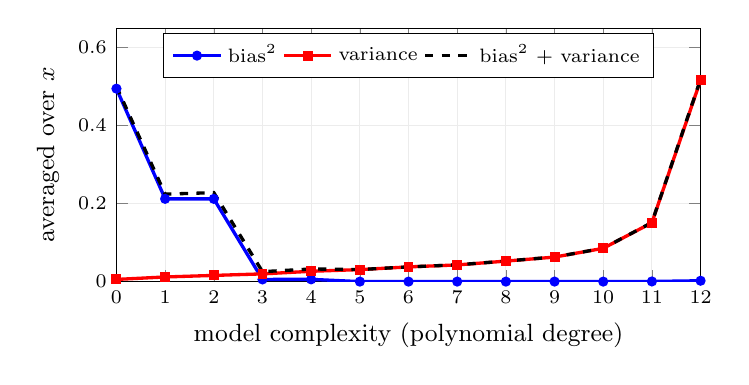
\begin{tikzpicture}
      \begin{axis}[width=9cm, height=4.8cm, xmin=0, xmax=12, ymin=0, ymax=0.65, xlabel={model complexity (polynomial degree)},
          ylabel={averaged over $x$}, tick label style={font=\scriptsize}, label style={font=\small}, xtick={0,...,12},
          legend style={font=\scriptsize, at={(0.5,0.98)}, anchor=north}, legend columns=3, grid=major, grid style={gray!15}]
        \addplot[blue, very thick, mark=*, mark size=1.2pt] coordinates {(0,0.4950) (1,0.2124) (2,0.2123) (3,0.0057) (4,0.0059) (5,0.0001) (6,0.0001) (7,0.0002) (8,0.0001) (9,0.0002) (10,0.0001) (11,0.0005) (12,0.0023)};
        \addlegendentry{bias$^2$}
        \addplot[red, very thick, mark=square*, mark size=1.2pt] coordinates {(0,0.0057) (1,0.0120) (2,0.0160) (3,0.0199) (4,0.0266) (5,0.0309) (6,0.0378) (7,0.0429) (8,0.0527) (9,0.0630) (10,0.0855) (11,0.1512) (12,0.5170)};
        \addlegendentry{variance}
        \addplot[black, very thick, dashed] coordinates {(0,0.5007) (1,0.2244) (2,0.2283) (3,0.0256) (4,0.0325) (5,0.0310) (6,0.0379) (7,0.0431) (8,0.0528) (9,0.0632) (10,0.0856) (11,0.1517) (12,0.5193)};
        \addlegendentry{bias$^2$ + variance}
      \end{axis}
    \end{tikzpicture}
    \caption{Bias--variance trade-off for polynomial regression. Many training sets $\mathcal D$ are drawn, each with $n=15$ noisy samples $f^*(x_j)+\varepsilon_j$ of $f^*(x)=\sin(2\pi x)$ at fixed positions $x_j$ (noise standard deviation $0.3$), and a polynomial $g(x;\mathcal D)$ is fitted by least squares to each. Top: $20$ fits (light red), their mean $E_{\mathcal D}\{g(x;\mathcal D)\}$ (dark red) and $f^*$ (dashed). A straight line is too rigid: all fits agree, but their mean misses $f^*$ (high bias, low variance). A degree-12 polynomial follows $f^*$ on average but varies strongly with the training set (low bias, high variance). Bottom: bias$^2$ and variance, averaged over $x$ and estimated from $400$ training sets per degree. The mean-square deviation from $f^*$ is smallest at an intermediate complexity.}
    \label{fig:bias_variance}
  \end{figure}

 \textbf {Bias-Variance Trade-Off:}
  \begin{itemize}
    \item Methods with \textbf{high flexibility} to adapt to the training data
      \begin{itemize}
        \item generally have low bias
        \item but yield high variance.            
      \end{itemize}
    \item Methods with \textbf{few parameters} and less degrees of freedom 
      \begin{itemize}
        \item tend to have a high bias, as they may not fit the data well. 
        \item However, this does not change a lot between different data sets, so these methods generally have low variance.            
      \end{itemize}
    \item Unfortunately, we can virtually never get both zero bias and zero variance!       
    \item We need to have as \textbf{much prior information} about the problem as possible to reduce both values.
  \end{itemize}
  
\subsubsection {Bias and Variance for Classification}

  Assuming a \textbf {two-class classification problem}:
  \begin{itemize}
    \item In a two-class problem, the target function changes to:
      \begin{displaymath}
        f^*(\vect x) = p(y = +1 \mid \vect x) = 1 - p(y = -1 \mid \vect x)
      \end{displaymath}
                 
    \item We cannot compare $g(\vect x ; {\mathcal{D}})$ and $f^*(\vect x)$ based on the mean-square error as in regression.
    \item For simplicity, let us assume \textbf{identical priors}: $p(y=+1)=p(y=-1)=\frac{1}{2}$.
      \begin{itemize}
        \item The Bayes-optimal prediction is $y^*(\vect x)=+1$ if $f^*(\vect x)\ge 0.5$ and $-1$ otherwise.
        \item The Bayes decision boundary is the set of points for which $f^*(\vect{x}) = 0.5$.
      \end{itemize}
  \end{itemize}
 \textbf{Boundary error}
    \begin{itemize}
    \item $p(g(\vect{x}; \mathcal{D}))$ is the density of obtaining a particular estimate of the discriminant given $\mathcal{D}$ (fixed $\vect x$, randomness comes from $\mathcal D$).
    \item Because of random variations in the training set, the boundary error depends upon this density.
  \end{itemize}

  \begin{displaymath}
    p\big(\hat y(\vect x;\mathcal D) \ne y^*(\vect x)\big) =
     \left\{
       \begin{array}{l l}
         \displaystyle{ \int_{0.5}^\infty p(g(\vect{x}; \mathcal{D})) \, \mathsf{d}g } & \mbox{if~} f^*(\vect{x}) < 0.5 \\
         \displaystyle{ \int_{-\infty}^{0.5} p(g(\vect{x}; \mathcal{D})) \, \mathsf{d}g } & \mbox{if~} f^*(\vect{x}) \ge 0.5
       \end{array}
     \right.
  \end{displaymath}

  \begin{itemize}
    \item Convenient assumption that \textbf{$p(g(\vect{x}; \mathcal{D}))$ is Gaussian}:
      \begin{eqnarray*}
        \lefteqn{p\big(\hat y(\vect x;\mathcal D) \ne y^*(\vect x)\big) =} \\
        & & \Phi \Bigg[ 
              \underbrace{\sign\left(f^*(\vect x) - \frac{1}{2}\right) \cdot \left(E_{\mathcal{D}} \{ g(\vect x ; {\mathcal{D}}) \} - \frac{1}{2}\right) }_{\mbox{\small \textbf{boundary bias}}}
              \cdot \underbrace{\mathsf{Var}_{\mathcal D}\!\Big[g(\vect x ; {\mathcal{D}})\Big]^{-1/2}}_{\mbox{\small \textbf{variance}}}
            \Bigg]
      \end{eqnarray*}
      where $\Phi$ is the \textbf{upper tail} of the standard normal:
      \begin{displaymath}
        \Phi(t) = \frac{1}{\sqrt{2\pi}} \int_t^\infty e^{-\frac{1}{2} u^2} \, \mathsf{d}u
      \end{displaymath}
    \item $p\big(\hat y(\vect x;\mathcal D) \ne y^*(\vect x)\big)$ represents the probability of incorrect estimation of the Bayes decision at $\vect x$.
  \end{itemize}
 
 \textbf{Conclusions:}

  \begin{itemize}
    \item In \textbf{regression} the bias-variance relation is additive in (bias)$^2$ and variance.     
    \item For \textbf {classification} the relation is multiplicative and nonlinear.        
    \item In classification the sign of the boundary bias affects the role of the variance in the error.            
    \item Therefore, low variance is generally important for accurate classification.
  \end{itemize}
         

 \textbf{Heuristic:} in classification, reducing the variance is often more effective than reducing the bias. This is not a theorem: the effect of bias and variance on the error depends on where the average boundary lies relative to the Bayes boundary, and neither term dominates universally.
  
  \def\covA{\mat{\Sigma}_i = \left(\begin{matrix} \sigma^2_{i1} & \sigma_{i12} \\ \sigma_{i12} & \sigma^2_{i2} \end{matrix}\right)}
  \def\covB{\mat{\Sigma}_i = \left(\begin{matrix} \sigma^2_{i1} & 0            \\ 0            & \sigma^2_{i2} \end{matrix}\right)}
  \def\covC{\mat{\Sigma}_i = \left(\begin{matrix} 1             & 0            \\ 0            & 1             \end{matrix}\right)}

\subsection{Estimating Bias and Variance}
Resampling for Estimating Statistics

 \textbf  {Problem:}
    \begin{itemize}
    \item Determine the bias and variance for some learning algorithm applied to a new problem with unknown distributions.
  \end{itemize}
   From what we have seen so far, bias and variance change with varying samples.
         

 \textbf {Resampling techniques} can be used to yield more informative estimates of a general statistics.\\
 \textbf  {Formally:}
 \begin{itemize}
    \item Suppose we want to estimate a parameter $\theta$ that depends on a random sample set $X = (x_1, \ldots, x_n)$.
    \item Assume we have an estimator $\phi_n(X)$ of $\theta$ but do not know its distribution.
   \item Resampling methods try to estimate the bias and variance of $\phi_n(X)$ using subsamples from $X$.
  \end{itemize}
  
\subsubsection{Jackknife}
  
  Let $\PS_i(X)$ be the $i$-th pseudovalue of $\phi_n(X)$:
  \begin{eqnarray*}
    \PS_i(X) 
      &=& n \phi_n(X) - (n-1) \phi_{n-1}(X_{(i)}) \\
      &=& \phi_n(X) - \underbrace{(n-1)( \phi_{n-1}(X_{(i)}) - \phi_n(X))}_{\mathsf{bias}_{\text{jack},i}}
  \end{eqnarray*}
  where $X_{(i)} = (x_1, \ldots, x_{i-1}, x_{i+1}, \ldots, x_n)$ is the set without the $i$-th element.\\
 \textbf {Notes:}
  \begin{itemize}
    \item $\PS_i(X)$ can be interpreted as a bias-corrected version of $\phi_n(X)$:        
    \item The bias trend is assumed to be in the estimators from $\phi_{n-1}(X_{(i)})$ to $\phi_n(X)$.
  \end{itemize}
 \textbf {Jackknife Principle:}
  \begin{itemize}
    \item The pseudovalues $\PS_i(X)$ are \emph{treated as if} they were independent random variables with mean $\theta$. (They are computed from overlapping leave-one-out sets and are actually dependent; the approximation works for sufficiently smooth statistics.)
    \item The jackknife estimate $\mu_{\PS}$ is approximately normal with variance $\sigma^2_{\PS}/n$.
    \item The estimators for the mean $\mu_{\PS}$ and variance $\sigma_{\PS}^2$ of the pseudovalues are the sample estimates:
      \begin{eqnarray*}
        \mu_{\PS}      &=& \frac{1}{n} \sum_{i=1}^n \PS_i(X) \\
        \sigma_{\PS}^2 &=& \frac{1}{n-1} \sum_{i=1}^n (\PS_i(X) - \mu_{\PS})^2
      \end{eqnarray*}
  \end{itemize}
 
  \begin{example}
    \small
    Estimator for the sample mean: $\phi_n(X) = \frac{1}{n} \sum_{i=1}^n x_i = \overline{X}$     Pseudovalues of $\phi_n(X)$:
    \begin{displaymath}
      \PS_i(X) = n\overline{X} - (n-1) \overline{X_{(i)}} = x_i
    \end{displaymath}
    Jackknife estimates:
    \begin{eqnarray*}
      \mu_{\PS}      &=& \frac{1}{n} \sum_{i=1}^n \PS_i(X) = \overline{X} \\
      \sigma_{\PS}^2 &=& \frac{1}{n-1} \sum_{i=1}^n (x_i - \overline{X})^2
    \end{eqnarray*}
    Estimator for sample variance: $\phi_n(X) = \frac{1}{n} \sum_{i=1}^n (x_i - \overline{X})^2$  
    Pseudovalues of $\phi_n(X)$:
    \begin{displaymath}
      \PS_i(X) = \frac{n}{n-1} (x_i - \overline{X})^2
    \end{displaymath}
    Which implies that:
    \begin{displaymath}
      \mu_{\PS} = \frac{1}{n} \sum_{i=1}^n \PS_i(X) = \frac{1}{n-1} \sum_{i=1}^n (x_i - \overline{X})^2
    \end{displaymath}
Interestingly:\\
    \begin{itemize}
      \item[ $\bullet$] $E\{\phi_n(X)\} = \frac{n-1}{n}\sigma^2$ whereas $E\{ \mu_{\PS} \} = \sigma^2$
      \item[ $\bullet$] $\mu_{\PS}$ is a bias-corrected version of $\phi_n(X)$
    \end{itemize}
  \end{example}
         
\subsubsection{Bootstrap}
  \begin{itemize}
    \item A \textit{bootstrap} data set is created by randomly selecting $n$ points from the sample set with replacement.            
    \item In \textit{bootstrap estimation} this selection process is independently repeated $B$ times.            
    \item The $B$ bootstrap data sets are treated as independent sets.
  \end{itemize}

  With $\hat\theta^{(b)}=\phi_n(X^{(b)})$ the estimate on the $b$-th bootstrap set $X^{(b)}$, $b=1,\dots,B$, the bootstrap estimate of the statistic $\theta$ and its variance are:
  \begin{eqnarray*}
    \mu_{\mathsf{BS}}      &=& \frac{1}{B} \sum_{b=1}^B \hat{\theta}^{(b)} \\
    \sigma^2_{\mathsf{BS}} &=& \frac{1}{B-1} \sum_{b=1}^B \left( \hat{\theta}^{(b)} - \mu_{\mathsf{BS}} \right)^2
  \end{eqnarray*}
  The bias is the difference between the bootstrap estimate and the estimator $\phi_n(X)$:
  \begin{displaymath}
    \mathsf{bias}_{\mathsf{BS}} = \mu_{\mathsf{BS}} - \phi_n(X)
  \end{displaymath}
 
 \textbf{Properties of the bootstrap estimate:}
  \begin{itemize}
    \item Bootstrap sets are drawn from the empirical distribution of the data (with replacement), so the class proportions are preserved in expectation.
    \item The larger the number $B$, the more the bootstrap estimate tends towards the ideal bootstrap estimate ($B\to\infty$).
    \item In contrast, the jackknife estimator requires exactly $n$ repetitions: 
      \begin{itemize}
        \item less than $n$ repetitions yield poorer estimates
        \item more than $n$ repetitions merely duplicate information already provided
      \end{itemize}
  \end{itemize}

\subsection{Estimating and Comparing Classifiers}

  Two reasons why we want to know the generalization rate of a classifier on a given problem:

  \begin{enumerate}
    \item to see if the classifier performs well enough to be useful
    \item to compare its performance with a competing design
  \end{enumerate}
\subsubsection{Cross-Validation}
  
  \begin{itemize}
    \item In \textbf{cross-validation}, the training samples are split into disjoint parts.
    \item An \textbf{$m$-fold cross-validation} splits the data into $m$ disjoint sets of size $n/m$ (here $m$ is the number of folds):
      \begin{itemize}
        \item 1 set is held out.
        \item The other $m-1$ sets are used for training.
        \item Each set is used once as held-out set.
      \end{itemize}
    \item The CV estimate is the average error over the $m$ held-out folds (weighted by fold size if folds differ in size).
    \item Note: if the held-out fold is used to stop training or to select parameters, it acts as a \textbf{validation} set and the best CV score is optimistic; the final error should be reported on separate \textbf{test} data (or with nested cross-validation).
    \item All data-dependent preprocessing (standardization, PCA, feature selection, \dots) must be fitted on the training folds only, not on the full data set.
    \item In the \textbf{extreme case of $m=n$}, we obtain a jackknife estimate of the classification accuracy.
  \end{itemize}
  The procedure is sketched in Fig.~\ref{fig:crossvalidation}.

  \begin{figure}[htbp]
    \centering
    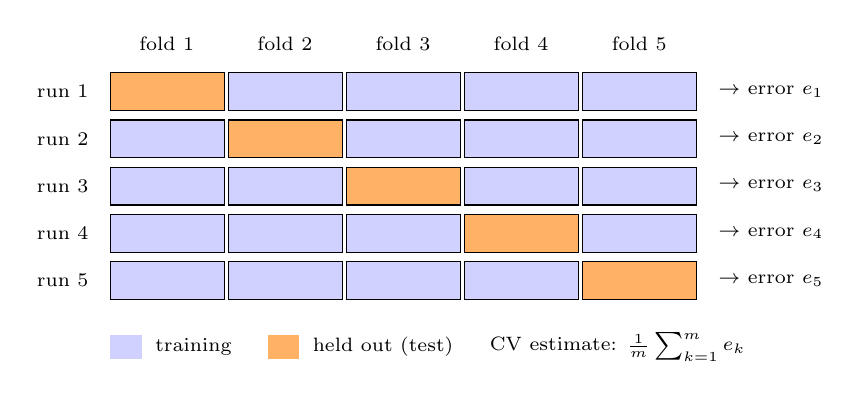
\begin{tikzpicture}[font=\small]
      \foreach \r in {1,...,5} {
        \foreach \c in {1,...,5} {
          \ifnum\r=\c \def\col{orange!60}\else\def\col{blue!18}\fi
          \fill[\col] (1.5*\c-1.5, -0.6*\r) rectangle (1.5*\c-0.05, -0.6*\r+0.48);
          \draw (1.5*\c-1.5, -0.6*\r) rectangle (1.5*\c-0.05, -0.6*\r+0.48);
        }
        \node[anchor=east, font=\scriptsize] at (-0.15, -0.6*\r+0.24) {run \r};
        \node[anchor=west, font=\scriptsize] at (7.6, -0.6*\r+0.24) {$\to$ error $e_{\r}$};
      }
      \foreach \c in {1,...,5} {\node[font=\scriptsize] at (1.5*\c-0.78, 0.25) {fold \c};}
      \fill[blue!18] (0,-3.75) rectangle (0.4,-3.45); \node[anchor=west, font=\scriptsize] at (0.45,-3.6) {training};
      \fill[orange!60] (2.0,-3.75) rectangle (2.4,-3.45); \node[anchor=west, font=\scriptsize] at (2.45,-3.6) {held out (test)};
      \node[anchor=west, font=\scriptsize] at (4.7,-3.6) {CV estimate: $\frac{1}{m}\sum_{k=1}^{m}e_k$};
    \end{tikzpicture}
    \caption{$m$-fold cross-validation with $m=5$. The data are split into $m$ disjoint folds; in run $k$, fold $k$ is held out and the classifier is trained on the other $m-1$ folds. Each sample is used exactly once for testing, and the CV estimate is the average of the $m$ held-out errors. For $m=n$ this becomes the leave-one-out (jackknife) estimate.}
    \label{fig:crossvalidation}
  \end{figure}

  For early stopping, the classifier is trained until a minimum error on a validation split (taken from the training part) is reached (good generalization vs.\ overfitting); the held-out evaluation fold must not be used for this.
   
\subsection{Lessons Learned}

  \begin{itemize}
    \item There is no such thing as a free lunch!              
    \item Bias-variance trade-off              
    \item Jackknife              
    \item Bootstrap              
    \item Cross-Validation
  \end{itemize}


\subsection{Comprehensive Questions}
 
  \begin{itemize}
    \item What is the meaning of the terms bias and variance?         
    \item What is the difference in bias-variance trade-off between regression and classification?         
    \item How do you estimate the bias and variance of a method?         
    \item What is cross-validation and how can it be used to train a classifier?
  \end{itemize}
          

\def\err{{\mathop{\overline{\mathsf{err}}}}}

\section{AdaBoost}\autocite{hastie2009,freund1997,matas,viola2001,viola2004}

\textbf{Notation in this Chapter}\\
{\small
\begin{itemize}
  \item $\mathcal D=\{(\vect x_i,y_i)\}_{i=1}^N$: training set of size $N$.
  \item $i$: sample index.
  \item $m=1,\dots,M$: boosting iteration.
  \item $y_i\in\{-1,+1\}$: true labels.
  \item $G_m(\vect x)\in\{-1,+1\}$: weak classifier in iteration $m$.
  \item $f_M(\vect x)=\sum_{m=1}^M \beta_m G_m(\vect x)$: additive model, $f_0\equiv0$; the algorithm box uses $\alpha_m=2\beta_m$, which gives the same sign.
  \item Final prediction: $\hat y = G(\vect x)=\sign(f_M(\vect x))$.
  \item $w_i^{(m)}$: weight of sample $i$ in boosting iteration $m$.
  \item $\mathbb I(\cdot)$: indicator function ($I(u,v)$ is reserved for the image intensity).
\end{itemize}
}

\subsection{Boosting methods}

  \begin{itemize}
    \item Boosting is one of the most powerful learning techniques introduced in the last twenty years.
    \item Combines output of many \textbf {\textit{weak} classifiers} to produce a powerful committee.
    \item The most popular boosting algorithm is called \textbf {\textit{AdaBoost}} \\
      (Freund and Schapire, 1997).
  \end{itemize}
\textbf{Definition:} A \textbf {weak classifier} is one whose error rate is only slightly better than random guessing.

 \subsubsection{Idea of boosting:}

  \begin{itemize}
    \item Sequentially apply the \emph{weak} classifier to repeatedly modified versions of the data.
    \item This produces a sequence of classifiers.
    \item Weighted majority vote yields the final prediction.
    \item Consider a two-class problem with $y \in \{ -1, +1\}$.          %           
    \item Given a set of observations $\mathcal{D} = \{(\vect{x}_i, y_i); \quad i=1,\ldots,N\}$ and a classifier $G(\vect x)$, the \textbf  {error rate} on the training sample is:
      \begin{displaymath}
        \err = \frac{1}{N} \sum_{i=1}^N \mathbb I(y_i \neq G(\vect{x}_i))
      \end{displaymath}
      where $\mathbb I$ is the \textbf  {indicator function}.
    \item Sequentially applied weak classifiers produce a sequence $G_m(\vect x)$ with $m=1,2,\ldots,M$ %           
    \item The \textbf{combined prediction} is then:
      \begin{displaymath}
        \hat y = G(\vect x) = \sign \left( \sum_{m=1}^M \alpha_m G_m(\vect x) \right)
      \end{displaymath}
      %           
    \item The weighting factors $\alpha_1, \ldots, \alpha_M$ are computed by the boosting algorithm. %           
    \item Each $\alpha_m$ weights the output of the corresponding classifier $G_m(\vect x)$.
  \end{itemize}

 \subsubsection{Schematic of boosting procedure:}

 \textbf{Modifications on the data:}

  \begin{itemize}
    \item Each boosting step consists of applying weights $w_1, w_2, \ldots, w_N$ to the training samples.
    \item Initially, the weights are set to $w_i = 1/N$.
    \item Thus the first classifier in the sequence is trained the usual way. %           
    \item For $m \geq 2$ the weights are individually modified. %           
    \item The classifiers $G_m$, with $m \geq 2$ are trained on differently-weighted samples.
  \end{itemize}
 
 \textbf {Weighting scheme:}
  \begin{itemize}
    \item At step $m$ the misclassified observations from $G_{m-1}$ have increased weights.
    \item The weights for correctly classified samples from $G_{m-1}$ have decreased weights.
  \end{itemize}
         

 \textbf {Effects of the weighting scheme:}
  \begin{itemize}
    \item Observations that are difficult to classify correctly get ever-increasing influence.
    \item Each successive classifier is forced to concentrate more on those observations that were misclassified by the previous one.
  \end{itemize}
 
\subsection{AdaBoost}

 \textbf {AdaBoost algorithm:}
%
  \begin{centernss}
    \small
      \begin{struktogramm}(100,62)\\
        \assign{Initialize weights: $w_i \gets 1/N ~,~ i=1, \ldots, N$}
        \assign{$m \gets 1$}
        \until{$m > M$}\\
          \assign{{Fit classifier $G_m(\vect x)$ to training data using weights $w_1,\dots,w_N$}}\\
          \assign{{Compute classification error:}\\
            $ \mathsf{err}_m = \frac{\sum_{i=1}^N w_i \mathbb I(y_i \neq G_m(\vect x_i))}{\sum_{i=1}^N w_i}$
          }\\
          \assign{{Compute classifier weights:}\\
            $ \alpha_m = \log \left( \frac{1- \mathsf{err}_m}{\mathsf{err}_m} \right) $
          }\\
          \assign{{Compute new sample weights:}\\
            $ w_i \leftarrow w_i \exp \left[ \alpha_m \mathbb I(y_i \neq G_m(\vect x_i)) \right] ~,~ i = 1, \ldots, N $
          }
          \assign{$m \gets m + 1$}\\
        \untilend
        \assign{\textbf{Output:} $\hat y = G(\vect x) = \sign \left( \sum_{m=1}^M \alpha_m G_m(\vect x) \right) $}
      \end{struktogramm}
    
  \end{centernss}
 \textbf {Notes:}
  \begin{itemize}
    \item This version of AdaBoost is called \textbf {discrete}, because each $G_m(\vect x)$ returns a discrete class label. %           
    \item AdaBoost can be modified to return also a real-valued prediction in the interval $[-1,+1]$.  % 
    \item Instead of taking just any classifier for $G_m(\vect x)$, that classifier may be used that results in the smallest error at step $m$.
  \end{itemize}

  AdaBoost dramatically increases the performance of even a very weak classifier.
 
\subsection{Exponential Loss}

  \begin{itemize}
    \item Boosting fits an \textbf{additive model} in a \textbf{set of elementary basis functions}:
      \begin{displaymath}
        f(\vect x)=\sum_{m=1}^{M} \beta_m\, b(\vect x;\vect\gamma_m),
      \end{displaymath}
      where $\beta_m$ are expansion coefficients and $b(\vect x;\vect \gamma_m)$ is a basis function with parameters $\vect \gamma_m$.
    \item Additive expansions are very popular in learning techniques:
      \begin{itemize}
        \item single-hidden-layer neural networks (perceptron)
        \item wavelets
        \item classification trees
        \item etc.
      \end{itemize}
  \end{itemize}
  
  \begin{itemize}
    \item Expansion models are typically fit by \textbf{minimizing a loss function $L$} averaged over the training data:
      \begin{equation} 
        \label{eq:loss}
        \min_{\{ \beta_m, \vect \gamma_m \}_1^M } ~ 
        \left\{
          \sum_{i=1}^N L \big( y_i, f_M(\vect{x}_i) \big) =
          \sum_{i=1}^N L \left( y_i, \sum_{m=1}^M \beta_m \, b(\vect{x}_i ; \vect \gamma_m) \right)
        \right\}
      \end{equation}
                           
    \item\textbf  {Forward stagewise modeling} approximates the solution to \eqref{eq:loss}:
      \begin{itemize}
        \item New basis functions are sequentially added.          
        \item Parameters and coefficients of already added functions are not changed.
        \item At each iteration, the subproblem of fitting just a single basis function is solved.
      \end{itemize}
  \end{itemize}
          
  \begin{itemize}
    \item The \textbf {$m$-th subproblem} may be rewritten as:              
      \begin{center}
            $
              \displaystyle
              (\beta_m, \vect \gamma_m) = \argmin_{\beta, \vect \gamma} ~\sum_{i=1}^N L\big(y_i, f_{m-1}(\vect{x}_i) + \beta \, b(\vect{x}_i ; \vect{\gamma})\big)
            $
      \end{center}
    \item AdaBoost is equivalent to a forward stagewise additive modeling using an \textbf {exponential loss function}:
      \begin{displaymath}
        L(y, f(\vect x)) = \exp (-y \, f(\vect x))
      \end{displaymath}
  \end{itemize}
  \textbf {Proof:}

  \begin{itemize}
    \item For AdaBoost, the basis functions are the classifiers $G_m(\vect x) \in \{-1,+1\}$.
    \item Using the \textbf{exponential loss function}, one must solve at each step:
      \begin{eqnarray*}
        (\beta_m, G_m) = \argmin_{\beta, G} ~\sum_{i=1}^N \exp \left[ -y_i \big(f_{m-1}(\vect{x}_i) + \beta G(\vect{x}_i)\big) \right]
      \end{eqnarray*}
    \item Using the weight $w_i^{(m)} = \exp(-y_i \, f_{m-1}(\vect{x}_i))$ (so $w_i^{(1)}=1$ since $f_0\equiv0$) this can be rewritten as:
      \begin{eqnarray*}
        (\beta_m, G_m) = \argmin_{\beta, G} ~\sum_{i=1}^N w_i^{(m)} \exp (-\beta y_i G(\vect{x}_i))
      \end{eqnarray*}
  \end{itemize}

 \textbf {Observations:}
  \begin{itemize}
    \item Since $w_i^{(m)}$ is independent of $\beta$ and $G(\vect x)$, it can be seen as a weight applied to each observation.
    \item However, this weight depends on $f_{m-1}$, so the weights change with each iteration $m$.
  \end{itemize}

  \begin{eqnarray*}
    (\beta_m, G_m) 
      &=& \argmin_{\beta, G} ~\sum_{i=1}^N w_i^{(m)} \exp (-\beta y_i G(\vect{x}_i)) \\ 
      &=& \argmin_{\beta, G} ~ e^{-\beta} \sum_{y_i = G(\vect{x}_i)} w_i^{(m)} + e^{\beta} \sum_{y_i \neq G(\vect{x}_i)} w_i^{(m)} \\ 
      &=& \argmin_{\beta, G} ~ \left( e^{\beta} - e^{-\beta} \right) \sum_{i=1}^N w_i^{(m)} \mathbb I(y_i \neq G(\vect{x}_i)) + e^{-\beta} \sum_{i=1}^N w_i^{(m)}
  \end{eqnarray*}

  \begin{itemize}
    \item The weight scaling is irrelevant for selecting $G_m$ (positive scaling does not change the argmin).
    \item Plugging the optimal $G_m(\vect x)$ into the objective function and solving for $\beta_m$: with the \textbf{minimized weighted error rate}
      \begin{displaymath}
        \mathsf{err}_m = \frac{\sum_{i=1}^N w_i^{(m)} \mathbb I(y_i \neq G_m(\vect{x}_i))}{\sum_{i=1}^N w_i^{(m)}}
      \end{displaymath}
      the objective (divided by $\sum_i w_i^{(m)}$) is $(e^{\beta}-e^{-\beta})\,\mathsf{err}_m+e^{-\beta}$. Setting its derivative to zero gives $(e^{\beta}+e^{-\beta})\,\mathsf{err}_m=e^{-\beta}$, i.\,e.\ $e^{2\beta}=\frac{1-\mathsf{err}_m}{\mathsf{err}_m}$:
      \begin{displaymath}
        \beta_m=\frac12\log\frac{1-\mathsf{err}_m}{\mathsf{err}_m}.
      \end{displaymath}
     \item From the update formula of the approximation:
      \begin{eqnarray*}
        f_m(\vect x) = f_{m-1}(\vect x) + \beta_m \, G_m(\vect x)
      \end{eqnarray*}
      we can calculate the \textbf{weights for the next iteration}:
      \begin{align*}
        w_i^{(m+1)}
          &= w_i^{(m)} \, e^{-\beta_m y_i G_m(\vect{x}_i)} \\
          &\qquad \text{(using: $-y_i G_m(\vect{x}_i) = 2 \mathbb I(y_i \neq G_m(\vect{x}_i)) - 1$)} \\
          &= w_i^{(m)} \, e^{\alpha_m \mathbb I(y_i \neq G_m(\vect{x}_i))} \, e^{-\beta_m}
      \end{align*}
      with $\alpha_m = 2 \beta_m$ and thus $\hat y = \sign(f_M(\vect x))$.
  \end{itemize}
 

 \textbf {Compare result to initial AdaBoost algorithm:}

  \begin{itemize}
    \item\textbf {Exponential loss:}
      \begin{eqnarray*}
        \beta_m     &=& \frac{1}{2} \log \frac{1 - \mathsf{err}_m}{\mathsf{err}_m} \\
        \alpha_m    &=& 2 \beta_m \\
        w_i^{(m+1)} &=& w_i^{(m)} ~ e^{\alpha_m \mathbb I(y_i \neq G_m(\vect{x}_i))} ~ e^{-\beta_m}
      \end{eqnarray*}
             
    \item\textbf {AdaBoost:}
      \begin{eqnarray*}
        \alpha_m &=&          \log \frac{1- \mathsf{err}_m}{\mathsf{err}_m} \\
        w_i      &\leftarrow& w_i \, e^{\alpha_m \mathbb I(y_i \neq G_m(\vect{x}_i))}
      \end{eqnarray*}
  \end{itemize}
          


 
 \textbf {Discussion:}

  \begin{itemize}
    \item The equivalence of AdaBoost to forward stagewise additive modeling was discovered five years after its invention. %           
    \item The AdaBoost criterion yields a monotone decreasing function of the \textbf        {margin}: $y\,f(\vect x)$.          %           
    \item In $\{-1, +1\}$ classification, the margin plays a role similar to the \\
      residuals $y - f(\vect x)$ in regression:
      \begin{itemize}
        \item Observations with $y_i \, f(\vect{x}_i) > 0$ are classified correctly
        \item Observations with $y_i \, f(\vect{x}_i) < 0$ are misclassified 
        \item The decision boundary is at $f(\vect x) = 0$
     \end{itemize}
   \item The goal of the classification algorithm is to produce positive margins as frequently as possible. % 
    \item Thus, any loss criterion should penalize negative margins more heavily than positive ones! % 
    \item The exponential criterion concentrates much more influence on observations with large negative margins.
  \end{itemize}
 
  Due to the exponential loss, AdaBoost performance is known to degrade rapidly:
  \begin{itemize}
    \item in situations of noisy data
    \item when there are wrong class labels in the training data
  \end{itemize}
 
\subsection{Face Detection}

  Famous algorithm developed by \textbf {Viola and Jones} in 2001.
 \textbf{Contributions:}

  \begin{itemize}
    \item Integral images for feature computation.
    \item Usage of AdaBoost for boosting.
    \item Classifier cascade for fast rejection of non-face regions.
  \end{itemize}

  Various implementations available: for example look into \textit{OpenCV FaceDetector} sample code.
 
 \textbf{Features:}

  \begin{itemize}
    \item Features are adapted from Haar basis functions. %           
    \item They are calculated by subtracting the sum of the pixels in the white from the sum of the pixels in the gray rectangles:               %           
  \end{itemize}

 4 types of features used (Fig.~\ref{fig:vj_haar}):
  \begin{itemize}
    \item The exhaustive set of Haar-like rectangle features is very large (in the classic Viola--Jones setup this count refers to the $24\times 24$ detection window, not to the full image). %
    \item Rectangle features can be efficiently computed using an \\
    \textbf {Integral Image $II$}:
      \begin{displaymath}
        II(u,v) = \sum_{u' \leq u, v' \leq v} I(u', v')
      \end{displaymath}
      where $I(u',v')$ is the image intensity at pixel $(u',v')$ (pixel coordinates $(u,v)$, since $\vect x$ denotes the image sub-window).
  \end{itemize}

The sum of intensities over any rectangle needs only four look-ups in the integral image (three additions/subtractions); see Fig.~\ref{fig:vj_integral}.\\

  \begin{figure}[htbp]
    \centering
    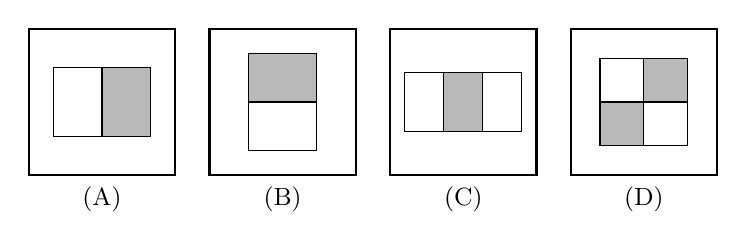
\begin{tikzpicture}[scale=0.62, font=\small]
      \tikzset{win/.style={draw, thick}, gr/.style={fill=gray!55, draw}, wh/.style={fill=white, draw}}
      % (A) two-rectangle, horizontal
      \begin{scope}
        \draw[win] (0,0) rectangle (3,3);
        \draw[wh] (0.5,0.8) rectangle (1.5,2.2); \draw[gr] (1.5,0.8) rectangle (2.5,2.2);
        \node at (1.5,-0.5) {(A)};
      \end{scope}
      % (B) two-rectangle, vertical
      \begin{scope}[xshift=3.7cm]
        \draw[win] (0,0) rectangle (3,3);
        \draw[gr] (0.8,1.5) rectangle (2.2,2.5); \draw[wh] (0.8,0.5) rectangle (2.2,1.5);
        \node at (1.5,-0.5) {(B)};
      \end{scope}
      % (C) three-rectangle
      \begin{scope}[xshift=7.4cm]
        \draw[win] (0,0) rectangle (3,3);
        \draw[wh] (0.3,0.9) rectangle (1.1,2.1); \draw[gr] (1.1,0.9) rectangle (1.9,2.1); \draw[wh] (1.9,0.9) rectangle (2.7,2.1);
        \node at (1.5,-0.5) {(C)};
      \end{scope}
      % (D) four-rectangle
      \begin{scope}[xshift=11.1cm]
        \draw[win] (0,0) rectangle (3,3);
        \draw[wh] (0.6,1.5) rectangle (1.5,2.4); \draw[gr] (1.5,1.5) rectangle (2.4,2.4);
        \draw[gr] (0.6,0.6) rectangle (1.5,1.5); \draw[wh] (1.5,0.6) rectangle (2.4,1.5);
        \node at (1.5,-0.5) {(D)};
      \end{scope}
    \end{tikzpicture}
    \caption{The four types of Haar-like rectangle features inside the detection window: two-rectangle features (A, B), a three-rectangle feature (C) and a four-rectangle feature (D). The feature value $\phi_j(\vect x)$ is the sum of the pixel intensities in the gray rectangles minus the sum in the white rectangles. Position, size and type of the rectangles are varied over the whole $24\times24$ window, which gives the very large set of candidate features from which AdaBoost selects.}
    \label{fig:vj_haar}
  \end{figure}

  \begin{figure}[htbp]
    \centering
    \begin{tikzpicture}[scale=0.8, font=\small, >={Stealth}]
      % left: definition of II(u,v)
      \begin{scope}
        \draw[thick] (0,0) rectangle (5,4);
        \fill[blue!20] (0,4) rectangle (3,1.5);
        \draw[blue, thick] (0,4) rectangle (3,1.5);
        \fill (3,1.5) circle (2.5pt) node[below right] {$(u,v)$};
        \node[blue!60!black, align=center] at (1.5,2.75) {$II(u,v)$};
        \draw[->] (-0.3,4.3) -- (1.2,4.3) node[right] {$u$};
        \draw[->] (-0.3,4.3) -- (-0.3,2.9) node[below] {$v$};
        \node[align=center, font=\footnotesize, text width=4.2cm] at (2.5,-0.7) {$II(u,v)$: sum of all pixels above and to the left of $(u,v)$};
      \end{scope}
      % right: rectangle sum with four look-ups
      \begin{scope}[xshift=6.6cm]
        \draw[thick] (0,0) rectangle (5,4);
        \draw (0,4) rectangle (2,2.5); \node at (1,3.25) {$A$};
        \draw (2,4) rectangle (4,2.5); \node at (3,3.25) {$B$};
        \draw (0,2.5) rectangle (2,0.8); \node at (1,1.65) {$C$};
        \fill[orange!35] (2,2.5) rectangle (4,0.8); \draw[thick] (2,2.5) rectangle (4,0.8); \node at (3,1.65) {$D$};
        \foreach \p/\n/\a in {(2,2.5)/1/above left, (4,2.5)/2/above right, (2,0.8)/3/below left, (4,0.8)/4/below right}
          {\fill \p circle (2.5pt) node[\a, font=\footnotesize] {\n};}
        \node[align=center, font=\footnotesize, text width=4.2cm] at (2.5,-0.7) {$\sum_D I = II(4)-II(2)$\\$-\,II(3)+II(1)$};
      \end{scope}
    \end{tikzpicture}
    \caption{Integral image. Left: $II(u,v)$ stores the sum of all intensities $I(u',v')$ with $u'\le u$, $v'\le v$; it is computed in one pass over the image. Right: with the corner values $II(1)=A$, $II(2)=A+B$, $II(3)=A+C$ and $II(4)=A+B+C+D$ (letters denoting region sums), the sum over any rectangle $D$ needs only four look-ups: $D=II(4)-II(2)-II(3)+II(1)$. A rectangle feature therefore costs a constant number of operations, independent of its size.}
    \label{fig:vj_integral}
  \end{figure}
 \textbf {Boosting:}\\

  \begin{itemize}
    \item The classification functions are restricted to each depend on a single feature only. %           
    \item This way, AdaBoost can be interpreted as an effective feature selecting algorithm:
      \begin{itemize}
        \item The single rectangle feature is selected which best separates the observations. %  
        \item For each feature, the weak learner determines the optimal threshold classification function.
      \end{itemize}
     \item A weak classifier $G_j(\vect x)$ consists of a \textbf{feature value $\phi_j(\vect x)$} ($j$: feature index), an \textbf {optimal threshold $\theta_j$}, and a \textbf{parity $s_j$} to indicate the direction of the inequality:
      \begin{displaymath}
        G_j(\vect x) = \begin{cases}
                        +1 \quad \mbox{if} ~s_j \phi_j(\vect x) < s_j \theta_j \\
                        -1 \quad \mbox{otherwise}
                      \end{cases}
      \end{displaymath}
      with $\vect x$ being a sub-window of an image. (Viola and Jones use $G_j\in\{0,1\}$ and decide ``face'' iff $\sum_m\alpha_m G_m\ge\frac12\sum_m\alpha_m$; with $\pm1$ outputs this is the sign rule above.)
    \item Very aggressive process to discard the vast majority of features.
 \item The best features selected by AdaBoost are shown in the slides.
  \end{itemize}
 \textbf {Classifier Cascade:}

  \begin{itemize}
    \item Despite the efficiency of the feature computation, the complexity of the problem is still huge. %           
    \item Evaluating the full AdaBoost sequence on all sub-windows of the image takes too much time.
    \item Idea of cascaded classifiers:
    \begin{itemize}
      \item Simpler classifiers used to reject the majority of sub-windows. %           
      \item Each stage is again created by AdaBoost. %           
      \item Stage 1 uses the two best features; it detects 100\,\% of the faces (true positive rate, TPR) with a false positive rate (FPR) of around 40\,\% (rates as defined in Chapter~1).
    \end{itemize}
  \end{itemize}

  \begin{itemize}
    \item The cascade has the overall shape of a degenerated decision tree (Fig.~\ref{fig:vj_cascade}):         
    \item A negative classification at any stage yields an immediate rejection of the sub-window.
    \item Structure of cascade reflects the (usually) overwhelming majority of negative sub-windows in an image. %           
    \item Goal is to reject as many negatives as possible at the earliest stage of the processing.
  \end{itemize}

  \begin{figure}[htbp]
    \centering
    \begin{tikzpicture}[font=\small, >={Stealth}, node distance=0.6cm and 0.75cm,
        st/.style={draw, thick, circle, minimum size=0.95cm, fill=gray!10, align=center, inner sep=1pt},
        io/.style={draw, rounded corners, align=center, inner sep=3pt}]
      \node[io] (in) {all\\sub-windows};
      \node[st, right=of in] (s1) {1};
      \node[st, right=of s1] (s2) {2};
      \node[st, right=of s2] (s3) {3};
      \node[right=0.5cm of s3] (dots) {$\cdots$};
      \node[io, right=0.5cm of dots, fill=green!10] (out) {face};
      \node[io, below=1.1cm of s2, fill=red!8, minimum width=4.6cm] (rej) {reject sub-window};
      \draw[->, thick] (in) -- (s1);
      \draw[->, thick] (s1) -- node[above, font=\scriptsize] {T} (s2);
      \draw[->, thick] (s2) -- node[above, font=\scriptsize] {T} (s3);
      \draw[->, thick] (s3) -- node[above, font=\scriptsize] {T} (dots);
      \draw[->, thick] (dots) -- (out);
      \foreach \s in {s1,s2,s3} {\draw[->, thick, red!70!black] (\s) -- node[right, font=\scriptsize] {F} (\s |- rej.north);}
    \end{tikzpicture}
    \caption{Attentional cascade. Each stage is a boosted classifier tuned for a very high detection rate. A sub-window is passed on only if a stage accepts it (T); any rejection (F) discards it immediately. Since the vast majority of sub-windows contain no face, most of them are rejected by the first, very cheap stages (stage 1 uses only two features), and only the few face-like windows reach the expensive later stages. The overall rates are the products of the stage rates, e.\,g.\ with $10$ stages of TPR $0.99$ and FPR $0.3$: TPR $\approx0.99^{10}\approx0.90$, FPR $\approx0.3^{10}\approx6\cdot10^{-6}$.}
    \label{fig:vj_cascade}
  \end{figure}
  
 \textbf {Training of the cascade:}

  \begin{itemize}
    \item Subsequent classifiers are trained using only those examples which pass through all the previous stages. %           
    \item The next classifier faces a more difficult task than the previous one. 
    \item Trade-off between more features achieving higher detection rates and lower false positive rates while requiring more computation time.
  \end{itemize}
 \textbf {Final classifier:}
refer to slides for more details. 
  \begin{itemize}
    \setlength\itemsep{0.5cm}
    \item 32 layer cascade of increasingly strong boosted classifiers
    
    \begin{center}
      \begin{tabular}{r@{}l r c c}
        \multicolumn{2}{c}{\structure{Layer}} & 
       \textbf        {\# Features} & 
       \textbf        {TPR} &
       \textbf        {FPR}\\
        \hline
           &1  &   2~~~~~ & 100\,\% & 40\,\% \\
           &2  &   5~~~~~ & 100\,\% & 20\,\% \\
         3-&5  &  20~~~~~ & \\
         6-&7  &  50~~~~~ & \\
         8-&12 & 100~~~~~ & \\
        13-&32 & 200~~~~~ & \\ %           
      \end{tabular}
    \end{center}

    \item Number of stages and features adapted until false positive rate on validation was nearly zero while maintaining high correct rate.
  \end{itemize}

\subsection{Lessons Learned}

  \begin{itemize}
    \item Boosting of weak classifiers can yield a powerful combined classifier          
    \item AdaBoost algorithm              
    \item Weights of the classifiers and on the data are adjusted              
    \item AdaBoost minimizes an exponential loss function
    \item Viola \& Jones face detection algorithm
  \end{itemize}


          
